\chapter{一般学习问题的可学习性}
\label{chap:convex-learning-and-stability}

前两章讨论分类：学习算法输出一个分类器，零一损失只记录它是否预测正确。温度预测还要区分误差大小。若真实温度为20，两个模型分别预测18和10，零一损失把二者都记为错误，平方损失则分别给出4和100。聚类更进一步，它没有给定的正确标签，$K$均值的决策是一组中心，损失是观测到最近中心的平方距离。这些任务都依据训练样本选出一个完整决策，再以新观测上的平均损失评价它。本章研究：在这些不同任务中，怎样保证算法输出的期望风险接近比较决策空间中的最低水平？

第~\ref{sec:pac-general-form}节已经给出一般损失下的观测、决策、两种风险与PAC目标，第~\ref{sec:risk-comparison}节又建立了一条共同推理：只要同一事件上所有候选的总体—经验偏差都受控，再加上经验求解容差，就能得到超额风险上界；对重复训练取期望时，期望泛化差与平均经验优化误差给出平均超额风险的上界。前两章在零一损失下用VC维、图维等组合量取得那个共同偏差事件。换成一般损失后，这条路线有两处改变。第一，损失取连续值，$n$个观测上的损失向量不再只有有限多种，“数预测模式”的计数需要换成按数值精度衡量的容量。第二，一致收敛要求同一份样本估准所有决策的风险，其中包括算法根本不会选择的决策；一般损失允许出现这样的决策空间，使这一要求比学习本身更苛刻。

本章按“问题—工具—算法保证”展开。7.1节把预测函数类换成损失函数类，用伪维和胖打散维衡量实值损失的容量，并给出一个可学习却不满足一致收敛的例子，说明需要哪些新的分析。7.2节建立四类泛化分析工具：数据依赖的复杂度直接计算函数类在实际样本上追随随机噪声的能力；其余三类考察算法输出本身，样本压缩问输出能否由少数训练记录重构，信息方法衡量输出透露了多少关于样本的信息，并由同一个换测度不等式导出互信息界与PAC--Bayes界，算法稳定性比较替换或删除一条观测前后的两次输出。7.2节末再比较后三者各自控制的对象与相互联系。这些工具只提供风险比较所需的统计控制，不保证算法已经找到经验风险低的结果。7.3节再把它们用于模型选择、集成学习、正则化和梯度下降，说明具体程序怎样同时满足统计条件与经验拟合条件。

本章沿用第~\ref{sec:pac-general-form}节的记号：观测$z$属于观测空间$Z$，允许的分布组成分布族$\mathfrak P$，样本$S=(z_1,\ldots,z_n)$独立取自某个$\mathcal P\in\mathfrak P$；损失$\ell(w,z)$评价决策$w$在观测$z$上的表现；$R_{\mathcal P}(w)$与$\hat R_S(w)$分别是定义~\ref{def:general-population-risk}与定义~\ref{def:general-empirical-risk}中的期望风险与经验风险。算法可以使用独立于样本的内部随机数$U$，输出$A(S,U)$。除非另行说明，输出属于比较决策空间$\mathcal W$；上确界、算法与期望涉及的可测性按第~\ref{sec:measurability-convention}节的约定处理，每个定理只写出它额外需要的条件。
\section{一般损失问题与一致收敛}
\label{sec:real-valued-classes}
\label{sec:general-learning-problem}

前两章的充分路线是：限制候选空间的复杂程度，使同一份样本能同时估准所有候选的风险，再按经验风险选择。本节检查这条路线在一般损失下怎样推广，依次回答三个问题：一致收敛要控制哪个函数类；实值函数的复杂程度怎样按数值精度衡量；这种对整个类的控制对学习而言是否必要。

\subsection{从预测函数类到损失函数类}

风险是损失的平均，不是预测值的平均。因此，每个决策先对应一个从观测到损失值的函数，所有决策对应的函数组成\term{损失类}
\[
 \mathcal F_\ell=\{z\mapsto\ell(w,z):w\in\mathcal W\}.
\]
决策$w$的经验风险就是函数$\ell(w,\cdot)$在样本上的平均，期望风险是它在总体上的平均。要由经验风险推断期望风险，需要控制的是$\mathcal F_\ell$中函数的样本平均与总体平均之差。

同一组预测函数配上不同损失，得到的损失类可能在有界性和复杂度上都不同，所以不能直接把预测函数类的维度代入风险界。以一维线性预测$w(x)=ax$为例，令$|a|\leq1$、$|x|\leq1$。若标签$y\in[-1,1]$，平方损失$(ax-y)^2$取值于$[0,4]$，绝对损失$|ax-y|$取值于$[0,2]$，二者都有界；若允许$y$取任意实数，同一预测类的两种损失都失去有界性，后面依赖有界性的集中不等式便不能直接使用。复杂度也会改变：预测值$ax$关于$a$单调，而平方损失$(ax-y)^2$关于$a$先降后升，同一个$a$的变化在不同观测上可能使损失朝相反方向移动。可测性同样要按损失类核对：预测函数可测并配上可测损失时，单个损失函数可测；对整个类取上确界时，仍需按第~\ref{sec:measurability-convention}节的约定选取可数逼近子类。$K$均值的损失$\min_j\|x-c_j\|_2^2$说明，即使没有标签，也要从决策与损失共同确定的函数类出发分析。

确定损失类后，一致收敛的要求与第~\ref{sec:binary-uniform-convergence}节相同：同一份样本把损失类中每个函数的期望都估计准确。

% 保留旧位置锚点；在一般损失上使用一致收敛条件。
\phantomsection\label{def:general-uniform-convergence}
若对任意$\eta,\delta\in(0,1)$，存在不依赖分布的样本量$n_{\mathrm{uc}}(\eta,\delta)$，使每个$\mathcal P\in\mathfrak P$和每个$n\geq n_{\mathrm{uc}}(\eta,\delta)$都满足
\[
 \mathbb P_{S\sim\mathcal P^n}\!\left\{
 \sup_{w\in\mathcal W}|\hat R_S(w)-R_{\mathcal P}(w)|\leq\eta
 \right\}\geq1-\delta,
\]
就称损失类在允许族$\mathfrak P$上满足统一的一致收敛。样本量可以依赖决策空间、损失、精度和置信度，但对族内每个分布必须相同；只有当$\mathfrak P$包含观测空间上的全部相关分布时，才称为分布无关的一致收敛。本章各种稳定性条件也保留同一区分。

一致收敛事件正是第~\ref{sec:risk-comparison}节高概率比较所需的共同偏差事件。设在某份样本上
\[
 \sup_{w\in\mathcal W}|\hat R_S(w)-R_{\mathcal P}(w)|\leq\eta,\qquad
 \hat R_S(A(S))\leq\inf_{w\in\mathcal W}\hat R_S(w)+\alpha .
\]
定理~\ref{thm:approximate-erm-risk}的三步比较（输出的期望风险换成经验风险，经验近似最优，再把参照决策的经验风险换回期望风险）只用到这两个不等式和输出属于$\mathcal W$，不依赖损失取0或1，所以在同一事件上给出$R_{\mathcal P}(A(S))\leq\inf_wR_{\mathcal P}(w)+2\eta+\alpha$。一般损失新增的工作只在于核对：损失可积且所需上确界可测，偏差事件的概率由有界性或尾部条件支持。下面把这一推论写成学习保证。

\begin{theorem}[一致收敛推出一般学习保证]
\label{thm:general-uniform-pac}
设$(Z,\mathcal Z)$为可测观测空间，$(\mathcal W,\mathcal B_{\mathcal W})$为非空可测决策空间，$\mathfrak P$为$Z$上的一族概率分布，损失$\ell:\mathcal W\times Z\to\mathbb R$可测，且对每个$\mathcal P\in\mathfrak P$和$w\in\mathcal W$都有$\ell(w,\cdot)\in L^1(\mathcal P)$；假定所用上确界及相关事件可测。若损失类在$\mathfrak P$上满足统一的一致收敛，且确定性可测算法$A_n:Z^n\to\mathcal W$存在不依赖$\mathcal P$的$\alpha_n\to0$，使每份$S\in Z^n$都满足
\[
 \hat R_S(A_n(S))\leq\inf_{w\in\mathcal W}\hat R_S(w)+\alpha_n,
\]
则该算法相对于$\mathfrak P$统一地PAC学习此问题；$\mathfrak P$包含全部相关分布时，这是分布无关的PAC学习。
\end{theorem}
\begin{proof}
给定$\varepsilon,\delta\in(0,1)$，取$\eta=\varepsilon/4$，再取$n_1$使$n\geq n_1$时$\alpha_n\leq\varepsilon/2$。当$n\geq\max\{n_1,n_{\mathrm{uc}}(\varepsilon/4,\delta)\}$时，一致收敛事件的概率至少为$1-\delta$；在该事件上，前述比较给出超额风险至多$2\eta+\alpha_n\leq\varepsilon$。两个门槛都不依赖$\mathcal P$。
\end{proof}

这一定理只说明一致收敛加上足够小的经验求解容差就能保证学习，没有用到凸性，也没有说明怎样判断一致收敛是否成立。下一小节建立实值损失类的容量，再回到它是否必要的问题。
\subsection{伪维、胖打散维与数值精度}
\label{sec:comb-real-valued-threshold-margins}
\label{sec:comb-threshold-patterns}
\label{sec:comb-margin-patterns}

零一损失下，$n$个观测上的损失向量属于$\{0,1\}^n$，至多$2^n$种，VC维限制实际出现的种数，计数论证由此展开。换成平方损失后，即使只有一个观测，预测值连续变化也会给出连续多种损失值，精确计数失去意义。不过可以人为制造0/1模式：在每个输入处指定一个阈值，只记录函数值位于阈值上方还是下方。阈值对全部模式保持不变，实现不同模式的函数可以不同。

\begin{definition}[伪打散]
\label{def:pseudo-shattering}
设$\mathcal F\subseteq\mathbb R^{\mathcal X}$。有限集$C=\{x_1,\ldots,x_m\}$被$\mathcal F$\term{伪打散}（pseudo-shattering），是指存在$r_1,\ldots,r_m\in\mathbb R$，使任意$\bm b\in\{0,1\}^m$都对应某个$f_{\bm b}\in\mathcal F$，满足
\[
 b_i=1\Rightarrow f_{\bm b}(x_i)>r_i,\qquad
 b_i=0\Rightarrow f_{\bm b}(x_i)<r_i\quad(1\leq i\leq m).
\]
这里$\Rightarrow$表示“只要左侧条件成立，右侧便须成立”。
\end{definition}

例如取常值函数类$\mathcal F=\{f_a:a\in\mathbb R\}$，其中$f_a(x)=a$。在一个输入处取阈值$0$，用$a=1$和$a=-1$便能实现高、低两种模式。两个输入则不能被它伪打散：若阈值$r_1\leq r_2$，要求第一处低于$r_1$、第二处高于$r_2$时，同一个常数$a$须满足$a<r_1\leq r_2<a$，不可能；$r_2\leq r_1$时交换两处即可。

\begin{definition}[伪维]
\label{def:pseudo-dimension}
$\mathcal F$的\term{伪维}（pseudo-dimension）为$\operatorname{Pdim}(\mathcal F)=\sup\{|C|:C\text{为被}\mathcal F\text{伪打散的有限集}\}$，允许值为$+\infty$；没有非空被打散集合时值为$0$。
\end{definition}

由刚才的一点、两点判断，常值实函数类的伪维为$1$。伪维衡量的仍是“能实现多少种高低组合”，不是损失值的个数。对二值函数类取阈值$1/2$，伪打散就是VC打散，所以二值函数的伪维等于VC维；多分类标签若只是名称，则不能通过任意编号引入大小关系，再用伪维代替第~\ref{sec:multiclass-dimensions}节的多分类维度。

伪打散允许函数值只比阈值高出一点点。可是风险估计只要求精度$\eta$，相差远小于$\eta$的两个函数无须区分。\term{胖打散}（fat shattering）因此加上间隔：输出不仅位于阈值两侧，还要与阈值相距至少一个给定正数$\gamma$。

\begin{definition}[胖打散]
\label{def:fat-shattering}
给定$\gamma>0$，若有限集$C=\{x_1,\ldots,x_m\}$存在固定阈值$r_1,\ldots,r_m$，使任意$\bm b\in\{0,1\}^m$均对应$f_{\bm b}\in\mathcal F$满足
\begin{equation}
 b_i=1\Rightarrow f_{\bm b}(x_i)\geq r_i+\gamma,\qquad
 b_i=0\Rightarrow f_{\bm b}(x_i)\leq r_i-\gamma,
 \label{eq:fat-shattering}
\end{equation}
则称$C$在尺度$\gamma$下被$\mathcal F$胖打散。等价地，以$\sigma_i=2b_i-1$编码，可写为
\begin{equation}
 \sigma_i\bigl(f_{\bm\sigma}(x_i)-r_i\bigr)\geq\gamma
 \quad(i=1,\ldots,m).
 \label{eq:functional-fat-shattering}
\end{equation}
\end{definition}

例如输入空间只有一个点，函数类在该点的输出只能取$19.999$和$20.001$，固定阈值$20$。它能实现高、低两种模式，并能留下间隔$\gamma=0.001$，却不能留下间隔$1$。跨过阈值和以给定幅度跨过阈值是不同要求。

\begin{definition}[胖打散维]
\label{def:fat-shattering-dimension}
尺度$\gamma$下的\term{胖打散维}（fat-shattering dimension）为$\operatorname{fat}_\gamma(\mathcal F)=\sup\{|C|:C\text{为在尺度}\gamma\text{下被}\mathcal F\text{胖打散的有限集}\}$，采用与伪维相同的$0$及$+\infty$约定。
\end{definition}

上面只有两个常值输出的函数类，在$0<\gamma\leq0.001$时胖打散维为$1$，在$\gamma>0.001$时为$0$。增大$\gamma$只会加强要求，所以$\operatorname{fat}_\gamma(\mathcal F)$关于$\gamma$单调不增。因$\gamma>0$保证每个见证严格位于阈值一侧，还有$\operatorname{fat}_\gamma(\mathcal F)\leq\operatorname{Pdim}(\mathcal F)$。反过来，一个被伪打散的固定有限集，在某个正尺度下也被胖打散：从有限种模式各选一个见证函数，取它们在各输入处距阈值的最小距离即可。这个距离为正，但依赖输入集和所选函数，不能替代预先指定的尺度。

阈值比较与带间隔比较的差别，可以用函数值随位置衰减的例子看清。令$X=\mathbb N$，每个有限集$C\subset\mathbb N$对应一个函数：$i\in C$时$f_C(i)=1/i$，$i\notin C$时$f_C(i)=0$。任取有限多个点$i_1,\ldots,i_m$，在每个点$i_j$处把阈值设为两可选值的中点$r_j=1/(2i_j)$，再通过选择$C$决定该点函数值取$1/i_j$还是$0$，就能实现全部$2^m$种高低模式，所以伪维无限。胖打散则要求每个点的两个可选值相差至少$2\gamma$，这里的差只有$1/i_j$，被胖打散的点必须满足$i_j\leq1/(2\gamma)$。图~\ref{fig:lt7a-fat-shattering-bands}取$\gamma=0.12$：$1/(2\gamma)\approx4.17$，点$1,\ldots,4$的间隔带都夹在两可选值之间，点$5$起间隔带的宽度$2\gamma=0.24$已超过两值间距$1/i$，因此$\operatorname{fat}_{0.12}=4$。一般地，每个正尺度下的胖打散维都有限，而尺度越小，可分辨的点越多。

\begin{figure}[htbp]
 \centering
 % 胖打散的间隔带：X=N，f_C(i)=1/i (i∈C) 或 0 (i∉C)。
% 每个点 i 的两个可选值为 0 与 1/i，阈值取中点 r_i=1/(2i)，尺度 gamma=0.12。
% 间隔带 [r_i-gamma, r_i+gamma] 必须夹在两个可选值之间，即 1/(2i)>=gamma，i<=1/(2gamma)=4.17。
% 因而 i=1,...,4 可在该尺度下同时被胖打散，i=5,6 不能；fat_{0.12}=4。
% 纵轴比例：值 1 对应 40 mm；横向间距 15 mm。
\begingroup
\providecolor{FigureGreen}{HTML}{829C8B}
\providecolor{FigureGreenFill}{HTML}{E8EEE9}
\begin{tikzpicture}[figure picture,x=1mm,y=1mm]
\def\g{0.12}
\draw[FigureStroke,line width=.6pt,-{Stealth[length=1.6mm]}] (0,0)--(100,0) node[right]{$i$};
\draw[FigureStroke,line width=.6pt,-{Stealth[length=1.6mm]}] (0,0)--(0,45) node[above]{$f(i)$};
\foreach \y/\t in {0/0,0.25/0.25,0.5/0.5,1/1}{\draw[FigureStroke] (-1,{40*\y})--(0,{40*\y}); \node[anchor=east,figure note] at (-1.5,{40*\y}) {$\t$};}
\foreach \i in {1,...,6}{
 \pgfmathsetmacro{\top}{1/\i}
 \pgfmathsetmacro{\r}{1/(2*\i)}
 \pgfmathsetmacro{\lo}{\r-\g}
 \pgfmathsetmacro{\hi}{\r+\g}
 \pgfmathsetmacro{\ok}{\r>=\g ? 1 : 0}
 \pgfmathsetmacro{\xx}{15*\i}
 \ifdim\ok pt>0.5pt
  \fill[FigureGreenFill] ({\xx-4},{40*\lo}) rectangle ({\xx+4},{40*\hi});
  \draw[FigureGreen,line width=.6pt] ({\xx-4},{40*\lo}) rectangle ({\xx+4},{40*\hi});
 \else
  \fill[FigureRedFill] ({\xx-4},{40*max(\lo,-0.06)}) rectangle ({\xx+4},{40*\hi});
  \draw[FigureRed,line width=.6pt] ({\xx-4},{40*max(\lo,-0.06)}) rectangle ({\xx+4},{40*\hi});
 \fi
 \draw[FigureStroke,line width=.8pt,dash pattern=on 1.5pt off 1pt] ({\xx-5},{40*\r})--({\xx+5},{40*\r});
 \draw[FigureMuted,line width=.5pt] (\xx,0)--(\xx,{40*\top});
 \fill[FigureBlue] (\xx,{40*\top}) circle (1.1);
 \fill[FigureBlue] (\xx,0) circle (1.1);
 \node[figure note] at (\xx,-4) {$\i$};
}
\node[figure note,anchor=west] at (22,42) {圆点：可选值 $0$ 与 $1/i$；虚线：阈值 $r_i=1/(2i)$};
\node[figure note,anchor=west] at (22,37) {色带：$[r_i-\gamma,\,r_i+\gamma]$，$\gamma=0.12$};
\node[figure note,text=FigureGreen] at (37.5,-9) {可胖打散};
\node[figure note,text=FigureRed] at (82.5,-9) {带宽超过两值间距};
\end{tikzpicture}
\endgroup

 \caption{胖打散的间隔带。输入为正整数$i$，函数在$i$处只能取$0$或$1/i$（蓝点）；虚线为阈值$r_i=1/(2i)$，色带为$[r_i-\gamma,r_i+\gamma]$，$\gamma=0.12$。绿色色带完全夹在两个可选值之间，两种高低模式都能以间隔$\gamma$实现；红色色带越过了可选值，至少一种模式不能留下所需间隔。图为解析教学构造。}
 \label{fig:lt7a-fat-shattering-bands}
\end{figure}

下面再用一个可以直接计算的函数类说明幅度限制的作用。

\begin{example}[分块常值函数的胖打散维]
\label{ex:comb-piecewise-constant-fat-dimension}
设非空集合$A_1,\ldots,A_m$构成$\mathcal{X}$的一个划分，并令
\[
  \mathcal{F}_B=\left\{\sum_{j=1}^{m}a_j\mathbb{I}_{A_j}:|a_j|\leq B\right\},
  \qquad B>0.
\]
当$0<\gamma\leq B$时，从每个$A_j$选一点并取阈值$r_j=0$；对任意符号模式令$a_j=\gamma\sigma_j$，便能以间隔$\gamma$实现该模式，所以这$m$个点被胖打散。反过来，任意$m+1$个点中至少两个落在同一个$A_j$内，而类中每个函数在这两个点取值相同。若二者的阈值为$r$与$r'$且能够被胖打散，设两点的公共取值为$a$。模式$(+1,-1)$要求$r+\gamma\leq a\leq r'-\gamma$，即$r'-r\geq2\gamma$；模式$(-1,+1)$又要求$r-r'\geq2\gamma$，二者矛盾。因此该尺度下的胖打散维恰为$m$。当$\gamma>B$时，单点上的两个符号要求函数值之差至少为$2\gamma$，超过允许区间$[-B,B]$的宽度$2B$，故胖打散维为$0$。这个算例把分区数控制的自由方向与系数上界控制的可分辨幅度分开了。
\end{example}

图~\ref{fig:comb-fat-margin-output-square}取两个分块、$B=1$，把两处输出表示为平面中的一个点。四种高低模式能否实现，取决于间隔区域是否仍与允许的正方形相交。
\begin{figure*}[htbp]
  \centering
  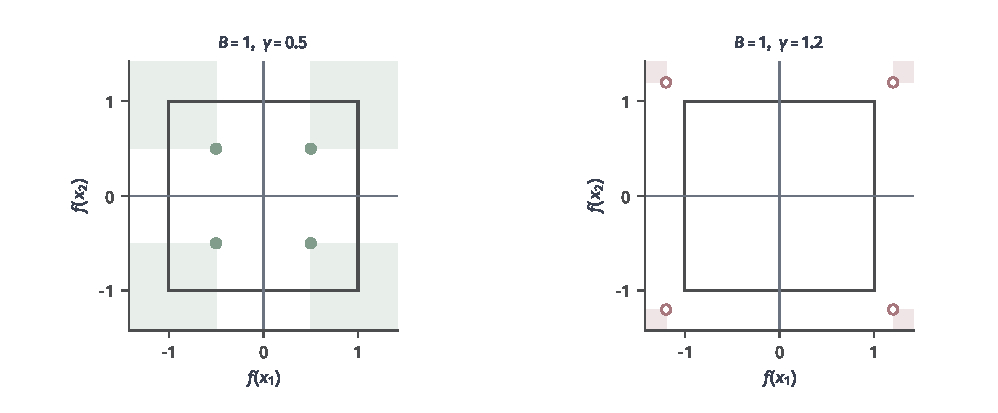
\includegraphics[width=164.6mm]{figures/06-foundations/02-learning-theory/matplotlib/comb-fat-margin-output-square/figure.pdf}
  \caption{两个分块、$B=1$与固定阈值$r_1=r_2=0$的输出几何。灰框是函数类允许的$(f(x_1),f(x_2))\in[-1,1]^2$；浅色区域要求两坐标分别离阈值至少$\gamma$。左图的浅绿区域对应$\gamma=0.5$，四种符号可由实心点实现；右图的浅红区域对应$\gamma=1.2$，空心点只标出要求的边界，全部落在允许框之外，因而不是类中的函数输出。图为解析教学构造。}
 \label{fig:comb-fat-margin-output-square}
 \label{fig:fat-shattering-example}
\end{figure*}
风险估计只要求达到指定精度$\eta$，相应的容量也应在这个数值尺度上衡量：两个函数在每个点上的差异都小于精度时，没有必要区分。下面的定理表明，对取值于$[0,1]$的函数类，在允许所有概率分布时，一致收敛成立当且仅当每个正尺度的胖打散维都有限。取值于一般有界区间的函数可以先平移缩放到$[0,1]$。

\begin{theorem}[胖打散维与一致收敛]
\label{thm:fat-uniform-convergence}
设$(X,\mathcal A)$为可测空间，$\mathcal F$为非空的$[0,1]$值可测函数空间。假定存在可数子空间$\mathcal F_0\subseteq\mathcal F$，使每个$f\in\mathcal F$都是$\mathcal F_0$中某个函数序列的逐点极限。则以下两个命题等价：
\begin{enumerate}
 \item 对每个$\gamma>0$，$\operatorname{fat}_{\gamma}(\mathcal F)<\infty$。
 \item 对任意$\eta,\delta\in(0,1)$，存在整数$n_0=n_0(\mathcal F,\eta,\delta)$，使任意$X$上的概率分布$\mathcal P$和任意$n\geq n_0$均满足
 \[
 \mathbb P_{(x_1,\ldots,x_n)\sim\mathcal P^n}\!\left\{
 \sup_{f\in\mathcal F}
 \left|\frac1n\sum_{i=1}^n f(x_i)-\mathbb E_{x\sim\mathcal P}f(x)\right|
 >\eta\right\}\leq\delta.
 \]
\end{enumerate}
\end{theorem}

定理两边的量词要分别看清。维度条件要求对每个$\gamma>0$，该尺度下的胖打散维都有限，但不同$\gamma$对应的维度可以随$\gamma$减小而增大。收敛条件要求同一个$n_0$适用于所有分布。可数子空间$\mathcal F_0$用来处理上确界的可测性；$\mathcal F$本身可数时直接取$\mathcal F_0=\mathcal F$。有界性还保证逐点逼近的函数在期望上也逼近，于是可以用可数子空间控制概率事件。要把定理用于学习问题，只需把$X$换成观测空间$Z$、令$\mathcal F=\mathcal F_\ell$，并核对有界性和可测性条件。

这一等价刻画的经典形式见学习理论教材\scite{shalevshwartz2014}，更精细的一致收敛上界见\scite{colomboni2023fat}。本书只说明证明路径，完整证明所需的覆盖数组合估计不在此展开。充分性仍采用副样本的想法：用另一份独立样本代替总体，把问题化为$2n$个点上的比较。困难在于有限输入上不同的损失向量有无穷多个，不能像VC分析那样精确计数。做法是把彼此相差不足某个精度（例如$\eta/4$）的损失向量归为一组，每组用一个代表向量近似；所需代表的最少个数称为该精度下的覆盖数。胖打散维与覆盖数的关系，类似VC维与生长函数的关系：适当尺度的胖打散维有限时，覆盖数的对数至多与该维度乘以样本量对数的平方同阶，远小于样本量本身。对有限个代表向量应用集中不等式并取并集界，再加上近似带来的误差，就得到全部函数的偏差控制。必要性从某个正尺度上任意大的打散点集出发：打散点远多于样本量时，在这些点上取均匀分布，任意一份样本都只覆盖其中一小部分；打散允许在抽到与未抽到的点上分别取阈值两侧、相差至少$2\gamma$的值，总能找到经验平均与总体平均相差约$\gamma$量级的函数，统一偏差因而不趋于零。

回到学习问题，定理的适用范围有三处限制。第一，胖打散比伪打散要求更强，所以有限伪维是一致收敛的较强充分条件；衰减例子说明它不是必要条件。第二，有界损失不能省略：无界损失还需要尾部控制，否则单个固定决策的经验风险也可能收敛很慢。第三，等价性针对全部分布；若允许族$\mathfrak P$较小，有限胖打散维仍足以保证一致收敛，但反方向可能不成立，因为受限分布未必能让函数之间的差异全部表现出来。最重要的是，这里刻画的是一致收敛，不是可学习性。结合定理~\ref{thm:general-uniform-pac}，有限胖打散维加上近似经验最优就给出学习保证；但不能把维度刻画直接改称一般学习的必要条件。下一小节说明二者确实可以分离。

\subsection{可学习而不一致收敛}

检验反方向时，可以构造一个决策空间：其中有一个已知的好决策，另有许多决策会使经验评价严重失真。取$Z=\mathbb N$，$w_0$是一个特殊决策，每个有限集$C\subset\mathbb N$也是一个决策，损失定义为
\[
 \ell(w_0,z)=0,\qquad \ell(C,z)=\mathbb I\{z\notin C\}.
\]
$w_0$在任何观测上都没有损失；集合决策$C$只在观测不属于$C$时受罚。所有有限子集是可数的，因此这个损失类满足可数逼近条件。

\begin{theorem}[可学习性不推出一致收敛]
\label{thm:general-learning-without-uniform}
令可测观测空间为$(Z,2^Z)$，其中$Z=\mathbb N$；令可测决策空间为$\mathcal W=\{w_0\}\cup\{C:C\subset\mathbb N,\ C\text{有限}\}$及其幂集，并允许$Z$上的所有概率分布。定义可测且取值于$\{0,1\}$的损失
\[
 \ell(w_0,z)=0,\qquad
 \ell(C,z)=\mathbb I\{z\notin C\}.
\]
对每个$n\geq1$，确定性算法$A_n:Z^n\to\mathcal W$定义为$A_n(S)=w_0$。则$(A_n)_{n\geq1}$分布无关PAC学习该问题，但损失类$\{z\mapsto\ell(w,z):w\in\mathcal W\}$不满足分布无关的一致收敛。
\end{theorem}
\begin{proof}
始终输出$w_0$的算法在每个分布下都具有零期望风险，因此达到最优。另一方面，对每个样本量$n$，令$\mathcal P_n$为$\{1,\ldots,2n\}$上的均匀分布。对任何$S\sim\mathcal P_n^n$，记其出现过的观测构成的集合为$C_S$。由于$|C_S|\leq n$，有
\[
 \hat R_S(C_S)=0,\qquad R_{\mathcal P_n}(C_S)\geq\frac12.
\]
前者因为每个样本点都属于$C_S$，后者因为$C_S$至多覆盖$\mathcal P_n$支持集的一半。一致收敛要求同一个样本量适用于所有分布，但每个$n$都有上述$\mathcal P_n$使统一偏差以概率1至少为$1/2$，所以分布无关的一致收敛不成立。
\end{proof}

在这个决策空间中，始终输出$w_0$和输出$C_S$的两个算法，经验风险都是0，因而都是ERM。但在证明使用的分布$\mathcal P_n$下，前者的期望风险为0，后者至少为$1/2$。经验最优只规定选择经验风险最小的决策，没有规定在多个并列最优者中如何选择，而这里的选择方式足以决定学习成败。成功的算法可以保留整个决策空间，不需要删去那些风险估计失真的集合决策。

这个构造并不否定二分类基本定理，因为二分类损失的结构不允许出现$w_0$这样的决策。二分类观测是$z=(x,y)$，损失由预测类别与标签是否相等决定：对同一个输入$x$，同一个分类器在$(x,0)$和$(x,1)$上不可能都取得零损失。这里的$w_0$却对全部观测零损失。分离也不来自损失的连续性或凸性：本例的损失只取0和1，与零一损失一样离散；起作用的是决策空间的结构，即同时存在一个处处零损失的决策和大量能贴合任意样本的集合决策。因此后续分析分成两类。复杂度方法仍控制整个损失类，只是改用依赖样本的度量。另外三种方法进一步利用实际算法的性质：样本压缩考察输出能否由少数训练记录重构，信息方法考察输出透露了多少样本信息，稳定性考察改变一条观测后损失或输出分布变化多少。对上述算法，输出恒为$w_0$：它不读取任何训练记录，不含样本信息，替换任何训练观测也不改变它；第~\ref{sec:algorithmic-stability}节的稳定性分析会直接给出学习保证，那些难以估计的集合决策与它无关。
\section{泛化分析工具}
\label{sec:generalization-tools}

用一份数据选模型，再用同一份数据报告成绩，成绩会偏乐观。看一个能完全算清的例子。设二元标签由公平硬币独立产生，输入不起作用，只比较恒预测0的分类器$h_0$与恒预测1的分类器$h_1$，二者的总体错误率都是$1/2$。用三条训练标签选择训练错误较少者：标签中1占多数就选$h_1$，否则选$h_0$，选中者的训练错误率因此至多为$1/3$。表~\ref{tab:lt7-selection-bias-coins}按标签分组列出全部8种情形：三条标签全相同时（概率合计$1/4$）训练错误为0，其余情形为$1/3$，所以平均训练错误为$\frac34\times\frac13=\frac14$。被选中分类器的总体错误率仍是$1/2$。模型的真实能力没有提高，训练成绩却因选择平均低估了$1/4$。

\begin{table}[htbp]
 \centering
 \footnotesize
 \begin{tabular}{@{}l c c c c@{}}
  \toprule
  \textbf{标签$(y_1,y_2,y_3)$} & \textbf{概率} & \textbf{选中} & \textbf{训练错误率} & \textbf{总体错误率} \\
  \midrule
  $000$ & $1/8$ & $h_0$ & $0$ & $1/2$ \\
  $001,\ 010,\ 100$ & $3/8$ & $h_0$ & $1/3$ & $1/2$ \\
  $011,\ 101,\ 110$ & $3/8$ & $h_1$ & $1/3$ & $1/2$ \\
  $111$ & $1/8$ & $h_1$ & $0$ & $1/2$ \\
  \midrule
  按概率平均 & & & $1/4$ & $1/2$ \\
  \bottomrule
 \end{tabular}
 \caption{选择造成的评价偏差。标签为独立的公平硬币，在两个常值分类器中按三条训练标签选择错误较少者。选中者的总体错误率恒为$1/2$，平均训练错误率只有$1/4$；若事先固定$h_0$，三条标签中1的平均个数为$3/2$，训练错误率的平均就是$1/2$。数值为教学构造，可逐行复算。}
 \label{tab:lt7-selection-bias-coins}
\end{table}

这个例子指出需要控制的是选后评价的偏差。对于抽样前已经固定的模型，独立同分布样本上的平均损失是总体风险的无偏估计；模型由同一份样本选出后，它与样本不再独立，不能再当作固定对象。本节的工具分别限制这种选择所能利用的随机波动：数据依赖的复杂度考察整个函数类顺应噪声的能力，样本压缩考察输出能否由少数记录重构，信息量考察输出透露了多少样本信息，稳定性考察单个观测对结果的影响。

四条路线依次展开：先从随机噪声拟合进入复杂度，再从少量记录重构进入压缩，随后把选择代价写成信息量，最后通过替换观测解释稳定性。复杂度与压缩最终仍对一组候选同时控制偏差，信息与稳定性直接分析算法输出的分布或变化；第~\ref{sec:stability-comparison}节比较后三者控制的对象及其联系。每条路线都要说明怎样把它控制的量接到经验风险与总体风险之差，结论可能是期望保证，也可能是高概率保证，按各自条件分别建立。它们回答的都是“经验评价是否可信”；统计偏差小以后，还需要经验拟合或优化误差小，才能得到完整的学习保证，这一项由第~\ref{sec:risk-comparison}节的风险比较另行计入。

\subsection{数据依赖的复杂度}
\label{sec:rademacher-complexity}

固定一份样本，在每个位置放上独立的随机正负号，再允许从函数类中挑选与这些符号最一致的函数。这些符号没有任何可推广的规律；一个函数类若仍能大幅迎合它们，仅凭样本上的拟合成绩就很难区分规律与偶然波动。Rademacher复杂度衡量这种迎合能力，高斯复杂度把等幅的正负号换成随机振幅，为同一问题提供另一种计算方式。这些辅助随机变量只用于分析，不要求真的打乱标签后重新训练。

与VC界相比，这样做利用了实际样本。VC补偿项只依赖VC维，而VC维按最不利的输入位置计算：即使样本集中在一个小区域、函数类在那里只能给出很少几种预测，补偿项也不变小。随机噪声为什么与泛化有关，要在第~\ref{sec:rademacher-symmetrization-bound}节建立桥梁：用另一份独立样本代表总体表现，两份样本的损失差经随机交换变成带正负号的和，正是这里度量的量。第~\ref{sec:binary-learnability-characterization}节的对称化证明在交换观测后需要控制的也是它，只是那里先在最坏输入上数出预测模式，再用并集界上界它。下面先定义两种复杂度，再建立运算性质，然后推导风险界，最后计算线性与核函数类；模型选择与集成学习中的应用分别在第~\ref{sec:srm}节、第~\ref{sec:boosting}节。

\subsubsection{Rademacher复杂度}

先看一个能逐项算出的例子。图~\ref{fig:lt7a-rademacher-noise-fit}中的函数类只有三个函数，在5个样本点上的取值都是$\pm1$。给每个样本点独立分配一个等概率取$\pm1$的符号$\sigma_i$，把它看作毫无规律的噪声标签。对一串符号$\bm\sigma$，函数$f$与噪声的吻合程度用内积$\langle\bm\sigma,f\rangle=\sum_i\sigma_if(z_i)$衡量：取值一致的位置贡献$+1$，不一致的贡献$-1$。函数类“追随噪声”的能力，就是在类中挑出与这串符号最吻合的函数。符号$\bm\sigma^{(a)}=(+,-,-,+,+)$下，三个内积为$1,1,-5$，最大值为$1$；符号$\bm\sigma^{(b)}=(+,+,-,-,-)$下，内积为$-1,3,1$，$f_2$与之最吻合，最大值为$3$。把最大内积除以样本量，再对全部$2^5=32$串符号平均，枚举得到$0.4$。

\begin{figure}[htbp]
 \centering
 % 函数类追随随机符号：三个函数在5个样本点上的取值与两串随机符号的内积。
% 数据：f1=(1,1,1,1,1), f2=(1,1,-1,-1,1), f3=(-1,1,1,-1,-1)；
% sigma^(a)=(+,-,-,+,+) 给出内积 (1,1,-5)，最大值1；
% sigma^(b)=(+,+,-,-,-) 给出内积 (-1,3,1)，最大值3。
% 对全部32串符号平均 max_j <sigma,f_j>/5 得 0.4（枚举复算）。
\begingroup
\providecolor{FigureGreen}{HTML}{829C8B}
\providecolor{FigureGreenFill}{HTML}{E8EEE9}
\begin{tikzpicture}[figure picture,x=1mm,y=1mm]
\def\cw{9}\def\ch{6}
% 列标题
\foreach \i in {1,...,5}{\node[figure note] at ({18+\i*\cw},47) {$z_{\i}$};}
\node[figure note] at (82,47) {$\langle\bm\sigma^{(a)},f\rangle$};
\node[figure note] at (101,47) {$\langle\bm\sigma^{(b)},f\rangle$};
% 函数行
\def\rowf#1#2#3{%
 \node[anchor=east] at (24,#1) {$#2$};
 \foreach \v [count=\i] in {#3}{%
  \ifnum\v>0
   \filldraw[draw=FigureBlue,fill=FigureBlueFill,line width=.5pt] ({18+\i*\cw-\cw/2+.6},{#1-\ch/2+.6}) rectangle ({18+\i*\cw+\cw/2-.6},{#1+\ch/2-.6});
   \node[text=FigureBlue] at ({18+\i*\cw},#1) {$+1$};
  \else
   \filldraw[draw=FigureRed,fill=FigureRedFill,line width=.5pt] ({18+\i*\cw-\cw/2+.6},{#1-\ch/2+.6}) rectangle ({18+\i*\cw+\cw/2-.6},{#1+\ch/2-.6});
   \node[text=FigureRed] at ({18+\i*\cw},#1) {$-1$};
  \fi}}
\rowf{40}{f_1}{1,1,1,1,1}
\rowf{33}{f_2}{1,1,-1,-1,1}
\rowf{26}{f_3}{-1,1,1,-1,-1}
% 内积列
\node at (82,40) {$1$};\node at (82,33) {$1$};\node at (82,26) {$-5$};
\node at (101,40) {$-1$};\node at (101,26) {$1$};
\draw[FigureGreen,line width=.9pt,rounded corners=1mm] (96.5,30.2) rectangle (105.5,35.8);
\node at (101,33) {$3$};
\draw[FigureGreen,line width=.9pt,rounded corners=1mm] (77.5,37.2) rectangle (86.5,42.8);
\draw[FigureGreen,line width=.9pt,rounded corners=1mm] (77.5,30.2) rectangle (86.5,35.8);
\draw[FigureGrid,line width=.5pt] (20,21.5)--(108,21.5);
% 符号行
\def\rows#1#2#3{%
 \node[anchor=east] at (24,#1) {$#2$};
 \foreach \v [count=\i] in {#3}{%
  \filldraw[draw=FigureYellow,fill=FigureYellowFill,line width=.5pt] ({18+\i*\cw-\cw/2+.6},{#1-\ch/2+.6}) rectangle ({18+\i*\cw+\cw/2-.6},{#1+\ch/2-.6});
  \node at ({18+\i*\cw},#1) {$\v$};}}
\rows{16}{\bm\sigma^{(a)}}{+,-,-,+,+}
\rows{9}{\bm\sigma^{(b)}}{+,+,-,-,-}
\node[figure note,anchor=west] at (72,16) {最大内积 $1$，贡献 $1/5$};
\node[figure note,anchor=west] at (72,9) {最大内积 $3$，贡献 $3/5$};
\node[figure note] at (64,1.5) {对全部 $2^5=32$ 串符号平均：$\widehat{\mathfrak R}_S=0.4$};
\end{tikzpicture}
\endgroup

 \caption{函数类追随随机符号的能力。上方三行是三个函数在5个样本点上的取值（蓝为$+1$、红为$-1$），下方两行是两串随机符号；右侧两列是每个函数与对应符号串的内积，绿框标出类中最大者。对全部32串符号平均“最大内积除以5”，得到这一类在该样本上的经验Rademacher复杂度$0.4$。数值为教学构造，可逐项复算。}
 \label{fig:lt7a-rademacher-noise-fit}
\end{figure}

这个平均就是下面定义的量。计算顺序很关键：先固定一串符号、在函数类上取上确界，再对符号取平均。函数可以随符号改变，这正是要测的拟合自由度；若先平均再取上确界，每个函数的平均相关和都是零，便什么也测不到。由于后面需要控制的是经验均值低于总体均值的程度，正文采用不带绝对值的单侧版本；后面若用到绝对值版本，会单独说明转换。

\begin{definition}[Rademacher复杂度]
\label{def:learning-rademacher-complexity}
设$\mathcal G$为从$Z$到$\mathbb R$的非空函数类，$S=(z_1,\ldots,z_n)$为一份样本，$\sigma_1,\ldots,\sigma_n$相互独立、等概率取$-1$和$1$，并独立于$S$。称
\begin{equation}
 \widehat{\mathfrak R}_S(\mathcal G)
 =\mathbb E_\sigma\left[\sup_{f\in\mathcal G}
       \frac1n\sum_{i=1}^n\sigma_i f(z_i)\right]
 \label{eq:learning-empirical-rademacher}
\end{equation}
为$\mathcal G$在$S$上的经验\term{Rademacher复杂度}（Rademacher complexity）。对$S\sim\mathcal P^n$再取期望，得到总体版本$\mathfrak R_n(\mathcal G)=\mathbb E_{S\sim\mathcal P^n}\widehat{\mathfrak R}_S(\mathcal G)$。涉及上确界时，假定$\mathcal G$有可数逼近子类，使上确界可测。
\end{definition}

经验版本依赖这一份样本，只要算出函数类在样本点上的取值向量集合$\mathcal G|_S=\{(f(z_1),\ldots,f(z_n)):f\in\mathcal G\}$即可计算；总体版本依赖抽样分布，是对样本取平均后的量。两个极端情形说明数值的含义。若$\mathcal G$只含一个函数，上确界不起作用，而$\mathbb E\sigma_i=0$，正负号平均抵消，复杂度为零：一个事先固定的函数无法追随噪声。复杂度为零并不表示有限样本误差为零，这个函数的经验风险仍会随抽样波动，那部分由第~\ref{sec:rademacher-symmetrization-bound}节风险界中的集中项控制。若$\mathcal G$取值于$\{0,1\}$且在样本上实现全部$2^n$种取值向量，即样本被打散，那么对每串符号都可以选在$\sigma_i=1$处取1、其余处取0的函数，上确界等于正号所占比例，复杂度为$1/2$，这是$[0,1]$值函数类能达到的最大值。对图中的$\pm1$值函数，若类包含全部32种取值向量，每串符号都能被完全复制，复杂度为$1$；只含三个函数时为$0.4$。

常见的另一种定义在上确界内取绝对值，它等于$\mathcal G\cup(-\mathcal G)$的单侧复杂度。图中三函数类加入各自的相反函数后，单侧复杂度从$0.4$升到$0.6$：符号$\bm\sigma^{(a)}$下，$-f_3$与之完全一致，内积为$5$。对取负封闭的函数类，两种定义相同；一般情况下，带绝对值的版本不小于单侧版本。后面的收缩引理和比较结果的常数依赖所用版本，引用外部结论时要核对约定，不能混用。

介于两极端之间时，复杂度由函数类在样本上实际能取到多少种值、这些值有多大决定。零一损失下，取值向量至多$\Pi_{\mathcal H}(n)$种，第~\ref{sec:comb-vc-growth}节的计数因而可以直接转化为复杂度的上界，这一联系在第~\ref{sec:rademacher-operations}节由Massart引理给出。计数保留的是“有几种”，复杂度还保留了“取值多大、彼此多远”，因此能够用于实值损失；风险保证在第~\ref{sec:rademacher-symmetrization-bound}节统一推导。
\subsubsection{高斯复杂度}

沿用前面的随机配合实验，把每个位置的等幅正负号换成标准高斯变量：方向仍是随机的，振幅也有了大小。保持样本、函数类和归一化不变，只改变辅助随机过程，就得到另一种衡量函数类拟合噪声能力的量。引入它的理由在计算：高斯变量的线性组合仍是高斯变量，二阶矩便于处理线性函数与范数约束，还可以使用高斯过程的比较不等式等专门工具。它不是另一种学习任务，也不另起一套风险分析主线。

\begin{definition}[高斯复杂度]
\label{def:learning-gaussian-complexity}
在定义~\ref{def:learning-rademacher-complexity}的设定下，令$\xi_1,\ldots,\xi_n$为独立于$S$的独立标准高斯变量。称
\[
 \widehat{\mathfrak G}_S(\mathcal G)
 =\mathbb E_\xi\left[\sup_{f\in\mathcal G}\frac1n\sum_{i=1}^n \xi_i f(z_i)\right]
\]
为$\mathcal G$在$S$上的单侧\term{经验高斯复杂度}（empirical Gaussian complexity）。
\end{definition}

两种噪声的差别在幅度：Rademacher符号的幅度恒为1，高斯变量的幅度$|\xi_i|$随机变化，平均为$\mathbb E|\xi_i|=\sqrt{2/\pi}\approx0.80$，偶尔很大。图~\ref{fig:lt7a-gaussian-rademacher}左侧画出一组$|\sigma_i|$与$|\xi_i|$。函数类若能在单个坐标上“押注”，高斯噪声中偶然出现的大幅度就会被上确界捕获。下面的比较说明一个方向总成立。

\begin{lemma}[高斯复杂度控制Rademacher复杂度]
\label{lem:gaussian-rademacher-comparison}
在上述设定下，若两种复杂度有限，则$\widehat{\mathfrak G}_S(\mathcal G)\geq\sqrt{2/\pi}\,\widehat{\mathfrak R}_S(\mathcal G)$。
\end{lemma}
\begin{proof}
把$\xi_i$写成$\sigma_i|\xi_i|$。标准高斯分布关于零对称，故$\sigma_i=\operatorname{sign}\xi_i$等概率取$\pm1$，且与$|\xi_i|$独立。固定$\bm\sigma$后对$|\xi|$取期望，函数$\bm a\mapsto\sup_f\frac1n\sum_i\sigma_ia_if(z_i)$是一族线性函数的上确界，因而是凸函数；Jensen不等式给出
\[
\begin{aligned}
 \mathbb E_{|\xi|}\sup_f\frac1n\sum_i\sigma_i|\xi_i|f(z_i)
 &\geq\sup_f\frac1n\sum_i\sigma_i\,\mathbb E|\xi_i|\,f(z_i)\\
 &=\sqrt{\frac2\pi}\sup_f\frac1n\sum_i\sigma_if(z_i).
\end{aligned}
\]
再对$\bm\sigma$取期望即得结论。
\end{proof}

因此，已知高斯复杂度的上界$b(S)$时，$\sqrt{\pi/2}\,b(S)$就是Rademacher复杂度的上界，可以代入后面的风险界。反方向一般不能用与$n$无关的常数比较。设函数在固定样本上的取值向量只有$\{\pm\bm e_i:1\leq i\leq n\}$这$2n$个，其中$\bm e_i$是第$i$个坐标向量。此时$\sup_f\sum_i\sigma_if(z_i)=\max_i|\sigma_i|=1$，经验Rademacher复杂度为$1/n$；同理经验高斯复杂度为$\mathbb E\max_i|\xi_i|/n$。图~\ref{fig:lt7a-gaussian-rademacher}右侧用数值积分$\mathbb E\max_i|\xi_i|=\int_0^\infty[1-(2\Phi(t)-1)^n]\,\mathrm dt$算出后者：$n=1$时为$0.80$，$n=10$时为$1.88$，$n=1000$时为$3.44$，与$\sqrt{2\log(2n)}$同阶增长。这个例子中的函数取负值，不能直接套用后面关于$[0,1]$值损失的风险定理；它只说明替换复杂度时必须核对比较的方向和常数因子。

\begin{figure*}[htbp]
 \centering
 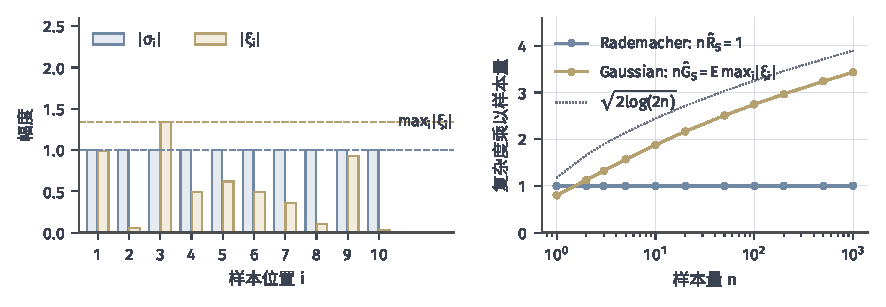
\includegraphics[width=150mm]{figures/06-foundations/02-learning-theory/matplotlib/lt7a-gaussian-rademacher/figure.pdf}
 \caption{高斯噪声与Rademacher噪声的对照。左：10个位置上随机符号的幅度恒为1（蓝），一组标准高斯变量的幅度（黄，随机种子7）有大有小，虚线标出各自的最大值。右：取值向量为$\{\pm\bm e_i\}$的函数类，$n$倍经验Rademacher复杂度恒为1，$n$倍经验高斯复杂度等于$\mathbb E\max_i|\xi_i|$（数值积分），随$n$按$\sqrt{2\log(2n)}$（点线）的量级增长。}
 \label{fig:lt7a-gaussian-rademacher}
\end{figure*}

\subsubsection{复杂度的运算性质}
\label{sec:rademacher-operations}

直接按定义计算复杂度往往困难。下面几条规则把复杂的类归约为简单的类。它们都只依赖函数类在样本上的取值向量集合，所以统一对固定样本陈述；对样本取期望后同样适用于总体版本。所涉及的上确界与期望按定义~\ref{def:learning-rademacher-complexity}的可数逼近约定理解。

\begin{lemma}[缩放、平移与求和]
\label{lem:rademacher-basic-operations}
固定样本$S$。对非空函数类$\mathcal G,\mathcal G'$、常数$c\in\mathbb R$及固定函数$g_0$，有：
\begin{enumerate}
 \item $\widehat{\mathfrak R}_S(c\,\mathcal G)=|c|\,\widehat{\mathfrak R}_S(\mathcal G)$；
 \item $\widehat{\mathfrak R}_S(\mathcal G+g_0)=\widehat{\mathfrak R}_S(\mathcal G)$，其中$\mathcal G+g_0=\{f+g_0:f\in\mathcal G\}$；
 \item $\mathcal G\subseteq\mathcal G'$时$\widehat{\mathfrak R}_S(\mathcal G)\leq\widehat{\mathfrak R}_S(\mathcal G')$；
 \item $\widehat{\mathfrak R}_S(\mathcal G+\mathcal G')\leq\widehat{\mathfrak R}_S(\mathcal G)+\widehat{\mathfrak R}_S(\mathcal G')$，其中$\mathcal G+\mathcal G'=\{f+f':f\in\mathcal G,f'\in\mathcal G'\}$。
\end{enumerate}
\end{lemma}
\begin{proof}
第一条：$c\geq0$时常数可提出上确界；$c<0$时，$\sum_i\sigma_icf(z_i)=|c|\sum_i(-\sigma_i)f(z_i)$，而$-\bm\sigma$与$\bm\sigma$同分布。第二条：$\sum_i\sigma_ig_0(z_i)$不依赖$f$，可移出上确界，而它的期望为零。第三条：在更大的集合上取上确界不会变小。第四条：$\sup_{f,f'}(a_f+b_{f'})=\sup_fa_f+\sup_{f'}b_{f'}$，再取期望。
\end{proof}

第一条说明，单独把类取负不改变单侧复杂度：图~\ref{fig:lt7a-rademacher-noise-fit}中的$\{-f_1,-f_2,-f_3\}$复杂度仍为$0.4$。前面从$0.4$升到$0.6$，是因为把$\mathcal G$与$-\mathcal G$并在一起，类变大了；这正是第三条的单调性。第二条说明，把损失减去一个固定基准不改变复杂度，这在收缩引理中会用到。
有限函数类的复杂度可以由计数和取值大小控制，这把第~\ref{sec:binary-shattering-vc}节的组合计数接到数值复杂度上。

\begin{lemma}[Massart引理]
\label{lem:rademacher-massart}
设有限集合$T\subset\mathbb R^n$含$N\geq1$个向量，且每个$\bm t\in T$满足$\|\bm t\|_2\leq r_0$。则
\[
 \mathbb E_\sigma\max_{\bm t\in T}\frac1n\sum_{i=1}^n\sigma_it_i
 \leq\frac{r_0\sqrt{2\log N}}{n}.
\]
特别地，若函数类在样本$S$上只有$N$种取值向量且它们的欧氏范数至多为$r_0$，则$\widehat{\mathfrak R}_S(\mathcal G)\leq r_0\sqrt{2\log N}/n$。
\end{lemma}
\begin{proof}
$N=1$时左侧为零。设$N\geq2$，任取$\lambda>0$。由Jensen不等式，再把最大值放大为求和，
\[
 e^{\lambda\,\mathbb E\max_{\bm t}\langle\bm\sigma,\bm t\rangle}
 \leq\mathbb E e^{\lambda\max_{\bm t}\langle\bm\sigma,\bm t\rangle}
 \leq\sum_{\bm t\in T}\prod_{i=1}^n\mathbb E e^{\lambda\sigma_it_i}
 =\sum_{\bm t\in T}\prod_{i=1}^n\cosh(\lambda t_i).
\]
由$\cosh u\leq e^{u^2/2}$，右侧至多$Ne^{\lambda^2r_0^2/2}$。取对数得$\mathbb E\max_{\bm t}\langle\bm\sigma,\bm t\rangle\leq\log N/\lambda+\lambda r_0^2/2$；取$\lambda=\sqrt{2\log N}/r_0$使两项相等，即得$r_0\sqrt{2\log N}$，再除以$n$。
\end{proof}

对图~\ref{fig:lt7a-rademacher-noise-fit}的三函数类，$N=3$、$r_0=\sqrt5$，引理给出$\sqrt5\sqrt{2\log3}/5\approx0.66$，确实不小于枚举值$0.4$。对取值于$\{0,1\}$的零一损失类，$r_0\leq\sqrt n$；固定标签后，损失向量与预测向量一一对应，$N\leq\Pi_{\mathcal H}(n)$。结合Sauer--Shelah引理~\ref{lem:sauer-shelah}，当$1\leq d=\operatorname{VC}(\mathcal H)\leq n$时，
\begin{equation}
 \widehat{\mathfrak R}_S(\mathcal G)\leq\sqrt{\frac{2\log\Pi_{\mathcal H}(n)}{n}}\leq\sqrt{\frac{2d\log(en/d)}{n}}.
 \label{eq:rademacher-vc-comparison}
\end{equation}
所以Rademacher复杂度至多与VC界同阶；样本上实际出现的预测模式少于最坏情形时，它还会更小。

预测函数类的复杂度往往容易计算，风险却由损失值决定：风险评价对损失类取平均，不能只计算预测函数的复杂度。若损失对得分是$L$-Lipschitz的，得分变化$\Delta$造成的损失变化至多$L\Delta$，损失类迎合随机符号的能力就不应超过得分类的$L$倍。下面的\term{收缩引理}（contraction lemma）把这一直觉精确化。

\begin{lemma}[收缩引理]
\label{lem:rademacher-contraction}
设$T\subset\mathbb R^n$为非空有界集合，$\phi_1,\ldots,\phi_n:\mathbb R\to\mathbb R$都是$L$-Lipschitz函数，即$|\phi_i(u)-\phi_i(u')|\leq L|u-u'|$。则
\[
 \mathbb E_\sigma\sup_{\bm t\in T}\sum_{i=1}^n\sigma_i\phi_i(t_i)
 \leq L\,\mathbb E_\sigma\sup_{\bm t\in T}\sum_{i=1}^n\sigma_it_i.
\]
\end{lemma}
\begin{proof}
逐个坐标把$\phi_i(t_i)$换成$Lt_i$。先处理第一个坐标：固定$\sigma_2,\ldots,\sigma_n$，记$A(\bm t)=\sum_{i\geq2}\sigma_i\phi_i(t_i)$。对$\sigma_1$的两个取值求平均，并把两个上确界合并为对一对$(\bm t,\bm t')$的上确界：
\[
 \mathbb E_{\sigma_1}\sup_{\bm t}\bigl[\sigma_1\phi_1(t_1)+A(\bm t)\bigr]
 =\frac12\sup_{\bm t,\bm t'}\bigl[\phi_1(t_1)-\phi_1(t_1')+A(\bm t)+A(\bm t')\bigr].
\]
由Lipschitz条件，方括号至多$L|t_1-t_1'|+A(\bm t)+A(\bm t')$。后两项关于交换$\bm t,\bm t'$对称，所以在上确界中总可以让$t_1\geq t_1'$，绝对值可以去掉：
\[
 \frac12\sup_{\bm t,\bm t'}\bigl[L t_1-Lt_1'+A(\bm t)+A(\bm t')\bigr]
 =\mathbb E_{\sigma_1}\sup_{\bm t}\bigl[\sigma_1Lt_1+A(\bm t)\bigr].
\]
再对$\sigma_2,\ldots,\sigma_n$取期望，就把第一个坐标换成了$Lt_1$。对第$k$个坐标重复同一论证，此时$A$中前$k-1$项已是$\sigma_iLt_i$，其余仍是$\sigma_i\phi_i(t_i)$，论证不受影响。$T$有界保证所有上确界有限。
\end{proof}

证明的关键一步是：两个得分相差$|t_1-t_1'|$时，经过$\phi_1$后至多相差$L|t_1-t_1'|$，所以“在单个坐标上押注的收益”不会变大。图~\ref{fig:lt7a-contraction-geometry}画出这一几何：左侧的间隔损失斜率至多$1/\rho$，两对得分经过它后的差距不超过原差距的$1/\rho$倍，在平坦段甚至变为零；右侧把两个样本点上的得分向量逐坐标作用损失，得到的点集在每个坐标方向上都不比原来更宽。应用于学习时，固定标签$y_i$，令$\phi_i(u)=\ell(u,y_i)$，取$T$为得分类$\mathcal F$在样本上的取值向量集合：若损失对得分是$L$-Lipschitz的，损失类$\ell\circ\mathcal F$的经验复杂度至多为$L\,\widehat{\mathfrak R}_S(\mathcal F)$，这里$\widehat{\mathfrak R}_S(\mathcal F)$只需在输入上计算。单侧版本不要求$\phi_i(0)=0$；带绝对值的版本通常要求这一点，且常数可能多出因子2，两种口径不能混用。零一损失在阈值处跳变，不满足Lipschitz条件，不能直接收缩，需要先换成第~\ref{sec:rademacher-symmetrization-bound}节的间隔损失。

\begin{figure*}[htbp]
 \centering
 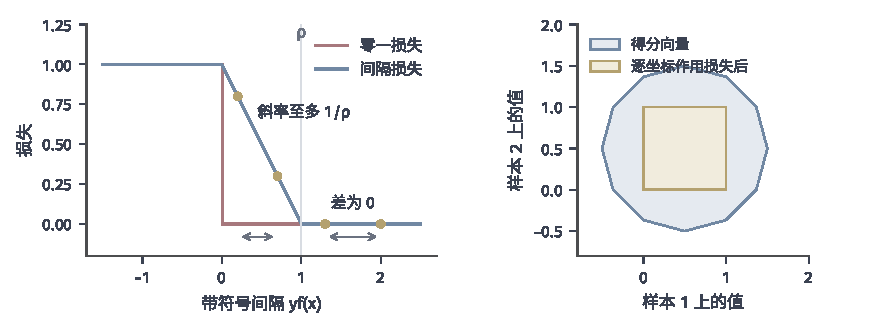
\includegraphics[width=150mm]{figures/06-foundations/02-learning-theory/matplotlib/lt7a-contraction-geometry/figure.pdf}
 \caption{收缩引理的Lipschitz几何（$\rho=1$）。左：间隔损失$\ell_\rho$在$0<yf<\rho$处斜率为$-1/\rho$，其余处平坦，处处不小于零一损失；两对得分（黄点）经过它后的差距不超过得分差的$1/\rho$倍，右侧一对的差变为零。右：两个样本点上的12个得分向量（蓝，圆心$(0.5,0.5)$、半径1的圆上取点）逐坐标作用$\ell_\rho$后（黄）被压进$[0,1]^2$，灰线连接对应点。图为解析教学构造。}
 \label{fig:lt7a-contraction-geometry}
\end{figure*}

最后一条性质处理加权平均。集成方法把多个基函数按非负、和为1的权重组合，组合后的函数似乎更灵活，复杂度却不变。原因是一个简单事实：若干数的凸组合不会超过其中的最大值。固定随机符号后，凸组合函数与符号的相关和，正是各成员相关和的同一凸组合。

\begin{lemma}[凸包不增加Rademacher复杂度]
\label{lem:rademacher-convex-hull}
固定样本$S$与非空实值函数类$\mathcal B$，令$\operatorname{conv}(\mathcal B)$为$\mathcal B$中有限个函数的全部凸组合$\sum_ja_jh_j$（$a_j\geq0$，$\sum_ja_j=1$）。若$\widehat{\mathfrak R}_S(\mathcal B)$有限，则
\[
 \widehat{\mathfrak R}_S(\operatorname{conv}(\mathcal B))=\widehat{\mathfrak R}_S(\mathcal B).
\]
进一步，对带符号组合$\{\sum_ja_jh_j:h_j\in\mathcal B,\ \sum_j|a_j|\leq1\}$，复杂度等于$\widehat{\mathfrak R}_S(\mathcal B\cup-\mathcal B\cup\{0\})$。
\end{lemma}
\begin{proof}
固定$\bm\sigma$，映射$f\mapsto\sum_i\sigma_if(z_i)$是线性的，于是
\[
 \sum_i\sigma_i\sum_ja_jh_j(z_i)=\sum_ja_j\sum_i\sigma_ih_j(z_i)\leq\sup_{h\in\mathcal B}\sum_i\sigma_ih(z_i).
\]
凸组合的上确界因此不超过$\mathcal B$上的上确界，而$\mathcal B\subseteq\operatorname{conv}(\mathcal B)$给出反向不等式；对$\bm\sigma$取期望即得等式。带符号组合可写成$\mathcal B\cup-\mathcal B\cup\{0\}$的凸组合，同理可得。
\end{proof}

这条性质控制的是归一化得分的复杂度，不是取符号后投票分类器的复杂度；零一损失仍须先经间隔损失连接。它不涉及成员个数，所以对无限基函数类同样成立。第~\ref{sec:boosting}节在加权投票的间隔分析中使用它。
\subsubsection{对称化与风险界}
\label{sec:rademacher-symmetrization-bound}

现在把复杂度接到风险上。设损失取值于$[0,1]$，决策$w$对应损失函数$g_w=\ell(w,\cdot)$，它们组成损失类$\mathcal G$。$g_w$在样本上的均值是经验风险，在总体上的均值是期望风险。算法会挑训练表现好的函数，所以这条路线不追踪算法，而是先对整个损失类控制“总体均值减经验均值”的上确界；这个上确界受控以后，最后代入算法实际选出的决策即可。

\begin{theorem}[Rademacher复杂度给出的期望风险上界]
\label{thm:rademacher-risk-bound}
设$(Z,\mathcal A)$为可测空间，$\mathcal P$为$Z$上的概率分布，$n\geq1$，$S=(z_1,\ldots,z_n)\sim\mathcal P^n$。令$\mathcal G$为抽样前确定的、从$Z$到$[0,1]$的非空可测函数空间，并存在可数子类$\mathcal G_0\subseteq\mathcal G$，使$\mathcal G$中的每个函数都是$\mathcal G_0$中某个函数序列的逐点极限。则对任意$\delta\in(0,1)$，以关于$S$至少$1-\delta$的概率，所有$g\in\mathcal G$同时满足
\begin{equation}
 \mathbb E_{z\sim\mathcal P}g(z)
 \leq\frac1n\sum_i g(z_i)+2\mathfrak R_n(\mathcal G)
 +\sqrt{\frac{\log(1/\delta)}{2n}}.
 \label{eq:rademacher-risk-bound}
\end{equation}
另有一个由样本确定的上界：以至少$1-\delta$的概率，所有$g\in\mathcal G$同时满足
\begin{equation}
 \mathbb E_{z\sim\mathcal P}g(z)
 \leq\frac1n\sum_i g(z_i)+2\widehat{\mathfrak R}_S(\mathcal G)
 +3\sqrt{\frac{\log(2/\delta)}{2n}}.
 \label{eq:empirical-rademacher-risk-bound}
\end{equation}
\end{theorem}

证明按“总体与经验之差—两份样本之差—随机符号过程—统一风险界”四步展开。第一步引入一份独立同分布的副样本：对固定函数，副样本上的平均损失在取期望后等于总体风险，于是未知总体均值的单侧偏差可以归约为两份样本平均损失之差的上确界。这里只用期望关系，不把一份有限副样本直接等同于总体。第二步对每一对训练观测与副样本观测随机决定是否交换位置。图~\ref{fig:lt7-symmetrization-swap}固定一个函数演示交换：交换不改变两份样本的联合分布，却让该位置的差恰好乘上一个随机符号，两份样本之差因而变成带随机符号的和，第三步再用复杂度控制它。第四步用集中不等式说明最大偏差本身以高概率接近其期望。

\begin{figure}[htbp]
 \centering
 % 对称化中的逐对交换（教学构造）。
% 固定一个损失函数 g，训练样本 S 的四个损失值 g(z_i)=0.2,0.7,0.1,0.9，
% 副样本 S' 的损失值 g(z_i')=0.6,0.3,0.5,0.4；差 d_i=g(z_i')-g(z_i)=+0.4,-0.4,+0.4,-0.5。
% 符号 sigma=(+1,-1,+1,-1)：在 sigma_i=-1 的第2、4列交换 z_i 与 z_i'，
% 交换后的差为 sigma_i d_i=+0.4,+0.4,+0.4,+0.5。交换不改变 (S,S') 的联合分布。
% 宽度约 105 mm。
\begingroup
\begin{tikzpicture}[figure picture,x=1mm,y=1mm]
\tikzset{cell/.style={rectangle,draw=FigureStroke,line width=.6pt,minimum width=16mm,minimum height=6.5mm,inner sep=1pt,font=\figurefont\footnotesize},
 swap/.style={{Stealth[length=1.6mm,width=1.1mm]}-{Stealth[length=1.6mm,width=1.1mm]},draw=FigureRed,line width=.8pt}}
\node[figure note,anchor=east] at (17,40) {符号 $\sigma_i$};
\node[figure note,anchor=east] at (17,30) {训练样本 $S$};
\node[figure note,anchor=east] at (17,14) {副样本 $S'$};
\node[figure note,anchor=east] at (17,3) {差 $d_i\to\sigma_id_i$};
\foreach \i/\x/\s/\a/\b/\d/\e in {1/28/+1/0.2/0.6/{+0.4}/{+0.4},2/50/-1/0.7/0.3/{-0.4}/{+0.4},3/72/+1/0.1/0.5/{+0.4}/{+0.4},4/94/-1/0.9/0.4/{-0.5}/{+0.5}}{
  \node[figure heading] at (\x,46) {$i=\i$};
  \node[font=\figurefont\footnotesize] at (\x,40) {$\s$};
  \node[cell,fill=FigureBlueFill] at (\x,30) {$g(z_\i)=\a$};
  \node[cell,fill=FigureYellowFill] at (\x,14) {$g(z_\i')=\b$};
  \node[font=\figurefont\footnotesize] at ({\x-4},3) {$\d$};
  \node[font=\figurefont\footnotesize,text=FigureRed] at ({\x+4},3) {$\to\e$};
}
\foreach \x in {50,94}{\draw[swap] ({\x-5},26.6) to[bend right=25] ({\x-5},17.4); \node[figure note,text=FigureRed] at ({\x+3},22) {交换};}
\foreach \x in {28,72}{\node[figure note] at (\x,22) {不动};}
\end{tikzpicture}
\endgroup

 \caption{对称化中的逐对交换。固定一个损失函数$g$，上行是训练样本上的损失值，下行是副样本上的损失值。符号为$-1$的第2、4列交换两份样本中的观测，差$d_i=g(z_i')-g(z_i)$随之变号，成为$\sigma_id_i$。两份样本独立同分布，交换前后的联合分布相同，所以$\sum_id_i$与$\sum_i\sigma_id_i$同分布；对整个函数类取上确界后，后者正由Rademacher复杂度控制。数值为教学构造。}
 \label{fig:lt7-symmetrization-swap}
\end{figure}

\begin{proof}
令$\Phi(S)=\sup_{g\in\mathcal G}(\mathbb E g-n^{-1}\sum_i g(z_i))$，即经验均值在整个类上的最大低估。取独立副样本$S'=(z_1',\ldots,z_n')\sim\mathcal P^n$，则$\mathbb E g=\mathbb E_{S'}\frac1n\sum_ig(z_i')$。对每个$g$先取期望再取上确界，不超过先取上确界再取期望，故
\[
 \mathbb E_S\Phi(S)
 \leq\mathbb E_{S,S'}\sup_{g\in\mathcal G}
 \frac1n\sum_i\bigl(g(z_i')-g(z_i)\bigr).
\]
对任意固定的$\bm\sigma\in\{\pm1\}^n$，在$\sigma_i=-1$的位置交换$z_i$与$z_i'$，不改变$(S,S')$的联合分布，而差值$g(z_i')-g(z_i)$恰好变号。所以右侧等于
\[
\begin{aligned}
 &\mathbb E_{\sigma,S,S'}\sup_{g}\frac1n\sum_i\sigma_i\bigl(g(z_i')-g(z_i)\bigr)\\
 &\quad\leq\mathbb E\sup_g\frac1n\sum_i\sigma_ig(z_i')+\mathbb E\sup_g\frac1n\sum_i(-\sigma_i)g(z_i).
\end{aligned}
\]
$-\bm\sigma$与$\bm\sigma$同分布，两项都等于$\mathfrak R_n(\mathcal G)$，于是
\begin{equation}
 \mathbb E_S\Phi(S)\leq2\mathfrak R_n(\mathcal G).
 \label{eq:rademacher-symmetrization}
\end{equation}

接着控制$\Phi(S)$偏离期望的程度。有界差分不等式（McDiarmid不等式）说：$n$个独立变量的函数，若替换任一变量至多使函数值变化$c$，则它超过期望$t$以上的概率至多为$e^{-2t^2/(nc^2)}$。替换一个观测时，每个$g$的经验均值至多变化$1/n$，因而$\Phi$至多变化$1/n$；代入$c=1/n$，以至少$1-\delta$的概率$\Phi(S)\leq\mathbb E\Phi(S)+\sqrt{\log(1/\delta)/(2n)}$，结合上式即得第一界。经验Rademacher复杂度替换一个观测也至多变化$1/n$，同理以至少$1-\delta/2$的概率$\mathfrak R_n(\mathcal G)\leq\widehat{\mathfrak R}_S(\mathcal G)+\sqrt{\log(2/\delta)/(2n)}$。把第一界的失败预算设为$\delta/2$，两个事件同时成立的概率至少$1-\delta$；替换期望复杂度并合并三项偏差，得到第二界。
\end{proof}

有界差分不等式的证明可参考\BookChapterRef{chap:random-sequences-and-processes}{卷3《数学准备：优化、动力系统与信号处理》的“随机序列与随机过程”章}；这里只用到它对独立输入的结论。取$g=g_w$，式~\eqref{eq:rademacher-risk-bound}左边就是期望风险$R_{\mathcal P}(w)$，右边第一项是经验风险。第二项补偿“看过样本再选函数”带来的偏差，系数2来自原样本与副样本各贡献一份；第三项补偿样本本身的随机波动，与函数类无关。这一保证对全部决策同时成立，因此适用于看过样本后才选出的决策。经验版本可以直接在当前样本上估计：两个函数类即使VC维相同，若它们在实际样本上能取到的值不同，得到的风险界也可能不同\scite{bartlettmendelson2002}。

式~\eqref{eq:rademacher-risk-bound}只控制一个方向；式~\eqref{eq:rademacher-symmetrization}也只是单侧上确界的期望界，不能直接当作期望绝对偏差的界。分析近似ERM时，输出一侧用这个方向，参照决策一侧需要反方向。把定理分别用于$\mathcal G$和$1-\mathcal G=\{1-g:g\in\mathcal G\}$：后者仍取值于$[0,1]$，应用后得到的正是反方向的不等式，且由引理~\ref{lem:rademacher-basic-operations}，$\mathfrak R_n(1-\mathcal G)=\mathfrak R_n(\mathcal G)$。两次各分配失败预算$\delta/2$，以至少$1-\delta$的概率所有$w$同时满足
\[
 |R_{\mathcal P}(w)-\hat R_S(w)|
 \leq2\mathfrak R_n(\mathcal G)+\sqrt{\frac{\log(2/\delta)}{2n}}=:\eta_n(\delta).
\]
这就是第~\ref{sec:risk-comparison}节所需的共同偏差事件。对满足$\hat R_S(A(S))\leq\inf_w\hat R_S(w)+\alpha$的输出，定理~\ref{thm:approximate-erm-risk}的比较在同一事件上给出
\begin{equation}
 R_{\mathcal P}(A(S))-\inf_{w\in\mathcal W}R_{\mathcal P}(w)
 \leq4\mathfrak R_n(\mathcal G)
 +2\sqrt{\frac{\log(2/\delta)}{2n}}+\alpha.
 \label{eq:rademacher-excess-risk}
\end{equation}
对一个固定分布，若$\mathfrak R_n(\mathcal G)\to0$，近似ERM的期望风险以高概率趋近类内最低风险。分布无关的PAC结论还要求一个对所有允许分布都成立的上界$\mathfrak R_n(\mathcal G)\leq a_n$且$a_n\to0$；在某一个分布上复杂度小，不能给出统一的保证。

经验高斯复杂度可以直接代入第二界。由引理~\ref{lem:gaussian-rademacher-comparison}，$2\widehat{\mathfrak R}_S(\mathcal G)\leq\sqrt{2\pi}\,\widehat{\mathfrak G}_S(\mathcal G)$，于是在定理~\ref{thm:rademacher-risk-bound}的条件下，以至少$1-\delta$的概率，所有$w$同时满足
\begin{equation}
 R_{\mathcal P}(w)\leq\hat R_S(w)
 +\sqrt{2\pi}\,\widehat{\mathfrak G}_S(\mathcal G)
 +3\sqrt{\frac{\log(2/\delta)}{2n}}.
 \label{eq:gaussian-risk-bound}
\end{equation}
式~\eqref{eq:gaussian-risk-bound}%
\phantomsection\label{thm:gaussian-risk-bound}%
提供估计复杂度的另一条途径，不一定给出更小的风险界。

分类的零一损失不满足Lipschitz条件，需要先换成有界的替代损失。设标签$y\in\{-1,1\}$、实值得分$f(x)$，乘积$yf(x)$称为带符号的分类间隔：为正表示判断方向正确，绝对值表示得分离判定阈值0有多远。对抽样前固定的$\rho>0$，\term{间隔损失}（margin loss）
\[
 \ell_\rho(f(x),y)=
 \begin{cases}
  1,&yf(x)\leq0,\\
  1-yf(x)/\rho,&0<yf(x)<\rho,\\
  0,&yf(x)\geq\rho
 \end{cases}
\]
不仅惩罚分错，也部分惩罚分对但间隔小于$\rho$的情形。它取值于$[0,1]$，处处不小于零一损失，并关于得分是$1/\rho$-Lipschitz的；在样本上，它的平均不超过间隔小于$\rho$的样本比例$\frac1n\sum_i\mathbb I\{y_if(x_i)<\rho\}$。

\begin{theorem}[间隔损失的分类风险界]
\label{thm:margin-risk-bound}
设$\mathcal F$为抽样前确定的实值得分函数类，满足定理~\ref{thm:rademacher-risk-bound}的可数逼近条件，标签取值于$\{-1,1\}$，得分为0时的预测事先固定，$\rho>0$在抽样前固定。则以至少$1-\delta$的概率，所有$f\in\mathcal F$同时满足
\[
 R^{01}_{\mathcal P}(\operatorname{sign}f)
 \leq\frac1n\sum_{i=1}^n\ell_\rho(f(x_i),y_i)
 +\frac2\rho\,\widehat{\mathfrak R}_{S_X}(\mathcal F)
 +3\sqrt{\frac{\log(2/\delta)}{2n}},
\]
其中$R^{01}_{\mathcal P}$是零一损失下的期望风险，$S_X=(x_1,\ldots,x_n)$是输入样本。
\end{theorem}
\begin{proof}
零一损失不超过$\ell_\rho$，故左侧不超过$\ell_\rho\circ\mathcal F$的期望风险。$\ell_\rho$关于得分连续，$\mathcal F$的可数逼近子类经复合后仍逐点逼近$\ell_\rho\circ\mathcal F$，因此可对$[0,1]$值损失类$\ell_\rho\circ\mathcal F$应用式~\eqref{eq:empirical-rademacher-risk-bound}。其经验复杂度用收缩引理~\ref{lem:rademacher-contraction}控制：令$\phi_i(u)=\ell_\rho(u,y_i)$，它是$1/\rho$-Lipschitz的，故复杂度至多$\frac1\rho\mathbb E_\sigma\sup_f\frac1n\sum_i\sigma_if(x_i)$。这里的上确界只依赖输入，即$\widehat{\mathfrak R}_{S_X}(\mathcal F)/\rho$。
\end{proof}

这是绝对风险的上界，不是零一超额风险的界。它把零一风险联系到经验小间隔比例与复杂度代价：右侧第一项至多是间隔不足$\rho$的样本比例，第二项随$\rho$减小而增大。阈值$\rho$必须在抽样前固定；若要在看过样本后从网格$\rho_k=2^{-k}$（$k=1,\ldots,K$）中挑选，可给第$k$个阈值分配失败预算$\delta/K$并作并集界，代价是把$\log(2/\delta)$换成$\log(2K/\delta)$，选择本身的统计代价不能省去。
\subsubsection{线性预测与核方法}
\label{sec:linear-kernel-complexity}

以线性得分$f_{\bm w}(\bm x)=\bm w^\top\bm x$为例计算复杂度。与随机符号的相关和可以写成$\bm w^\top\sum_i\sigma_i\bm x_i$。若参数不受限制，只要$\sum_i\sigma_i\bm x_i\neq\bm 0$，把$\bm w$沿这个方向任意放大，相关和就任意大，复杂度没有有限上界。因此需要限制参数的范数：设$B>0$，取$\mathcal F=\{\bm x\mapsto\bm w^\top\bm x:\|\bm w\|_2\leq B\}$，并假定每个样本输入满足$\|\bm x_i\|_2\leq r$。对输入样本$S_X=(\bm x_1,\ldots,\bm x_n)$，
\begin{align}
 \widehat{\mathfrak R}_{S_X}(\mathcal F)
 &=\frac1n\mathbb E_\sigma\sup_{\lVert\bm{w}\rVert_2\leq B}
   \bm{w}^\top\sum_i\sigma_i \bm{x}_i
 =\frac Bn\,\mathbb E_\sigma\Bigl\|\sum_i\sigma_i\bm x_i\Bigr\|_2\nonumber\\
 &\leq\frac{B}{n}\sqrt{\sum_i\lVert\bm{x}_i\rVert_2^2}
 \leq\frac{Br}{\sqrt n}.
 \label{eq:linear-rademacher-bound}
\end{align}
推导分三步。固定随机符号后，由Cauchy--Schwarz不等式，参数取$\sum_i\sigma_i\bm x_i$方向上长度为$B$的向量时内积最大，最大值为$B\|\sum_i\sigma_i\bm x_i\|_2$；这一步是欧氏范数的自对偶性：$\ell_2$球上线性函数的最大值等于系数向量的$\ell_2$范数乘以半径。接着用Jensen不等式，以均方根作为范数期望的上界。最后展开平方，$\mathbb E\|\sum_i\sigma_i\bm x_i\|_2^2=\sum_{i,j}\mathbb E[\sigma_i\sigma_j]\bm x_i^\top\bm x_j$，独立随机符号的交叉项$\mathbb E[\sigma_i\sigma_j]=0$（$i\neq j$），只剩$\sum_i\|\bm x_i\|_2^2$。

$1/\sqrt n$的速率来自随机游走。$\sum_i\sigma_i\bm x_i$是$n$个方向随机翻转的向量之和，正负相互抵消，长度通常只有$\sqrt n\,r$量级，而不是全部同向时的$nr$；除以$n$便得到$r/\sqrt n$。图~\ref{fig:lt7a-linear-random-walk}取400个固定的二维单位输入，画出三条随机符号下的部分和轨迹，终点大多落在半径$\sqrt{400}=20$的圆附近；右侧的蒙特卡罗平均（每个$n$重复4000次）在$n=100$时约为$8.9$、$n=400$时约为$18.0$，都略低于$\sqrt n$，远低于同向累加的$n$。逐项看式~\eqref{eq:linear-rademacher-bound}：输入半径$r$与参数半径$B$按乘积进入，样本量按$1/\sqrt n$进入。这个上界不显含输入维数，但前提是$B$和$r$都有界；没有半径约束时，不能说复杂度与维数无关。

\begin{figure*}[htbp]
 \centering
 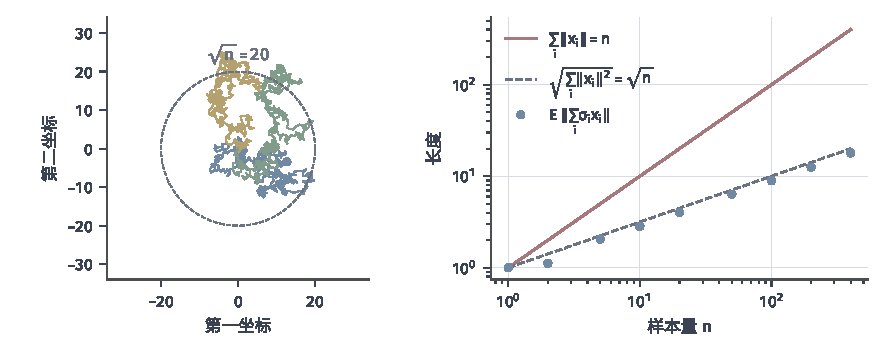
\includegraphics[width=150mm]{figures/06-foundations/02-learning-theory/matplotlib/lt7a-linear-random-walk/figure.pdf}
 \caption{线性类中随机符号和的长度。左：400个方向均匀随机的固定单位输入，三串独立随机符号下部分和$\sum_{i\leq k}\sigma_i\bm x_i$的轨迹（圆点为终点），虚线圆半径$\sqrt n=20$。右：对数坐标下$\mathbb E\|\sum_i\sigma_i\bm x_i\|_2$的蒙特卡罗估计（圆点）、均方根上界$\sqrt n$（虚线）与同向累加长度$n$（实线）。随机种子2026，数据见图源目录。}
 \label{fig:lt7a-linear-random-walk}
\end{figure*}

同一计算可以推广到预先固定的特征映射。设$\phi:X\to\mathcal H$把输入映到可分Hilbert空间$\mathcal H$，且$\|\phi(x)\|_{\mathcal H}\leq r$对几乎所有$x$成立；核$k(x,x')=\langle\phi(x),\phi(x')\rangle_{\mathcal H}$给出内积。考虑$\mathcal F_B=\{x\mapsto\langle\bm v,\phi(x)\rangle_{\mathcal H}:\|\bm v\|_{\mathcal H}\leq B\}$，即对应\term{再生核Hilbert空间}中半径$B$的球（\term{核方法}使用的正是这类函数）。

\begin{theorem}[固定特征映射的Rademacher复杂度]
\label{thm:kernel-rademacher}
在上述设定下，对任意输入样本$S_X$，
\[
 \widehat{\mathfrak R}_{S_X}(\mathcal F_B)
 \leq\frac Bn\sqrt{\sum_{i=1}^nk(x_i,x_i)}
 \leq\frac{Br}{\sqrt n}.
\]
因此下面线性预测的间隔风险界（定理~\ref{thm:linear-margin-risk}）在把$\bm w^\top\bm x$换成$\langle\bm v,\phi(x)\rangle_{\mathcal H}$后仍成立。
\end{theorem}
\begin{proof}
与式~\eqref{eq:linear-rademacher-bound}相同：Hilbert空间中的Cauchy--Schwarz不等式给出$\sup_{\|\bm v\|\leq B}\langle\bm v,\sum_i\sigma_i\phi(x_i)\rangle=B\|\sum_i\sigma_i\phi(x_i)\|_{\mathcal H}$；Jensen不等式与$\mathbb E\sigma_i\sigma_j=0$给出$\mathbb E\|\sum_i\sigma_i\phi(x_i)\|^2_{\mathcal H}=\sum_ik(x_i,x_i)$。$\mathcal H$可分，取可数稠密子集中范数不超过$B$的元素作为逼近子类，满足风险定理的可测性要求。
\end{proof}

核的作用是让有界特征范数$\sqrt{k(x,x)}\leq r$取代欧氏输入界：复杂度只通过对角元$k(x_i,x_i)$进入，特征空间可以是无限维。第~\ref{sec:ntk-rkhs-generalization}节把这一结论用于固定核近似下的网络。使用时有两点限制。第一，特征映射必须在抽样前固定；若特征或核由同一训练集选出，$\mathcal F_B$就成了依赖样本的类，不能直接当作固定类代入定理，需要把选择过程本身计入复杂度或另用独立样本。第二，公式不显含维数，并不意味着输入尺度和范数约束与维数无关：例如各坐标有界时，$r$本身可能随维数增长。

最后把线性类的复杂度与第~\ref{sec:rademacher-symmetrization-bound}节的间隔损失结合。将式~\eqref{eq:linear-rademacher-bound}经收缩引理代入定理~\ref{thm:margin-risk-bound}，就得到线性分类的完整风险界。

\begin{theorem}[线性预测的间隔风险界]
\label{thm:linear-margin-risk}
设输入几乎处处满足$\|\bm x\|_2\leq r$，标签$y\in\{-1,1\}$，$\mathcal F=\{\bm x\mapsto\bm w^\top\bm x:\|\bm w\|_2\leq B\}$，$\rho>0$在抽样前固定，得分为0时的预测事先固定。则对任意$\delta\in(0,1)$，以至少$1-\delta$的概率，所有$\|\bm w\|_2\leq B$同时满足
\begin{equation}
 R_{\mathcal P}^{01}(\operatorname{sign}f_{\bm w})
 \leq\frac1n\sum_i\ell_\rho(\bm w^\top\bm x_i,y_i)
 +\frac{2Br}{\rho\sqrt n}
 +3\sqrt{\frac{\log(2/\delta)}{2n}}.
 \label{eq:rademacher-margin-risk}
\end{equation}
\end{theorem}
\begin{proof}
$\mathcal F$以有理坐标参数为可数逼近子类。将式~\eqref{eq:linear-rademacher-bound}代入定理~\ref{thm:margin-risk-bound}即得。
\end{proof}

若经验间隔损失为零，要使右端后两项不超过$\varepsilon$，充分的样本量为$O(((Br/\rho)^2+\log(1/\delta))/\varepsilon^2)$。例如$Br/\rho=10$、$n=10^4$时，复杂度项为$2\times10/100=0.2$；要把它降到$0.02$，需要$n=10^6$。决定样本量的是范数与间隔之比$Br/\rho$，而不是输入维数；在维数很高但间隔较大的问题上，这个保证可能远好于只依据半空间VC维（维数加一）得到的保证。

使用这个界时，范数约束、输入尺度和实际间隔须一起判断。把参数整体乘以$c\in(0,1)$不改变分类结果，但所有得分间隔同比缩小，要保持经验间隔损失不变，$\rho$也须同比缩小，比值$Br/\rho$不变，界不会因此变好。等价地，可以把参数归一化，用归一化间隔$y\bm w^\top\bm x/\|\bm w\|_2$衡量拟合，此时$B=1$，界只依赖$r$与归一化间隔阈值。第~\ref{sec:linear-implicit-bias}节分析梯度下降在可分数据上的方向收敛时，正是通过这一接口把最大间隔方向连接到零一风险。这个界与二分类基本定理不矛盾：它额外利用了参数范数有界、输入有界和间隔损失三个条件，不能使VC维无限的空间在所有分布上可学习。

\subsection{输出的可重构性：样本压缩}
\label{sec:sample-compression}

Rademacher复杂度与VC维衡量的都是整个函数类：类中任何一个函数都可能被选中，所以要同时控制全部函数。换一个角度，有些训练结果不需要保存整份样本就能恢复，例如一个阈值分类器可能只需保留靠近分界的一条记录。思路是：固定少量保留记录及旁信息后，重构出的规则已经确定；若这个规则在总体上经常出错，却仍能通过其余许多观测的检验，这件事发生的概率很小。再把可能尝试的保留位置和旁信息一并计数，就能控制算法挑中“碰巧通过检验的坏规则”的概率。研究这种由少量样本重构输出的方案，称为\term{样本压缩}（sample compression）。

压缩规模因此衡量重构所需的记录与辅助描述，不是训练时访问的观测数。选择哪些记录仍可以依赖完整样本，证明必须为这种选择付出代价。本小节先由阈值例子建立压缩与重构映射，再完成可实现二分类下的风险证明，最后说明压缩规模与维度的关系，以及它为什么还不能直接当作信息量。

\subsubsection{保留样本、旁信息与重构映射}

以递增阈值$h_t(x)=\mathbb I\{x\geq t\}$为例，先看四条记录：输入$0.1,0.4$标0，$0.7,0.9$标1。只保留最小正例$(0.7,1)$，按“输入不小于$0.7$就判1”重构，得到的$h_{0.7}$判对全部四条记录。找出最小正例时检查过全部样本，只有重构时才只需一条记录。这说明了重构结构，还没有说明重构出的分类器总体风险小，后者是下一小节的任务。

同一做法适用于更多记录。图~\ref{fig:lt7a-threshold-compression}上方有8条训练记录，分数$0.08$、$0.21$、$0.35$、$0.47$的标签为0，分数$0.56$、$0.69$、$0.83$、$0.94$的标签为1。只保留分数最小的正例$(0.56,1)$，并约定以它的分数作为阈值，就重构出$h_{0.56}$，它判对全部8条记录。这里只要求重构出的分类器与训练样本一致，并不要求恢复总体上的真实阈值。这个做法对任何能被递增阈值正确分类的有限样本都适用：这样的样本中，所有负例的分数都小于最小正例，其余正例都不小于它。图下方的样本没有正例，就不保留任何记录，并约定重构出恒为0的函数。恒为0的函数不属于实数阈值空间，所以本节允许非恰当的重构。

\begin{figure}[htbp]
 \centering
 % 递增阈值 h_t(x)=I{x>=t} 的一记录压缩。
% 上行：8 条可实现样本，分数 0.08,0.21,0.35,0.47(标签0) 与 0.56,0.69,0.83,0.94(标签1)。
% 压缩：只保留最小正例 (0.56,1)；重构：t=0.56，判对全部8条。
% 下行：没有正例的样本 0.15,0.40,0.62,0.88 全为0，保留空集，重构为恒0函数。
% 横轴比例：分数 1 对应 100 mm。
\begingroup
\providecolor{FigureGreen}{HTML}{829C8B}
\providecolor{FigureGreenFill}{HTML}{E8EEE9}
\begin{tikzpicture}[figure picture,x=1mm,y=1mm]
% 第一行
\fill[FigureBlueFill] (56,24) rectangle (100,34);
\draw[FigureStroke,line width=.6pt] (0,26)--(100,26);
\foreach \x in {0,0.5,1}{\draw[FigureStroke] ({100*\x},25.2)--({100*\x},26.8); \node[figure note] at ({100*\x},22.5) {$\x$};}
\foreach \x in {0.08,0.21,0.35,0.47}{\draw[FigureRed,fill=white,line width=.8pt] ({100*\x},29) circle (1.3);}
\foreach \x in {0.69,0.83,0.94}{\fill[FigureBlue] ({100*\x},29) circle (1.3);}
\fill[FigureBlue] (56,29) circle (1.3);
\draw[FigureGreen,line width=1pt] (56,29) circle (2.6);
\draw[FigureStroke,line width=.9pt,dash pattern=on 2pt off 1pt] (56,24)--(56,36);
\node[figure note,anchor=south] at (56,36) {保留 $(0.56,1)$，重构 $t=0.56$};
\node[figure note,anchor=west] at (101,29) {$S$};
\node[figure note] at (78,31.8) {$h_t=1$};
\node[figure note] at (27,31.8) {$h_t=0$};
% 第二行
\draw[FigureStroke,line width=.6pt] (0,8)--(100,8);
\foreach \x in {0,0.5,1}{\draw[FigureStroke] ({100*\x},7.2)--({100*\x},8.8); \node[figure note] at ({100*\x},4.5) {$\x$};}
\foreach \x in {0.15,0.40,0.62,0.88}{\draw[FigureRed,fill=white,line width=.8pt] ({100*\x},11) circle (1.3);}
\node[figure note,anchor=west] at (101,11) {$S'$};
\node[figure note] at (50,15.5) {没有正例：保留空集，重构恒为 $0$ 的函数};
% 图例
\draw[FigureRed,fill=white,line width=.8pt] (4,41) circle (1.3); \node[figure note,anchor=west] at (6,41) {标签 $0$};
\fill[FigureBlue] (22,41) circle (1.3); \node[figure note,anchor=west] at (24,41) {标签 $1$};
\end{tikzpicture}
\endgroup

 \caption{递增阈值的一记录压缩。上：8条可实现记录（空心为标签0，实心为标签1），只保留最小正例$(0.56,1)$（绿圈），重构阈值$t=0.56$，浅蓝区域为预测1的范围，全部记录被判对。下：没有正例的样本保留空集，重构为恒0函数。分数为教学构造。}
 \label{fig:lt7a-threshold-compression}
\end{figure}

一个压缩方案需要事先固定两个映射。压缩映射$\kappa$读入完整样本，从中挑出要保留的记录；重构映射$\varrho$只读取这些保留的记录，输出一个分类器。有时还允许附带一段有限长的二进制串，告诉重构映射怎样使用保留的记录，这段串称为\term{旁信息}（side information）。旁信息的长度也要计入方案的规模，否则可以用很长的旁信息把整个原始样本编码进去，“只保留少量记录”就失去了意义。

\begin{definition}[一致样本压缩方案]
\label{def:sample-compression}
设$\mathcal H\subseteq\{0,1\}^X$，$k,b$为非负整数。一个$(k,b)$一致样本压缩方案由固定的确定性映射$\kappa$和$\varrho$组成。对任意有限样本$S=((x_i,y_i))_{i=1}^n$，若存在$h\in\mathcal H$使$h(x_i)=y_i$对所有$i$成立，则$\kappa(S)=(S_I,u)$满足
\[
 I\subseteq\{1,\ldots,n\},\qquad |I|\leq k,\qquad u\in\{0,1\}^b,
\]
其中$S_I$按原样本中的次序排列。重构映射仅以$(S_I,u)$为输入，输出$\varrho(S_I,u):X\to\{0,1\}$，且满足
\[
 \varrho(S_I,u)(x_i)=y_i,\qquad i=1,\ldots,n.
\]
\end{definition}

定义中有几点需要注意。同一对映射必须对每一份可实现样本都有效，$k$和$b$不能随样本量增长；重构映射也不能读取未保留的观测，或使用未计入规模的位置编号：重构器读到的全部信息都必须计入描述。阈值方案中$k=1$、$b=0$。本书把$s=k+b$称为方案的总规模，每条记录和每个比特各计一个单位；但在风险公式中，$k$与$b$的作用不同：保留的记录越多，剩下可用于检验的样本越少；旁信息越长，可能的重构结果越多。还要注意，保留哪些位置是看过完整样本后才决定的，未保留的记录也参与了这个决定，所以不能未经论证就把它们当作与输出独立的验证集。下面的定理正是为处理这一点而先固定描述、再对全部描述计数。

\subsubsection{一致压缩的风险界与学习保证}

与第~\ref{sec:binary-finite-class}节一样，与样本一致本身不能保证风险低。压缩方案的作用在于限制可能的重构结果：每个输出都由一个描述，即保留哪些位置以及取哪段旁信息，唯一确定。从$n$个样本中保留$j$个位置有$\binom nj$种选法，旁信息至多有$2^b$种，描述总数至多为$2^b\sum_{j=0}^k\binom nj$。固定一种描述后，高风险的重构分类器要判对全部未保留的观测，概率很小；再对全部描述把失败概率相加。

\begin{theorem}[一致样本压缩的期望风险上界]
\label{thm:sample-compression-bound}
设$(X,\mathcal X)$为可测空间，$Y=\{0,1\}$取离散$\sigma$代数，$\mathcal H\subseteq Y^X$是由可测分类器组成的非空集合，$k,b$为非负整数。设可测确定性映射$\kappa,\varrho$构成定义~\ref{def:sample-compression}中的$(k,b)$一致压缩方案，并假定对$\varrho$可能输出的每个$h$，函数$(x,y)\mapsto\mathbb I\{h(x)\neq y\}$均可测。令$\mathcal P$为$X\times Y$上的联合分布，存在$h^\star\in\mathcal H$满足$\mathbb P_{(x,y)\sim\mathcal P}\{h^\star(x)\neq y\}=0$。若$n>k$且$S\sim\mathcal P^n$，则对任意$\delta\in(0,1)$，以至少$1-\delta$的概率，重构分类器$h_S=\varrho(\kappa(S))$的零一损失期望风险满足
\begin{equation}
 R_{\mathcal P}(h_S)
 \leq\frac{b\log2+\log\!\left(\sum_{j=0}^k\binom nj\right)+\log(1/\delta)}{n-k}.
 \label{eq:compression-generalization}
\end{equation}
概率仅来自独立同分布样本$S\sim\mathcal P^n$。
\end{theorem}

\begin{proof}
先固定一种描述$(I,u)$，其中$|I|=j\leq k$，而不条件于压缩映射选中它。给定$S_I$，重构$h_{I,u}=\varrho(S_I,u)$已确定，余下$n-j$个观测仍独立服从$\mathcal P$。若其风险超过$\varepsilon$，这些观测全被分对的条件概率至多为
\[
 (1-\varepsilon)^{n-j}\leq e^{-(n-j)\varepsilon}\leq e^{-(n-k)\varepsilon}.
\]
再对$S_I$平均，可知该固定描述同时导致高风险和全样本一致的概率至多$e^{-(n-k)\varepsilon}$。可实现性保证样本以概率1可由$h^\star$正确分类，最终输出总由某个$(I,u)$重构并与全样本一致；输出风险超过$\varepsilon$时，至少一种描述满足前述失败事件。对全部描述作并集界得到
\[
 \mathbb P\{R_{\mathcal P}(h_S)>\varepsilon\}
 \leq 2^b\left(\sum_{j=0}^k\binom nj\right)e^{-(n-k)\varepsilon}.
\]
令右侧至多为$\delta$，取对数并整理即得式~\eqref{eq:compression-generalization}。若所列上界不小于1，零一风险本身至多为1已保证结论。
\end{proof}

证明中固定的是事先枚举的候选描述，不是“压缩映射最终选中的那一个”。若条件于选中事件，未保留观测就参与过这次选择，独立性不再自动成立；先对每个固定描述计算通过概率、再对全部描述求并，才覆盖了数据依赖的选择。式~\eqref{eq:compression-generalization}的两项由此而来：可选描述越多，选择代价越大，描述个数的对数出现在分子上；剩余用于检验的观测越多，坏规则全部蒙对的概率越小，未保留观测的个数（至少$n-k$）出现在分母上。两项条件各司其职：训练一致性保证实际输出通过了全样本检验，可实现性与统一的压缩方案保证这样的输出在所讨论的样本上存在。$\log$是自然对数，$b$个比特贡献$b\log2$。阈值方案取$k=1$、$b=0$，组合数之和为$n+1$，得到
\[
 R_{\mathcal P}(h_S)\leq\frac{\log(n+1)+\log(1/\delta)}{n-1}.
\]
例如$n=100$、$\delta=0.05$时，分子为$\log101+\log20\approx4.615+2.996=7.61$，右端约为$7.61/99\approx0.077$，即以至少95\%的概率，重构出的阈值错误率不超过7.7\%。这是一般压缩界给出的充分保证，不能据此断言阈值类的最优样本量必定含有$\log n$因子。

\begin{theorem}[有界样本压缩推出PAC可学习]
\label{thm:compression-pac-learning}
在定理~\ref{thm:sample-compression-bound}的可测性条件下，设$k,b$为固定非负整数，$(\kappa,\varrho)$是$\mathcal H$的$(k,b)$一致压缩方案。则确定性学习算法$A(S)=\varrho(\kappa(S))$使$\mathcal H$在允许非恰当输出的意义下可实现PAC可学习。具体地，对任意$\varepsilon,\delta\in(0,1)$、任意$\mathcal H$可实现分布$\mathcal P$和$S\sim\mathcal P^n$，只要$n>k$且
\[
 b\log2+\log\!\left(\sum_{j=0}^k\binom nj\right)+\log(1/\delta)\leq(n-k)\varepsilon,
\]
就有$\mathbb P_{S\sim\mathcal P^n}\{R_{\mathcal P}(A(S))\leq\varepsilon\}\geq1-\delta$，且这一样本量条件不依赖具体的可实现分布。
\end{theorem}

\begin{proof}
$k=0$时组合数和为1；固定$k\geq1$时，$\sum_{j=0}^k\binom nj\leq(k+1)n^k$。分子至多按$\log n$增长，分母按$n$增长，故任意给定$\varepsilon,\delta$都存在有限门槛，使此后所有$n$满足条件。将这些$n$代入前一定理，即得到分布无关的风险保证。
\end{proof}

前一个定理对给定样本量给出输出风险的高概率上界，后一个说明同一个算法在所有可实现分布上都能达到任意精度；有限样本上界逐个$n$成立，统一可学习性则来自门槛不依赖分布。二者都依赖训练一致性：标签有噪声或重构不一致时，一致的重构可能不存在，原定理不能直接使用。一般损失或不可知情形需要另行证明，例如在第~\ref{sec:ds-compression-proof}节中，还要证明重构候选里存在经验风险足够低者，并计入读取样本造成的偏差。此外，压缩映射和重构映射的存在并不说明怎样计算它们，也不说明需要多少计算时间。
\subsubsection{压缩规模、维度与信息量}

VC维限制假设空间在有限输入上能自由实现的标注，压缩规模限制一致输出所需的描述数，二者都衡量复杂程度。一个方向可以由已有结果推出：统一有界的压缩方案推出可实现PAC，再由二分类学习基本定理推出VC维有限。下面的定理不经过学习理论，直接用计数说明这一点。

\begin{theorem}[压缩参数对打散的限制]
\label{thm:compression-shattering-count}
设$X$为非空集合，$\mathcal H\subseteq\{0,1\}^X$非空，$k,b$为非负整数。假定存在$\mathcal H$的$(k,b)$一致压缩方案$(\kappa,\varrho)$。若$\mathcal H$能打散$m\geq1$个不同输入，则
\[
 2^m\leq 2^b\sum_{j=0}^{\min\{k,m\}}\binom mj2^j.
\]
特别地，固定有限的$k,b$意味着$\operatorname{VC}(\mathcal H)<\infty$。
\end{theorem}

\begin{proof}
把被打散的$m$个输入按固定次序排列，全部$2^m$种标签都对应可实现样本。大小$j$的保留集有$\binom mj$种，它的标签有$2^j$种，旁信息另有$2^b$种，合计为右侧的描述数。两份不同完整标签若压缩成同一描述，确定性的重构就须在某个输入给出两种标签，矛盾。故描述数至少$2^m$。固定$k,b$后，描述数随$m$至多多项式增长，无法始终覆盖指数增长的$2^m$，所以VC维有限。
\end{proof}

例如阈值方案$k=1$、$b=0$时，右侧为$1+2m$。$m=1$时$2\leq3$成立，$m=2$时$4\leq5$成立，$m=3$时$8>7$，故该方案对应的类不能打散3个点；递增阈值实际的VC维为1，计数界只给出上限2，并不精确。

反方向也成立：VC维有限时，存在规模与样本量无关的压缩方案，这是组合意义上的存在性结论。按$s=k+b$计，Moran与Yehudayoff为VC维为$d$的二分类空间构造了规模$s=2^{O(d)}$的方案\scite{moran2016compression}。要把这个方案代入风险定理得到PAC结论，还需验证它的压缩映射、重构映射和输出损失满足前面的可测条件；组合构造本身不提供这一步，也没有确定最小的压缩规模。\term{样本压缩猜想}（sample compression conjecture）断言规模可以达到$s=O(d)$，Attias等人2025年的工作仍把一般情形列为未解决问题\scite{attias2025compression}。比较不同方案的规模时，记录数和旁信息长度必须一并计算。组合方案的存在、方案的可测实现以及计算效率是三个不同的问题。

Rademacher分析与压缩分析控制的对象不同。前者控制损失类中所有函数拟合随机符号的能力；后者固定重构映射，并在一份给定的完整训练样本上枚举保留位置和有限旁信息，从而得到有限组候选输出。改变完整样本后，重构输出仍可能有无穷多种，因此有限的是每份样本内的描述组合，不是重构映射在所有可能样本上的像集。压缩分析计入这种描述选择，而不要求以同样精度评价整个假设空间，所以不能把压缩规模$s$直接代入Rademacher复杂度的公式。两者的适用条件也不同：Rademacher界允许经验风险不为零；本节的压缩界要求训练一致，在$k,b$固定时得到约$\log n/n$的速率。条件不同，不能只按收敛速率比较优劣。此外，某一份样本碰巧能被压缩并不能推出PAC，必须存在同一个方案，对所有可实现样本都保持统一的规模。

直观上，压缩方案限制了输出“能说出多少关于样本的事”：给定完整样本后，输出只是有限个描述之一。但记录条数不等于比特数。设观测取自$[0,1]$上的连续分布，方案原样保留第一条观测，输出就是这个数，$k=1$、$b=0$；输出却精确揭示了一个连续取值的观测，下一小节将看到，这时输出与样本的普通互信息为无穷。所以小压缩规模不能直接当作小的普通互信息。本节约束的只是重构结构；第~\ref{sec:conditional-information}节定义条件互信息以后，再证明在给定候选观测池时，有限的记录选择怎样限制输出透露的信息。

\subsubsection{多分类学习保证的压缩证明路线（选读）}
\label{sec:ds-compression-proof}

第~\ref{sec:ds-dimension}节已经独立陈述了有限DS维的学习保证（定理~\ref{thm:finite-ds-learnability}），并说明它所依赖的学习器构造来自外部文献。本小节补充这条保证经样本压缩的详细推导，供希望核对风险计算的读者阅读；理解DS维的定义、必要性和刻画结论不需要先读本小节。

DS维有限时不能借助一致收敛，因为第~\ref{sec:general-multiclass-dimensions}节的集合标签例子表明一致收敛可能不成立，必须直接构造学习算法。Brukhim等人构造的正是一种样本压缩，做法分两步：先由少量样本重构一个标签列表，为每个输入给出少数几个候选标签；再在列表范围内重构单一标签\scite{brukhim2022multiclass}。\term{列表预测}（list prediction）不直接给出一个类别，而是在每个输入$x$上返回一个有限的候选标签集合$\mu(x)\subseteq Y$，把无限多个可能的标签缩小到少数几个。说列表预测覆盖样本，是指每个样本的真实标签都在该样本输入对应的列表中。下面先陈述借用的构造，本书不证明它。

\begin{lemma}[有限DS维的压缩构造]
\label{lem:finite-ds-compression}
设$X,Y$为非空集合，$\mathcal H\subseteq Y^X$非空，且$d=d_{DS}(\mathcal H)<\infty$。存在通用常数$C>0$，使得对每个整数$n\geq1$，以及每份大小$q\leq n$、可由某个$h\in\mathcal H$正确分类的带标签样本$S=((x_i,y_i))_{i=1}^q$，均存在如下压缩表示：从$S$中选取一个允许重复、保留次序的带标签序列，长度至多
\[
 r_n=\min\!\left\{n,\left\lceil C(d+1)^{3/2}\log^2\!\bigl(2n(d+1)\bigr)\right\rceil\right\},
\]
并记录原样本大小$q$。对每个$q\leq n$，存在不依赖具体样本的固定重构映射，仅根据$q$和该压缩序列输出分类器$\varrho_q:X\to Y$，且$\varrho_q(x_i)=y_i$对$i=1,\ldots,q$均成立。重构分类器不要求属于$\mathcal H$。
\end{lemma}

引理是原文定理36的表述，常数和对数因子作了放宽。原文先用有限DS维重构一个覆盖原样本的列表（引理39），再用有限Natarajan维在列表范围内重构一致的单标签分类器（引理40）；把两段压缩序列拼接起来即可依次完成重构，而$d_N\leq d$保证第二步的规模也受$d$控制。上界超过$n$时，直接保存全部样本即可。列表部分借用了原文的超图定向技术，本书只说明这个构造如何进入压缩与风险分析。描述由三部分组成：原样本大小$q$、压缩序列的长度，以及允许重复的有序索引；压缩长度只随$n$按$\log^2n$增长、随DS维按$(d+1)^{3/2}$增长，与标签总数无关，这正是它能处理无限标签的原因。
接下来统计可能的描述有多少，再沿用定理~\ref{thm:sample-compression-bound}的思路同时控制所有重构结果。计数只依赖序列长度，与标签总数无关。与二分类一致压缩相比有两处新增步骤：描述允许重复索引，固定描述后要条件于它实际读取的不同观测；不可知情形还要证明重构候选中存在经验风险不高于类内参照者，并计入读取样本造成的偏差。

\begin{theorem}[有限DS维的期望风险保证]
\label{thm:finite-ds-learning-rates}
设$(X,\mathcal X)$为可测空间，$Y$为离散标签空间，$\mathcal H\subseteq Y^X$是由可测分类器组成的非空集合，$d=d_{DS}(\mathcal H)<\infty$，并采用零一损失。取引理~\ref{lem:finite-ds-compression}中的常数$C$与长度$r_n$，固定满足$r=r_n<n$的$n$。假定每个候选分类器的零一损失函数，以及所用压缩、重构和有限候选选择映射均可测。预先固定一个$h_0\in\mathcal H$和全部压缩描述的顺序；对每份$S=((x_i,y_i))_{i=1}^n$，枚举由原样本大小、至多$r$个允许重复且保留次序的样本索引组成的描述，用固定重构映射产生候选，无效描述统一返回$h_0$。令$A^{\mathrm{real}}$选择顺序最先且与$S$一致的候选，若不存在则返回$h_0$；令$A^{\mathrm{agn}}$选择顺序最先且零一经验风险最小的候选。记
\[
 B_n(\delta)=\log\frac{2(n+1)(r+1)n^r}{\delta}.
\]
这两个确定性算法允许输出$\mathcal H$之外的可测分类器。对任意$\delta\in(0,1)$，以下保证成立：
\begin{enumerate}
\item 对任意$X\times Y$上的联合分布$\mathcal P$，若存在$h^\star\in\mathcal H$满足$R_{\mathcal P}(h^\star)=0$，则对$S\sim\mathcal P^n$，以至少$1-\delta$的概率，
 \[
 R_{\mathcal P}(A^{\mathrm{real}}(S))\leq\frac{B_n(\delta)}{n-r}.
 \]
\item 对任意$X\times Y$上的联合分布$\mathcal P$和$S\sim\mathcal P^n$，以至少$1-\delta$的概率，
 \[
 R_{\mathcal P}(A^{\mathrm{agn}}(S))
 \leq\inf_{h\in\mathcal H}R_{\mathcal P}(h)+\frac rn
 +\sqrt{\frac{B_n(\delta)}{2(n-r)}}+\sqrt{\frac{\log(2/\delta)}{2n}}.
 \]
\end{enumerate}
其中$R_{\mathcal P}$为零一损失期望风险，两项概率都只来自独立同分布样本。
\end{theorem}

\begin{proof}[证明（使用引理~\ref{lem:finite-ds-compression}）]
候选分类器虽然依赖样本，但每个候选只由至多$r$条样本决定，其余样本对它而言仍是独立的检验数据；再对所有可能的描述作并集界。

先数描述。长度为$j$、允许重复的有序索引序列有$n^j$种，$j=0,\ldots,r$合计至多$(r+1)n^r$种；再计$n+1$种原样本大小，描述总数至多$M=(n+1)(r+1)n^r$。这些索引在观察训练样本前确定，未预先列举无限标签。抽取训练样本前固定$h_0$和描述顺序，重构补为总映射，每份样本便有至多$M$个有序候选；可实现算法取首个全一致者，压缩引理保证它存在；不可知算法取首个经验最小者。题设的可测映射使这两种有限选择也可测。

可实现情形。固定一个索引描述，设它实际读取$j\leq r$个不同观测。给定这些观测的值后，候选分类器已经确定，而其余$n-j$个观测与它们独立，仍是独立同分布的。风险大于$u$的候选将其余$n-j$个观测全部正确分类的概率至多为$(1-u)^{n-j}\leq e^{-(n-r)u}$。对$M$种描述作并集界，就覆盖首个全一致输出；取$u=B_n(\delta)/(n-r)$，失败概率至多$Me^{-B_n(\delta)}=\delta/2\leq\delta$，得到可实现界；$u\geq1$时用风险不超过1的平凡保证。

不可知情形分三步。第一步，对固定描述，以$\hat R_{\mathrm{rest}}$记未读取观测上的损失平均。条件独立性与单侧Hoeffding不等式，再跨$M$个描述求和，使下式以至少$1-\delta/2$的概率对全部候选同时成立：
\[
 R_{\mathcal P}(h)\leq\hat R_{\mathrm{rest}}(h)+\sqrt{\frac{\log(2M/\delta)}{2(n-r)}}.
\]
这里$\log(2M/\delta)=B_n(\delta)$。第二步，把$\hat R_{\mathrm{rest}}$换回全样本的经验风险。记已读观测上的平均损失为$\hat R_{\mathrm{read}}$，则$\hat R_S=\frac{n-j}n\hat R_{\mathrm{rest}}+\frac jn\hat R_{\mathrm{read}}$，于是
\[
 \hat R_{\mathrm{rest}}-\hat R_S=\frac jn\bigl(\hat R_{\mathrm{rest}}-\hat R_{\mathrm{read}}\bigr)\leq\frac jn\leq\frac rn,
\]
这里用到零一损失的平均值在$[0,1]$中；代价是多出一项$r/n$。第三步，说明经验最小的候选不比类内的好分类器差。任意预先固定$g\in\mathcal H$，把由$g$正确分类的观测组成可实现子样本，压缩引理提供在这些观测上全部分类正确的重构者，它出现在候选中，经验风险至多$\hat R_S(g)$；子样本为空时，$\hat R_S(g)=1$，任意候选都不更大。经验最小重构于是满足$\hat R_S(A^{\mathrm{agn}}(S))\leq\hat R_S(g)$。对固定$g$再用Hoeffding不等式，以至少$1-\delta/2$的概率$\hat R_S(g)\leq R_{\mathcal P}(g)+\sqrt{\log(2/\delta)/(2n)}$。合并两个半失败预算即得到相对该$g$的风险界。任取$\tau>0$，在抽样前选风险距类内下确界不足$\tau$的$g$，得到超过所列上界加$\tau$的概率至多$\delta$；令$\tau\downarrow0$，由事件单调收敛得到第二结论，无需所有参照同时估准。
\end{proof}

两个界的主项都由$B_n(\delta)\approx r\log n+\log(1/\delta)$决定：$r\log n$是为“看过样本后才选择保留哪些记录”付出的代价，$\log(1/\delta)$来自失败概率。固定$d$时$r_n=O(\log^2n)$，所以$r_n/n\to0$，两个风险界分别趋于零和$\mathcal H$中的最低风险；这正是压缩规模与样本量之比趋零的用途。略去$n$和$d$的对数因子，可实现情形的风险为$\widetilde O((d^{3/2}+\log(1/\delta))/n)$，不可知情形的超额风险为$\widetilde O(\sqrt{(d^{3/2}+\log(1/\delta))/n})$。这些都是统计存在性保证，并不说明压缩和搜索步骤可以计算，更不说明能在多项式时间内完成；所需的可测性也是题设，不由组合维数有限自动得到。
\subsection{输出的信息依赖：信息论界}
\label{sec:information-stability}

压缩给出了限制输出的一种具体做法：输出只能是有限个描述之一。信息方法进一步追问：即使找不到可见的压缩子样本，能否直接衡量训练输出对这份样本的依赖？先设想一个参照过程：保持输出的分布不变，却让输出与评价样本独立配对。这个过程中没有“看过考题再评分”的依赖，平均经验损失与平均总体风险相同；实际训练把两者联系起来，信息量用来控制这种联系可能造成的评价偏差。恒定输出不含任何样本信息，逐字保存训练样本则保留全部信息。

本小节据此区分三个问题。普通互信息衡量输出与整份样本的统计依赖；条件互信息衡量已知候选观测后，输出透露了哪些训练选择；PAC--Bayes控制从训练前的决策分布调整到训练后决策分布的代价。下面先建立共同的换测度工具和互信息界，再依次处理条件互信息与PAC--Bayes，最后说明互信息与PAC--Bayes两种代价怎样联系。信息量小首先约束评价偏差，不能代替模型本身拟合得好。

\subsubsection{换测度与互信息泛化界}

回到第~\ref{sec:generalization-tools}节开头的两个常值分类器。按多数标签选择时，选中$h_0$与$h_1$的概率各为$1/2$。保持训练样本的分布和这一输出频率不变，但改成独立地抽取输出与样本：先抛硬币决定输出$h_0$或$h_1$，再另抽三条标签评价它。这时不再优先选中这份样本上成绩较好的分类器，训练错误率的平均回到$1/2$，与总体错误率相同。一般地，设想一个参照过程：分别从样本和输出的边缘分布中独立抽取，二者各自的分布不变，只消除了依赖。在参照过程中，输出与样本独立，经验风险就是期望风险的无偏估计。真实训练与参照过程的差别，用联合分布$P_{S,W}$与乘积分布$P_S\otimes P_W$之间的\term{相对熵}（relative entropy）衡量。对离散分布，$D_{\mathrm{KL}}(P\|Q)=\sum_xP(x)\log(P(x)/Q(x))$，即按$P$平均的对数概率比；$P$把概率放在$Q$认为不太可能的地方越多，它就越大。相对熵非负，当且仅当两分布相同时为零，但一般不对称，不能当作距离使用（可参考\BookChapterRef{chap:information-theory-and-statistical-geometry}{卷4《数学准备：流形、概率分布与统计推断》的“概率分布的分析与优化”章}）。样本与输出的\term{互信息}（mutual information）就是
\[
 I(W;S)=D_{\mathrm{KL}}(P_{S,W}\|P_S\otimes P_W).
\]
它衡量输出与样本之间的统计依赖，不是参数个数，也不是模型文件的大小：一个只有一个参数的模型，若把训练样本的精确值写进这个参数，互信息可以很大。

图~\ref{fig:lt7a-joint-product-information}给出一个可以手算的例子。观测$z_1$等概率取0或1，算法以概率$0.9$输出$W=z_1$、以概率$0.1$输出$1-z_1$。联合分布在对角格各放$0.45$，非对角格各放$0.05$；乘积分布每格$0.25$。于是
\[
 I(W;z_1)=2\times0.45\log\frac{0.45}{0.25}+2\times0.05\log\frac{0.05}{0.25}\approx0.529-0.161=0.368
\]
（自然对数），也等于$\log2-h(0.1)$，其中$h$为二元熵。若算法精确输出$W=z_1$，互信息为$\log2\approx0.693$，一个比特；若算法逐字输出整份二值样本，互信息为$n\log2$，随样本量线性增长。信息方法用这种增长速度衡量记忆程度。图右侧是连续情形：$z_1$取自$[0,1]$上的均匀分布而$W=z_1$，联合分布全部落在对角线上，乘积分布给这条线的概率为零，相对熵为无穷。

\begin{figure*}[htbp]
 \centering
 % 换测度前后的联合分布与乘积分布。
% 设定：z1 等概率取 0、1；算法以概率 1-q 输出 W=z1、以概率 q 输出 1-z1，q=0.1。
% 联合分布 P(z1,W)：对角 0.45，非对角 0.05；乘积分布 P(z1)P(W)：每格 0.25。
% 互信息 I(W;z1)=sum P log(P/Q)=2*0.45*log(1.8)+2*0.05*log(0.2)=log2-h(0.1)≈0.368 nat。
% 右图：连续情形 n=1，z1~U[0,1]，精确输出样本均值 W=z1。
% 联合分布全部质量在对角线 w=z1 上（面积为零），乘积分布为正方形上的均匀分布，
% 后者给对角线的概率为 0，故 KL 与互信息为无穷。此面板只作示意。
\begingroup
\providecolor{FigureGreen}{HTML}{829C8B}
\providecolor{FigureGreenFill}{HTML}{E8EEE9}
\begin{tikzpicture}[figure picture,x=1mm,y=1mm]
\def\cell#1#2#3#4{% x y value fill-shade
 \fill[FigureBlue!#4!white] (#1,#2) rectangle ({#1+12},{#2+12});
 \draw[FigureStroke,line width=.5pt] (#1,#2) rectangle ({#1+12},{#2+12});
 \node at ({#1+6},{#2+6}) {$#3$};}
% 联合分布
\node[figure heading] at (24,38) {联合分布 $P_{z_1,W}$};
\cell{12}{12}{0.45}{55}\cell{24}{12}{0.05}{6}
\cell{12}{0}{0.05}{6}\cell{24}{0}{0.45}{55}
% 坐标: 上行 z1=0，下行 z1=1；左列 W=0，右列 W=1
\node[figure note] at (18,26.5) {$W=0$};\node[figure note] at (30,26.5) {$W=1$};
\node[figure note,anchor=east] at (11,18) {$z_1=0$};\node[figure note,anchor=east] at (11,6) {$z_1=1$};
% 乘积分布
\node[figure heading] at (68,38) {乘积分布 $P_{z_1}\otimes P_W$};
\cell{56}{12}{0.25}{28}\cell{68}{12}{0.25}{28}
\cell{56}{0}{0.25}{28}\cell{68}{0}{0.25}{28}
\node[figure note] at (62,26.5) {$W=0$};\node[figure note] at (74,26.5) {$W=1$};
\draw[FigureStroke,line width=.8pt,-{Stealth[length=1.6mm]}] (40,12)--(52,12);
\node[figure note] at (46,15.5) {消除依赖};
\node[figure note] at (46,-5.5) {$I(W;z_1)=\mathrm{KL}(P_{z_1,W}\,\|\,P_{z_1}\otimes P_W)\approx0.368$};
% 连续情形示意
\node[figure heading] at (113,38) {连续输出 $W=z_1$};
\fill[FigureBlueFill] (101,0) rectangle (125,24);
\draw[FigureStroke,line width=.5pt] (101,0) rectangle (125,24);
\draw[FigureBlue,line width=1.6pt] (101,0)--(125,24);
\node[figure note] at (113,26.5) {横轴 $z_1$，纵轴 $W$};
\node[figure note] at (113,-5.5) {浅底：乘积分布；对角线：联合分布};
\end{tikzpicture}
\endgroup

 \caption{换测度前后的联合分布与乘积分布。左、中：$z_1$等概率取0、1，算法以概率0.9输出$W=z_1$，联合分布与消除依赖后的乘积分布逐格比较，相对熵即互信息$\log2-h(0.1)\approx0.368$。右：连续观测且$W=z_1$时，联合分布集中在对角线（面积为零）上，乘积分布铺满正方形，相对熵无穷。数值为教学构造。}
 \label{fig:lt7a-joint-product-information}
\end{figure*}

把这种依赖转化为评价偏差，需要下面的换测度不等式：在$P$下计算的期望，至多比参照分布$Q$下“能取得的值”多出相对熵这一代价，而$Q$下的值由指数矩控制。

\begin{lemma}[换测度不等式]
\label{lem:change-of-measure}
设$P,Q$为同一可测空间上的概率分布，$P\ll Q$且$D_{\mathrm{KL}}(P\|Q)<\infty$。对任意下方有界的可测函数$g$，若$\mathbb E_Qe^g<\infty$，则$\mathbb E_Pg$有定义且
\begin{equation}
 \mathbb E_Pg\leq D_{\mathrm{KL}}(P\|Q)+\log\mathbb E_Qe^g.
 \label{eq:change-of-measure-general}
\end{equation}
\end{lemma}
\begin{proof}
先设$g$有界。定义倾斜分布$\mathrm dG=e^g\,\mathrm dQ/\mathbb E_Qe^g$，它与$Q$相互绝对连续。于是
\[
\begin{aligned}
 D_{\mathrm{KL}}(P\|Q)&=\mathbb E_P\log\frac{\mathrm dP}{\mathrm dQ}
 =\mathbb E_P\log\frac{\mathrm dP}{\mathrm dG}+\mathbb E_Pg-\log\mathbb E_Qe^g\\
 &=D_{\mathrm{KL}}(P\|G)+\mathbb E_Pg-\log\mathbb E_Qe^g.
\end{aligned}
\]
由$D_{\mathrm{KL}}(P\|G)\geq0$即得不等式。对下方有界的一般$g$，令$g_M=\min\{g,M\}$，对$g_M$应用已证结论；$M\to\infty$时左侧由单调收敛趋于$\mathbb E_Pg$，右侧的$\mathbb E_Qe^{g_M}$不超过$\mathbb E_Qe^g$。
\end{proof}

这一不等式是Donsker--Varadhan变分表示的一侧；当$g=\log(\mathrm dP/\mathrm dQ)$时取等号。它是本小节所有信息界共享的工具：只需为$Q$下的指数矩找到上界，再用相对熵支付从$Q$换到$P$的代价。

\begin{definition}[互信息稳定性]
\label{def:mutual-information-stability}
设$S\sim\mathcal P^n$，$W=A_n(S,U)$，$U$独立于$S$。若存在不依赖$\mathcal P$的非负序列$\iota_n$，使$I(W;S)\leq\iota_n$对所有允许分布成立，且$\iota_n/n\to0$，则称算法序列具有在允许分布族上统一的互信息稳定性。
\end{definition}

要求的是总互信息除以样本量趋于零，而不是总互信息本身趋于零。例如互信息按$\log n$增长仍满足条件。Russo与Zou用信息量控制自适应分析中的选择偏差\scite{russo2016bias}，Xu与Raginsky把样本与输出之间的互信息用于期望泛化差\scite{xu2017information}。

\begin{theorem}[互信息与期望风险]
\label{thm:mutual-information-risk}
设$(Z,\mathcal Z)$与$(\mathcal W,\mathcal B_{\mathcal W})$为可测空间，$\ell:\mathcal W\times Z\to[0,1]$可测，$\mathcal P$为$Z$上的概率分布。令$S\sim\mathcal P^n$，内部随机数$U$独立于$S$，可测算法输出$W=A(S,U)$。则
\begin{equation}
 \left|\mathbb E[R_{\mathcal P}(W)-\hat R_S(W)]\right|\leq\sqrt{\frac{I(W;S)}{2n}}.
 \label{eq:mutual-information-generalization}
\end{equation}
\end{theorem}
\begin{proof}
若$I(W;S)=\infty$，结论平凡。以下设互信息有限，此时$P=P_{S,W}\ll Q=P_S\otimes P_W$。记$g(S,W)=R_{\mathcal P}(W)-\hat R_S(W)$。在$Q$下，给定$W$后样本仍然独立同分布，$g$是$n$个独立、均值为零的量$R_{\mathcal P}(W)-\ell(W,z_i)$的平均，每个量的取值范围长度不超过1；Hoeffding引理给出$\log\mathbb E_Qe^{\lambda g}\leq\lambda^2/(8n)$对一切$\lambda\in\mathbb R$成立。$\lambda g$有界，对任意$\lambda>0$由引理~\ref{lem:change-of-measure}，
\begin{equation}
 \lambda\mathbb E_Pg\leq D_{\mathrm{KL}}(P\|Q)+\log\mathbb E_Qe^{\lambda g}.
 \label{eq:information-change-measure}
\end{equation}
因此$\mathbb E_Pg\leq I(W;S)/\lambda+\lambda/(8n)$。右侧第一项随$\lambda$减小、第二项随$\lambda$增大，取$\lambda=\sqrt{8nI(W;S)}$使两项相等，得到$\mathbb E_Pg\leq\sqrt{I(W;S)/(2n)}$；互信息为零时令$\lambda\to\infty$。对$-g$作相同推导即得绝对值形式。
\end{proof}

证明的三步正对应“独立时容易评价—实际训练引入依赖—为这种依赖支付信息代价”：在乘积分布下，输出与样本独立，固定输出后用Hoeffding引理控制指数矩；实际联合分布与乘积分布不同，换测度不等式把参照过程中的控制转回实际分布；转换的代价是两者之间的相对熵，也就是互信息。用硬币例子核对：多数选择$W$由$S$确定且两种取值各占一半，$I(W;S)=H(W)=\log2\approx0.693$，右侧为$\sqrt{0.693/6}\approx0.340$，确实不小于实际的平均评价偏差$1/2-1/4=1/4$。

这个界只约束期望泛化差，即平均评价偏差，没有给出单次训练的高概率界。若输出只能取预先给定的$K$个决策，互信息不超过输出熵，而输出熵不超过$\log K$，所以可取$\iota_n=\log K$；例如$K=1024$、$n=1000$时右侧为$\sqrt{\log1024/2000}\approx0.059$。恒定输出同样满足$I(W;S)=0$，它只有在经验优化误差也很小时才能接近最优风险。

\begin{theorem}[互信息稳定性与可学习性]
\label{thm:mutual-information-learning}
在定理~\ref{thm:mutual-information-risk}的设定下，设$\mathcal W$非空，风险下确界为有限实数且可测。若存在不依赖$\mathcal P$的非负数$\iota_n,\rho_n$，使所有允许分布满足$I(W;S)\leq\iota_n$与$\mathbb E[\hat R_S(W)-\inf_w\hat R_S(w)]\leq\rho_n$，则
\[
 \mathbb E R_{\mathcal P}(W)-\inf_{w\in\mathcal W}R_{\mathcal P}(w)\leq\sqrt{\frac{\iota_n}{2n}}+\rho_n.
\]
若$\iota_n/n\to0$且$\rho_n\to0$，算法相对于允许族统一地PAC学习此问题。
\end{theorem}
\begin{proof}
定理~\ref{thm:mutual-information-risk}给出$g_n=\sqrt{\iota_n/(2n)}$，代入定理~\ref{thm:generalization-optimization-learning}。
\end{proof}

整份样本与输出的互信息把所有依赖合并成一个数。若希望分别衡量各观测对输出的贡献，可以逐项比较单个观测与输出\scite{bu2020information}。

\begin{theorem}[逐观测互信息的期望风险界]
\label{thm:individual-information-risk}
在定理~\ref{thm:mutual-information-risk}的设定下，记$I(W;z_i)=D_{\mathrm{KL}}(P_{W,z_i}\|P_W\otimes\mathcal P)$，则
\[
 \left|\mathbb E[R_{\mathcal P}(W)-\hat R_S(W)]\right|\leq\frac1n\sum_{i=1}^n\sqrt{\frac{I(W;z_i)}2}.
\]
\end{theorem}
\begin{proof}
对每个$i$，比较$(W,z_i)$的联合分布与$P_W\otimes\mathcal P$。在乘积分布下，$R_{\mathcal P}(W)-\ell(W,z_i)$的条件均值为零、取值范围长度不超过1。沿用前一证明中样本量为1的指数矩论证，得到$|\mathbb E[R_{\mathcal P}(W)-\ell(W,z_i)]|\leq\sqrt{I(W;z_i)/2}$。对$n$项平均，再用三角不等式即可。
\end{proof}

右侧的逐观测信息代价与经验优化误差相加，同样给出平均超额风险界。普通互信息对连续输出可能取无穷，即使算法本身能很好地泛化。设观测取值于$[0,1]$，均值为$\mu$、方差为$\sigma^2$，算法精确输出样本均值$\bar z$，用平方损失评价。对独立观测有$R_{\mathcal P}(\bar z)=\sigma^2+(\bar z-\mu)^2$，所以$\mathbb E_SR_{\mathcal P}(\bar z)=\sigma^2+\sigma^2/n$；由恒等式$\sum_i(z_i-\bar z)^2=\sum_i(z_i-\mu)^2-n(\bar z-\mu)^2$，$\mathbb E_S\hat R_S(\bar z)=\sigma^2-\sigma^2/n$。期望泛化差因此为$2\sigma^2/n$，趋于零；$[0,1]$上的均匀分布有$\sigma^2=1/12$，差为$1/(6n)$。但$W=\bar z$由$S$完全确定，联合分布集中在关系$W=\bar z$上，乘积分布给这个关系的概率为零，所以$I(W;S)=\infty$，与图~\ref{fig:lt7a-joint-product-information}右侧的情形相同。算法可以泛化，普通互信息界却给不出有限数值；因此不能把小互信息视为所有学习算法都必需的性质。这一局限来自所衡量的对象：普通互信息记录了观测数值本身。下一小节改变要衡量的信息对象。
\subsubsection{条件互信息与选择信息}
\label{sec:conditional-information}

为避免连续观测的无限精度进入信息量，Steinke与Zakynthinou改为衡量“选择信息”\scite{steinke2020conditional}。先独立抽取$n$对观测，每对中随机选一个进入训练；在已知全部$2n$个备选观测的条件下，只衡量输出额外透露了“每对选了哪一个”。每个位置的选择只有两个结果，连续取值的观测本身不会使这项信息无穷。需要衡量的从观测数值本身，变成了这些二元选择。若给定候选池后输出与选择独立，被选与未选观测的平均损失就对称，经验评价没有偏差；实际训练可能破坏这种对称，选择信息正是控制这种破坏的量。

% 保留旧位置锚点；不再重复条件互信息的编号定义。
\phantomsection\label{def:stability-conditional-information}
用随机变量写出这一过程：独立抽取备选样本$\tilde S=((z_{i,0},z_{i,1}))_{i=1}^n\sim\mathcal P^{2n}$，再独立地让选择变量$\bm B=(B_1,\ldots,B_n)$在$\{0,1\}^n$上均匀取值。训练样本为$S_{\bm B}=(z_{1,B_1},\ldots,z_{n,B_n})$，它仍服从$\mathcal P^n$。算法只访问选中的$n$项，输出$W=A(S_{\bm B},U)$，其中$U$独立于$\tilde S$和$\bm B$。图~\ref{fig:conditional-information}用三对观测示意了这一选择。与普通互信息相比，随机对象换成了选择变量$\bm B$，参照过程也随之改变：保留$(\tilde S,W)$，在给定$\tilde S$后重新独立均匀抽取$\bm B$。下面在标准Borel空间上表述，以保证所需的正则条件分布存在。

\begin{figure*}[htbp]
  \centering
  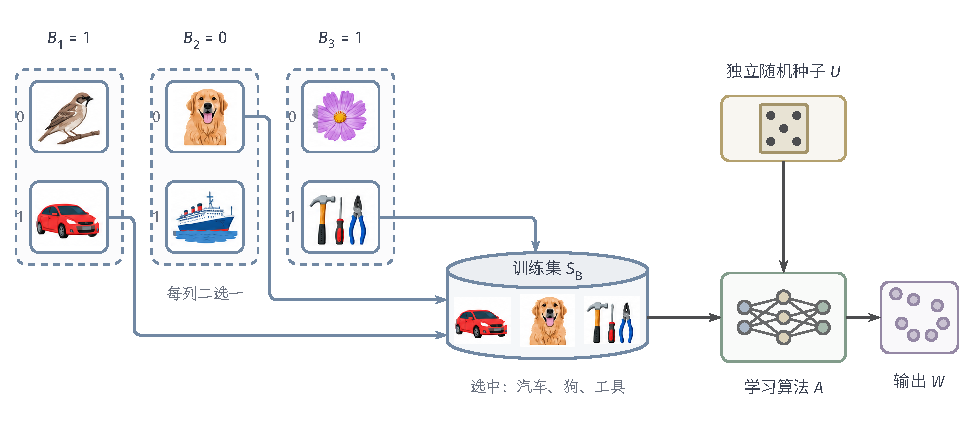
\includegraphics[width=164.600mm]{figures/06-foundations/02-learning-theory/tikz/learning-theory-conditional-information/figure.pdf}
  \caption{条件互信息的抽样构造。每列有两个独立观测，上、下分别编号0、1；选择变量决定哪一个进入训练样本。图中$\bm B=(1,0,1)$，箭头与训练样本中的内容同时标出选中的观测。算法接收选中的三个观测与独立随机种子$U$；条件互信息衡量已知全部六个观测时，输出对选择变量揭示了多少信息。}
 \label{fig:conditional-information}
\end{figure*}

\begin{definition}[算法的条件互信息量]
\label{def:algorithm-cmi}
在上述构造下，算法在分布$\mathcal P$下的\term{条件互信息}量定义为$\kappa_n(A,\mathcal P)=I(W;\bm B\mid\tilde S)$。若存在不依赖分布的$\kappa_n$，使所有允许分布满足$\kappa_n(A,\mathcal P)\leq\kappa_n$且$\kappa_n/n\to0$，则称算法序列具有在允许分布族上统一的条件互信息稳定性。
\end{definition}

$\bm B$共有$2^n$种取值，所以$0\leq\kappa_n(A,\mathcal P)\leq n\log2$。线性上界排除了无穷值，但它与$n$同阶，并不保证代价消失；要让泛化代价趋于零，还需证明算法实际透露的选择信息是$o(n)$。精确样本均值说明这一步并非自动成立：观测取自连续分布时，$2n$个备选值以概率1使不同选择给出不同的和，已知$\tilde S$后由$W$可以反推出全部$\bm B$，于是$\kappa_n=n\log2$，下面定理的上界停留在常数$\sqrt{2\log2}\approx1.18$。条件互信息消除了无穷值，却不能为每个泛化良好的算法给出有效的界。

\begin{theorem}[条件互信息与期望风险]
\label{thm:conditional-information-risk}
设$(Z,\mathcal Z)$与$(\mathcal W,\mathcal B_{\mathcal W})$为标准Borel空间，$\ell:\mathcal W\times Z\to[0,1]$可测，$\mathcal P$为$Z$上的概率分布，$\tilde S,\bm B,U,S_{\bm B},W$如上构造。则
\[
 \left|\mathbb E[R_{\mathcal P}(W)-\hat R_{S_{\bm B}}(W)]\right|\leq\sqrt{\frac{2\kappa_n(A,\mathcal P)}n}.
\]
\end{theorem}
\begin{proof}
用每对中未被选中的观测评价输出，并减去经验风险，记
\[
 g(\tilde S,\bm B,W)=\frac1n\sum_{i=1}^n[\ell(W,z_{i,1-B_i})-\ell(W,z_{i,B_i})].
\]
在真实联合分布$P$下，未选观测独立于训练样本和内部随机数，所以$\mathbb E_Pg=\mathbb E[R_{\mathcal P}(W)-\hat R_{S_{\bm B}}(W)]$。构造参照分布$Q$：保留$(\tilde S,W)$的联合分布，但在给定$\tilde S$后独立、均匀地重新抽取$\bm B$；于是$D_{\mathrm{KL}}(P\|Q)=\kappa_n(A,\mathcal P)$。在$Q$下，给定$\tilde S,W$，第$i$项随$B_i$以相同概率取一对相反数，绝对值不超过1，各项独立，故$\log\mathbb E_Qe^{\lambda g}\leq\lambda^2/(2n)$。将此式用于引理~\ref{lem:change-of-measure}，得$\mathbb E_Pg\leq\kappa_n/\lambda+\lambda/(2n)$，取$\lambda=\sqrt{2n\kappa_n}$；对$-g$同理。
\end{proof}

参照过程不同，常数也不同，不能通过简单替换$I(W;S)$得到。若平均经验优化误差至多$\rho_n$，风险分解给出平均超额风险界$\sqrt{2\kappa_n/n}+\rho_n$；两项若有不依赖分布的上界且$\kappa_n/n\to0$、$\rho_n\to0$，便得到PAC学习。

条件互信息的线性上界不保证代价消失，那么哪些算法确实只透露$o(n)$的选择信息？回到第~\ref{sec:sample-compression}节的压缩方案。在双样本构造中，输出由至多$k$条训练记录和$b$比特旁信息重构；给定候选池$\tilde S$后，选出这些记录只需说明“取哪几个位置、每个位置取候选对中的哪一个”，可能的描述是有限的。

\begin{theorem}[样本压缩控制条件互信息]
\label{thm:compression-conditional-information}
设$Z=X\times\{0,1\}$为标准Borel空间，$\mathcal H\subseteq\{0,1\}^X$，$(\kappa,\varrho)$是定义~\ref{def:sample-compression}中的$(k,b)$一致压缩方案，且压缩与重构映射可测。设$\mathcal P$是$\mathcal H$可实现的分布，在双样本构造中令确定性算法输出$W=\varrho(\kappa(S_{\bm B}))$。则
\[
\begin{aligned}
 \kappa_n(A,\mathcal P)=I(W;\bm B\mid\tilde S)
 &\leq b\log2+\log\sum_{j=0}^{k}\binom nj2^j\\
 &\leq b\log2+k\log(2n)+\log(k+1).
\end{aligned}
\]
\end{theorem}
\begin{proof}
可实现性保证$S_{\bm B}$以概率1可由某个$h\in\mathcal H$正确分类，此时压缩映射给出$(S_I,u)$；在概率为零的例外事件上把描述固定为某个约定值，不影响互信息。给定$\tilde S$，记$D=(I,(B_i)_{i\in I},u)$：它说明保留哪些训练位置、这些位置选中了候选对中的哪一个，以及旁信息。已知$\tilde S$与$D$就能写出保留的记录$S_I=(z_{i,B_i})_{i\in I}$，进而算出$W=\varrho(S_I,u)$，所以给定$\tilde S$后，$W$是$D$的函数。由数据处理不等式，$I(W;\bm B\mid\tilde S)\leq I(D;\bm B\mid\tilde S)\leq H(D\mid\tilde S)$。$D$至多取$\sum_{j\leq k}\binom nj2^j\cdot2^b$个值，离散变量的熵不超过其取值个数的对数，即得第一个不等式。再由$\binom nj2^j\leq(2n)^j\leq(2n)^k$与$k+1$项求和，得到第二个不等式。
\end{proof}

证明中位置集合$I$可以依赖全部训练记录，包括未保留的那些；这种依赖已经包含在对$D$全部可能取值的计数中。重构器只能读取描述$D$所指的记录和旁信息；若算法另有独立随机种子，先条件于种子再计数。无旁信息的基本结果来自Steinke与Zakynthinou\scite{steinke2020conditional}，有限旁信息的项由同一描述计数补入。代入定理~\ref{thm:conditional-information-risk}，有界损失下期望泛化差至多$\sqrt{2(b\log2+k\log(2n)+\log(k+1))/n}$。阈值方案$k=1$、$b=0$、$n=100$时，组合数和为$1+2n=201$，右侧约为$\sqrt{2\times5.30/100}\approx0.33$。

两种用途要分开。第~\ref{sec:sample-compression}节的一致压缩界在可实现、零一损失条件下直接控制风险，同样$n=100$时以95\%的概率风险至多约$0.077$，速率为$\log n/n$；本节的界在一般有界损失下控制期望泛化差，速率为$\sqrt{\log n/n}$，不重复前节的分类证明。压缩是控制条件互信息的一种具体途径，但反过来，单凭条件互信息较小，不能反推出同样规模的精确样本重构方案。连续样本均值则说明另一种可能：精确均值要用到全部记录，已知候选池后可能揭示全部选择。条件互信息与可学习性之间的构造性联系，留到第~\ref{sec:stability-characterization}节建立共同的子采样构造以后统一说明。

\subsubsection{PAC--Bayes的先验、后验与风险界}
\label{sec:pac-bayes}

互信息界控制的是对训练集取平均的偏差。若想对这一次抽到的训练集给出高概率结论，可以换一个参照对象：不再比较输出与样本的联合分布和乘积分布，而比较依赖样本的输出分布与一个在抽样前固定的分布。设算法根据样本$S$在决策空间上得到一个分布$Q_S$，预测时先从$Q_S$抽取一个完整决策，再用它预测。训练前就认为很可能的决策，选中它们几乎不需要付出代价；训练前认为不太可能的决策，选中它们就要付出较大代价。这正是PAC--Bayes的比较方式。

先用有限候选看清这种代价从哪里来。设损失取值于$[0,1]$，候选规则有限或可数，训练前给每个规则$h$分配权重$P(h)>0$，$\sum_hP(h)=1$。把总失败概率$\delta$按$\delta P(h)$分给各规则：对固定的$h$，Hoeffding不等式说$R_{\mathcal P}(h)>\hat R_S(h)+\sqrt{\log(1/(\delta P(h)))/(2n)}$的概率至多$\delta P(h)$。对全部规则求并，失败概率合计至多$\delta$，于是以至少$1-\delta$的概率，所有规则同时满足
\begin{equation}
 R_{\mathcal P}(h)\leq\hat R_S(h)+\sqrt{\frac{\log(1/P(h))+\log(1/\delta)}{2n}}.
 \label{eq:prior-weighted-union-bound}
\end{equation}
因为同时成立，看过样本后选中的规则也适用。选择先验权重很小的规则，要支付更大的$\log(1/P(h))$。取$n=1000$、$\delta=0.05$：均匀先验分给$1024$个候选时，每个规则的附加项为$\sqrt{(\log1024+\log20)/2000}\approx0.071$；若先验把一半权重给某个规则，它的附加项降到$\sqrt{(\log2+\log20)/2000}\approx0.043$，其余规则的附加项则变大。先验权重规定的是分析中的参照与失败预算，不表示规则正确的概率；它必须在看样本前确定，否则预算分配本身就依赖了样本。

下面从选一个规则推广到选一个规则上的分布。

\begin{definition}[PAC--Bayes的先验与后验]
\label{def:pac-bayes-distributions}
设$\mathcal W$为可测决策空间。先验$P_0$是与样本$S$独立的$\mathcal W$上概率分布，后验$Q_S$是由$S$决定的$\mathcal W$上概率分布。对于任意分布$Q$，定义
\[
 \hat R_S(Q)=\mathbb E_{w\sim Q}\hat R_S(w),\qquad R(Q)=\mathbb E_{w\sim Q}R_{\mathcal P}(w).
\]
\end{definition}

“后验”在此只表示依赖数据的分布，不要求按贝叶斯公式求出。$R(Q)$是先从$Q$抽取完整决策、再计算损失后的平均，它通常不等于“平均参数”或“平均预测器”的风险。看一个离散例子：两个候选决策的经验错误率分别为$0.02$和$0.10$，后验赋予它们概率$0.9$和$0.1$，随机预测器的经验错误率为$0.9\times0.02+0.1\times0.10=0.028$。若先验对两者各赋$1/2$，信息代价为$D_{\mathrm{KL}}(Q\|P_0)=0.9\log1.8+0.1\log0.2\approx0.368$；若后验把全部概率都给第一个决策，经验错误率降到$0.02$，信息代价却升到$\log2\approx0.693$。经验风险评价预测，相对熵评价概率质量重新分配了多少，PAC--Bayes界在两者之间权衡。一般地，$N$个候选的均匀先验下，把全部质量集中到一个候选需支付$\log N$，保持$Q=P_0$则代价为零。后验取点质量$\delta_h$时，$D_{\mathrm{KL}}(\delta_h\|P_0)=\log(1/P_0(h))$，正是式~\eqref{eq:prior-weighted-union-bound}中的选择代价。推广到一般决策空间时，相对熵按Radon--Nikodym导数定义，需要$Q\ll P_0$。

PAC--Bayes界要比较$\hat R_S(Q)$与$R(Q)$这两个$[0,1]$中的数。把它们看作两枚硬币正面朝上的概率，用两个Bernoulli分布之间的相对熵衡量差距：
\[
 \operatorname{kl}(a\|b)=a\log\frac ab+(1-a)\log\frac{1-a}{1-b},
\]
端点取连续延拓。当$b\in(0,1)$固定且$a$接近$b$时，它的二阶项为$(a-b)^2/[2b(1-b)]$。保留kl形式可以直接反解风险的允许区间；若使用$\operatorname{kl}(a\|b)\geq2(a-b)^2$，会得到较易计算的平方根形式，但丢失了关于两概率位置的部分信息：经验风险接近0时，kl形式给出的风险界接近$1/n$量级，平方根形式只有$1/\sqrt n$量级，下文的数值例子会比较二者。

\begin{theorem}[PAC--Bayes期望风险界]
\label{thm:pac-bayes-bound}
设$(Z,\mathcal Z)$为可测观测空间，$\mathcal P$为其上的概率分布，$(\mathcal W,\mathcal B_{\mathcal W})$为可测决策空间，损失$\ell:\mathcal W\times Z\to[0,1]$联合可测。令$S\sim\mathcal P^n$，$n\geq1$，先验$P_0$为与$S$独立的$\mathcal W$上概率分布。对于任意$\delta\in(0,1)$，以至少$1-\delta$的概率，所有满足$Q\ll P_0$的分布$Q$同时满足
\begin{equation}
 \operatorname{kl}\bigl(\hat R_S(Q)\|R(Q)\bigr)\leq\frac{D_{\mathrm{KL}}(Q\|P_0)+\log((n+1)/\delta)}{n}.
 \label{eq:pac-bayes-kl}
\end{equation}
从而在同一事件上，
\[
 R(Q)\leq\hat R_S(Q)+\sqrt{\frac{D_{\mathrm{KL}}(Q\|P_0)+\log((n+1)/\delta)}{2n}}.
\]
\end{theorem}

证明要解决的难点是：后验$Q$依赖样本，不能直接对它使用只适用于固定决策的集中不等式。办法分三步。先对每个固定决策控制经验风险偏离期望风险的指数矩；再对与样本无关的先验求平均，用Markov不等式得到一个只由样本决定的高概率事件；最后在这个事件上，用引理~\ref{lem:change-of-measure}把先验下的平均换成任意后验下的平均，代价正是相对熵。由于高概率事件不依赖$Q$，结论对所有后验同时成立，后验可以在看过样本后再选。先验平均与后验平均之间的转换产生了相对熵项，这一步不是把单规则的界按后验简单平均：单规则界的附加项$\sqrt{\log(1/P_0(h))}$按$Q$平均以后，一般不等于相对熵。

\begin{proof}
固定决策$w$，记其期望风险为$r$。若$r=0$或$r=1$，有界损失几乎处处为相应常量，经验风险也等于$r$，下面的指数矩等于1。以下设$0<r<1$。若单样本损失为Bernoulli变量，经验风险为$k/n$的概率是$\binom nk r^k(1-r)^{n-k}$，而$e^{n\operatorname{kl}(k/n\|r)}=(k/n)^k(1-k/n)^{n-k}/[r^k(1-r)^{n-k}]$，故
\[
 \mathbb E_S e^{n\operatorname{kl}(\hat R_S(w)\|r)}
 =\sum_{k=0}^n\binom nk\left(\frac kn\right)^k\left(1-\frac kn\right)^{n-k}\leq n+1.
\]
每一项都是成功概率为$k/n$的二项分布取值于$k$的概率，因而不超过1。对一般$[0,1]$损失，可依次对每个损失变量条件化：固定其余变量后，所用指数矩关于当前取值是凸函数；把取值在$[0,1]$内的变量按其条件均值换成只取0和1的Bernoulli变量，会使凸函数的期望不减小。逐坐标重复这一步，便把一般有界损失化为前面的Bernoulli情形。

对独立先验积分，并交换积分次序（被积函数非负），得
\[
 \mathbb E_S\mathbb E_{w\sim P_0}e^{n\operatorname{kl}(\hat R_S(w)\|R_{\mathcal P}(w))}\leq n+1.
\]
Markov不等式给出：以至少$1-\delta$的概率，
\[
 \mathbb E_{w\sim P_0}e^{n\operatorname{kl}(\hat R_S(w)\|R_{\mathcal P}(w))}\leq\frac{n+1}{\delta}.
\]
在这个只由样本决定的事件上，对任意$Q\ll P_0$且$D_{\mathrm{KL}}(Q\|P_0)<\infty$（相对熵无穷时结论平凡），取非负函数$g(w)=n\operatorname{kl}(\hat R_S(w)\|R_{\mathcal P}(w))$应用引理~\ref{lem:change-of-measure}：
\begin{equation}
 \mathbb E_Q g\leq D_{\mathrm{KL}}(Q\|P_0)+\log\mathbb E_{P_0}e^g\leq D_{\mathrm{KL}}(Q\|P_0)+\log\frac{n+1}\delta.
 \label{eq:change-of-measure}
\end{equation}
由$\operatorname{kl}$的联合凸性和Jensen不等式，左侧不小于$n\operatorname{kl}(\hat R_S(Q)\|R(Q))$，即得第一式。最后使用$\operatorname{kl}(a\|b)\geq2(a-b)^2$得到第二式。
\end{proof}

Maurer的精细指数矩估计可在相应条件下把$n+1$换成$2\sqrt n$\scite{maurer2004pacbayes}。若后验满足$D_{\mathrm{KL}}(Q_S\|P_0)\leq K$，要使经验风险外的代价不超过$\varepsilon$，可直接要求
\begin{equation}
 2n\varepsilon^2\geq K+\log((n+1)/\delta).
 \label{eq:pac-bayes-sample-requirement}
\end{equation}
忽略$n$的对数，充分样本量随$(K+\log(1/\delta))/\varepsilon^2$增长。如果后验的平均经验风险为零，可利用$\operatorname{kl}(0\|r)=-\log(1-r)$，在同一事件中得到
\[
 R(Q_S)\leq1-\exp\left(-\frac{K+\log((n+1)/\delta)}n\right)\leq\frac{K+\log((n+1)/\delta)}n.
\]
例如$K=5$、$n=1000$、$\delta=0.05$时，$\log(1001/0.05)\approx9.90$，零经验风险下风险至多约$0.0149$，平方根形式则只给出$\sqrt{14.9/2000}\approx0.086$。注意零经验风险要求整个后验平均为零，单个中心决策分类正确尚不足以使用这一速率。

PAC--Bayes界本身只是风险上界。后验经验风险与先验代价需要共同控制：把后验铺得更宽可以让它更接近先验、降低信息代价，却可能覆盖到经验风险较高的决策；把后验收窄到训练所得中心附近可以保持低经验风险，信息代价却会上升。图~\ref{fig:lt7a-pac-bayes-tradeoff}在$d=20$维中计算这一权衡。先验$P_0=\mathcal N(\bm0,\bm I_d)$，后验$Q_\sigma=\mathcal N(\hat{\bm w},\sigma^2\bm I_d)$，$\|\hat{\bm w}\|_2=2$；由两个各向同性高斯分布的相对熵公式，
\[
 D_{\mathrm{KL}}(Q_\sigma\|P_0)=\frac{\|\hat{\bm w}\|_2^2}2+\frac d2\bigl(\sigma^2-1-\log\sigma^2\bigr),
\]
第一项是中心离先验均值多远，第二项是后验宽度与先验宽度不一致的代价，后者乘着维数$d$。设经验风险在中心附近按$0.05+0.05\|\bm w-\hat{\bm w}\|_2^2$增长（教学构造），则后验平均经验风险为$0.05+0.05d\sigma^2=0.05+\sigma^2$。取$n=1000$、$\delta=0.05$：$\sigma=0.6$时经验风险$0.41$、相对熵约$5.8$，宽后验的代价在经验风险；$\sigma=0.05$时经验风险$0.053$、相对熵约$51.9$，窄后验的代价在信息；平方根形式的上界在$\sigma\approx0.13$处最小，约为$0.21$。

\begin{figure*}[htbp]
 \centering
 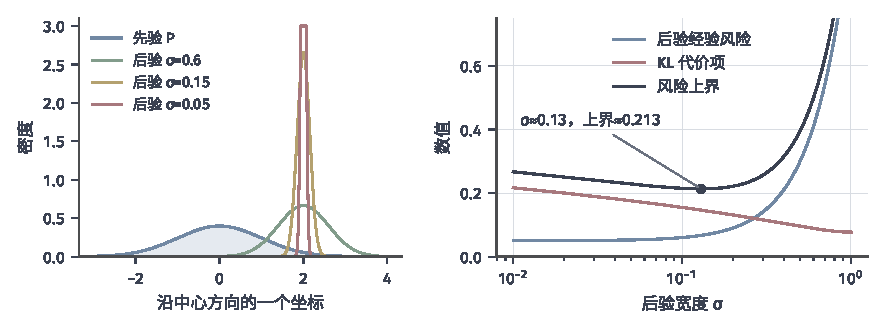
\includegraphics[width=150mm]{figures/06-foundations/02-learning-theory/matplotlib/lt7a-pac-bayes-tradeoff/figure.pdf}
 \caption{PAC--Bayes中经验风险与相对熵代价的权衡。左：沿中心方向的一个坐标上，先验$\mathcal N(0,1)$（浅蓝）与中心位于2、宽度$\sigma=0.6,0.15,0.05$的后验密度（纵轴截到3）。右：$d=20$、$\|\hat{\bm w}\|_2=2$、$n=1000$、$\delta=0.05$时，后验经验风险$0.05+0.05d\sigma^2$（教学构造）、平方根形式的代价项与二者之和随$\sigma$的变化，黑点为上界最小处。数据见图源目录。}
 \label{fig:lt7a-pac-bayes-tradeoff}
\end{figure*}

这一权衡说明了权重调整的实际作用：后验可以偏向训练表现好的决策，但更集中的调整要付出更大的信息代价，评价时须把经验风险与代价放在一起。因此，风险上界与完整学习结论是两回事。相对于比较决策空间的学习保证，还需证明算法能找到经验表现足够好、且信息代价随样本量增长足够慢的后验；这一步由具体算法和模型结构决定。对神经网络，高斯扰动后的经验风险、平坦性与参数化的关系，以及具体后验的构造，在第~\ref{sec:network-pac-bayes}节展开。
\subsubsection{互信息与PAC--Bayes的关系}
\label{sec:information-pac-bayes-relation}

互信息与PAC--Bayes都用相对熵支付样本依赖的代价，但参照对象不同：前者以乘积分布为参照，后者以样本独立的先验为参照。两种代价之间有一个平均意义上的联系。固定样本独立先验$P_0$，令$W\mid S\sim Q_S$，平均后验$\bar Q=\mathbb E_SQ_S$即$W$的边缘分布。在相关相对熵有限时，
\begin{equation}
 \mathbb E_SD_{\mathrm{KL}}(Q_S\|P_0)=I(W;S)+D_{\mathrm{KL}}(\bar Q\|P_0).
 \label{eq:pac-bayes-information-decomposition}
\end{equation}
将对数密度比$\log(\mathrm dQ_S/\mathrm dP_0)$分成$\log(\mathrm dQ_S/\mathrm d\bar Q)$与$\log(\mathrm d\bar Q/\mathrm dP_0)$，先对$Q_S$再对$S$平均，第一部分正是$D_{\mathrm{KL}}(P_{S,W}\|P_S\otimes P_W)$，第二部分只依赖$W$的边缘分布，即得此式。第一项衡量输出平均从这一份具体样本中获取了多少信息；第二项衡量平均输出分布与先验差多远，与具体样本无关，先验恰好取为$\bar Q$时为零。由于第二项非负，平均PAC--Bayes代价不小于互信息。若先验含独立随机性，应先条件于它再陈述此式。这一等式联系的是平均量，并没有把互信息给出的期望保证变成对每份样本都成立的高概率保证。

用第~\ref{sec:generalization-tools}节开头的硬币例子核对。令后验为点质量，$Q_S=\delta_{h_0}$或$\delta_{h_1}$按多数标签选择，平均后验$\bar Q$对两者各赋$1/2$。若先验取$P_0=\bar Q$，每份样本的代价都是$\log2$，平均代价$\log2$恰好等于$I(W;S)$，第二项为零。若先验改为把$0.9$的权重给$h_0$，两种样本上的代价分别为$\log(1/0.9)\approx0.105$与$\log(1/0.1)\approx2.303$，平均为$1.204$；其中$I(W;S)=\log2\approx0.693$不变，其余$0.511$正是$D_{\mathrm{KL}}(\bar Q\|P_0)=\frac12\log\frac{0.5}{0.9}+\frac12\log\frac{0.5}{0.1}$。先验选得不好，PAC--Bayes就为平均输出分布与先验的偏离额外付费。

这一分解说明，不能把后验—先验的相对熵直接称为样本—输出互信息：前者还包含平均输出分布与所选先验的偏离。两种界的保证对象也不同。互信息界（定理~\ref{thm:mutual-information-risk}）控制对样本与内部随机性平均后的泛化差；PAC--Bayes界（定理~\ref{thm:pac-bayes-bound}）给出对这一次训练集以高概率成立、同时适用于全部后验的不等式，需要损失有界、$Q\ll P_0$及相应的可测性。二者各自保留这些条件，平均意义上的联系不能把一种保证换成另一种。这些分布比较都没有考察相邻训练集上输出怎样变化，下一小节建立这种扰动实验。

\subsection{输出的扰动敏感性：算法稳定性}
\label{sec:algorithmic-stability}

压缩与信息方法考察输出与整份样本的关系；稳定性直接做一个替换实验。取一条训练观测$z_i$，把它换成独立的新观测后重新训练。原来的$z_i$没有参与新模型的训练，因此可以独立地评价新模型；如果这次替换只让模型在$z_i$上的损失改变很小，原模型在$z_i$上的训练评价就接近一次独立评价。训练损失偏乐观，是因为算法用这些观测挑选了输出，输出可能恰好迁就了它们；稳定性先解除某个观测与模型的训练依赖，再控制解除依赖所造成的损失变化。\term{算法稳定性}（algorithmic stability）描述的正是训练数据变化对输出的影响。这一推理只涉及算法实际产生的输出，不需要估计决策空间中其他决策的风险：第~\ref{sec:real-valued-classes}节的两个ERM面对同一个决策空间，只因为并列最优者的选择方式不同，期望风险就完全不同。

用均值估计先看清“单个观测的影响”：$[0,1]$上的$n$个数替换一个，均值至多改变$1/n$；用平方损失在同一区间评价时，由$|(w-z)^2-(w'-z)^2|=|w-w'|\,|w+w'-2z|\leq2|w-w'|$，损失至多改变$2/n$。这个计算展示一条观测的影响怎样被其余样本分摊，也说明从参数变化转到损失变化需要利用损失的性质。本小节依次回答四个问题：怎样改变样本并度量损失变化；这种控制支持什么风险评价；何时足以建立学习保证；具体算法怎样验证这些条件。替换与删除是两种样本操作，均匀与平均是两种控制方式，二者属于不同的划分，可以组合。共同子采样构造只在第~\ref{sec:stability-characterization}节证明一次，小节末再比较压缩、信息与稳定性。

\subsubsection{样本变更与稳定性定义}

固定算法序列$(A_n)_{n\geq1}$及损失。令$S=(z_1,\ldots,z_n)\sim\mathcal P^n$，$z_i'\sim\mathcal P$独立于$S$。$S^{(i)}$表示把$z_i$替换为$z_i'$后的样本，它保持样本量$n$；$S^{\setminus i}$表示删除$z_i$后的样本，样本量变为$n-1$。两份样本若只有一项不同，称为相邻样本。定义稳定性时，除了样本操作，还要确定在哪个观测上比较两次输出的损失：可以是任意测试观测、被替换出去的观测$z_i$，或被删除的观测$z_i$。不同的选择给出不同的条件。

图~\ref{fig:learning-stability}画出替换实验：两份样本共享其余$n-1$项，算法设置也相同，只替换一项；两次输出在同一测试点上计算损失，再比较差值。如果替换使某个测试点上的损失大幅改变，说明算法的输出对该观测很敏感。

\begin{figure*}[htbp]
  \centering
  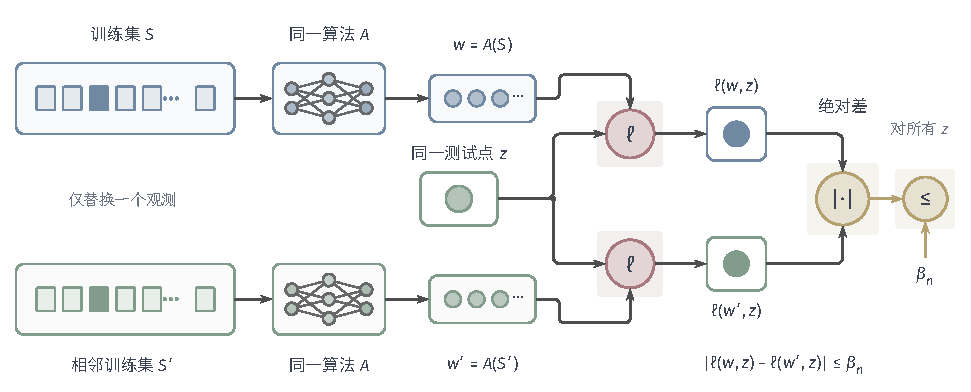
\includegraphics[width=164.600mm]{figures/06-foundations/02-learning-theory/tikz/learning-theory-stability/figure.pdf}
  \caption{算法稳定性的相邻样本实验。两批样本只替换一个观测，同一算法分别输出$\bm w=A(S)$与$\bm w'=A(S')$。两次输出在同一测试点$z$上计算损失，再比较绝对差；均匀稳定性要求所有这样的损失差都不超过$\beta_n$。图中的比较对象是损失，不是参数距离。}
  \label{fig:learning-stability}
\end{figure*}

先看确定性算法。要求对最不利的情形成立，就得到均匀条件；把最坏情形换成按样本出现概率的平均，就得到平均条件。

\begin{definition}[均匀稳定性]
\label{def:uniform-stability}
若对任意只相差一个观测的$s,s'\in Z^n$和任意$z\in Z$都有
\begin{equation}
 |\ell(A_n(s),z)-\ell(A_n(s'),z)|\leq\beta_n,
 \label{eq:uniform-stability}
\end{equation}
则称算法具有$\beta_n$\term{均匀稳定性}（uniform stability）。
\end{definition}

\begin{definition}[平均稳定性]
\label{def:on-average-stability}
设$U$为独立于所有观测的算法内部随机数，$S,z_i',S^{(i)}$如上，并满足后文的稳定性可积性条件。定义
\begin{equation}
 \gamma_n(A,\mathcal P)
 =\frac1n\sum_{i=1}^n\mathbb E_{S,z_i',U}
 \left[\ell(A_n(S^{(i)},U),z_i)-\ell(A_n(S,U),z_i)\right].
 \label{eq:on-average-stability}
\end{equation}
给定$\bar\beta_n(\mathcal P)\geq0$，若$\gamma_n(A,\mathcal P)\leq\bar\beta_n(\mathcal P)$，则称算法在分布$\mathcal P$下具有速率$\bar\beta_n(\mathcal P)$的\term{平均稳定性}（on-average stability）。若对所有允许分布均有$\gamma_n(A,\mathcal P)\leq\bar\beta_n$且$\bar\beta_n$不依赖$\mathcal P$，则称算法具有速率$\bar\beta_n$的在允许分布族上统一的平均稳定性。
\end{definition}

两种定义的评价点不同。均匀稳定性在任意测试观测上比较，平均稳定性在被替换出去的$z_i$上比较：$A(S)$在训练中见过$z_i$，$A(S^{(i)})$没见过它，二者在$z_i$上的损失差衡量“用$z_i$训练”带来的平均优势。平均定义取有符号的差，不同样本上的增加和减少可以抵消；它只限制平均意义下训练带来的优势，不限制每次替换的绝对变化，这里采用的一侧约定与《Understanding Machine Learning》第13章一致\scite{shalevshwartz2014}。先对每项取绝对值再平均，得到平均绝对变化，是更强的要求。均匀条件蕴含平均绝对变化不超过$\beta_n$，从而蕴含平均条件；反方向一般不成立，因为平均小只说明大变化出现的概率小，不能推出每次变化都小。

删除操作给出留一法的条件。删除$z_i$后用其余$n-1$项重新训练，再在$z_i$上评价：$z_i$没有参与$A_{n-1}(S^{\setminus i})$的训练，它对这个输出而言相当于一条独立的新观测。

\begin{definition}[留一法风险估计]
\label{def:loo-risk}
对确定性学习算法序列$(A_n)_{n\geq1}$，$n\geq2$时的留一法风险估计定义为
\[
 \hat R_S^{\mathrm{loo}}(A)=\frac1n\sum_{i=1}^n\ell(A_{n-1}(S^{\setminus i}),z_i).
\]
\end{definition}

\begin{definition}[平均留一法稳定性]
\label{def:loo-stability}
若对每个允许分布$\mathcal P$都有
\[
 \frac1n\sum_{i=1}^n\mathbb E_{S\sim\mathcal P^n}
 \left|\ell(A_n(S),z_i)-\ell(A_{n-1}(S^{\setminus i}),z_i)\right|
 \leq\beta_n^{\mathrm{loo}},
\]
则称算法序列具有速率$\beta_n^{\mathrm{loo}}$的在允许分布族上统一的平均\term{留一法稳定性}（leave-one-out stability）。
\end{definition}

这个条件只在被删观测上评价损失，并对样本和删除位置取平均绝对差；它允许个别样本或位置上出现较大变化，不要求对任意测试点都有同一个上界。留一法稳定性还有概率型和二阶矩型的定义，这里采用平均绝对差版本\scite{bousquetelisseeff2002}。注意两个算法的样本量不同：比较的是$A_n$与$A_{n-1}$。

对随机算法$A(S,U)$，要明确哪些期望包含内部随机数，以及绝对值放在期望内部还是外部。本章的均匀条件先对内部随机性取平均，再比较：
\[
 \sup_{s,s'\text{相邻},\,z\in Z}
 \left|\mathbb E_U\ell(A_n(s,U),z)-\mathbb E_U\ell(A_n(s',U),z)\right|\leq\beta_n,
\]
其中$U$与样本独立，且对每个固定的$s,z$，$\ell(A_n(s,U),z)$关于$U$可积。这是“期望差的绝对值”，弱于“绝对差的期望”：两次随机运行各自可以相差很大，只要平均损失接近即可。后面的存在性定理正使用这个较弱的形式，不能把它改成绝对差的期望。另一方面，验证强控制时常用的做法是在两份相邻样本上共享同一个$U$（同一初始化、同一索引序列），这时$\mathbb E_U|\ell(A(s,U),z)-\ell(A(s',U),z)|$小就足以推出上式；共享随机数是一种耦合手段，不自动构成定义。留一法稳定性也可以先对内部随机性平均，再比较删除前后的损失绝对差。

回到入口的均值计算，用刚建立的定义辨认它属于哪种控制：平方损失下的$2/n$界对任意相邻样本与任意测试观测成立，所以是$2/n$均匀稳定性。先看更简单的绝对损失。设$z_i\in[0,1]$，算法输出$A(S)=\bar z$，用绝对损失$\ell(w,z)=|w-z|$评价。替换一项后，两个均值之差为$(z_i'-z_i)/n$，绝对值至多$1/n$；在同一个测试观测$z$处，由反三角不等式
\[
 \bigl||\bar z-z|-|\bar z'-z|\bigr|\leq|\bar z-\bar z'|\leq\frac1n,
\]
所以均值算法具有$1/n$均匀稳定性。图~\ref{fig:lt7a-mean-replacement-stability}取$S=(0.1,0.3,0.4,0.8,0.9)$，均值为$0.5$；把$0.9$换成$0$，均值变为$0.32$，两次输出相距$0.18\leq1/5$。左图两条V形损失曲线之间的带宽处处不超过$0.18$，在$z$远离两个均值时恰好达到它。删除也可直接计算：$\bar z-\bar z_{-i}=(z_i-\bar z_{-i})/n$，删去$0.9$后$\bar z_{-5}=0.4$，差为$(0.9-0.4)/5=0.1$，于是$\beta_n^{\mathrm{loo}}\leq1/n$。这两个计算只检验了稳定性；均值是否使绝对损失的期望最小是另一个问题，这里不作此断言。

\begin{figure*}[htbp]
 \centering
 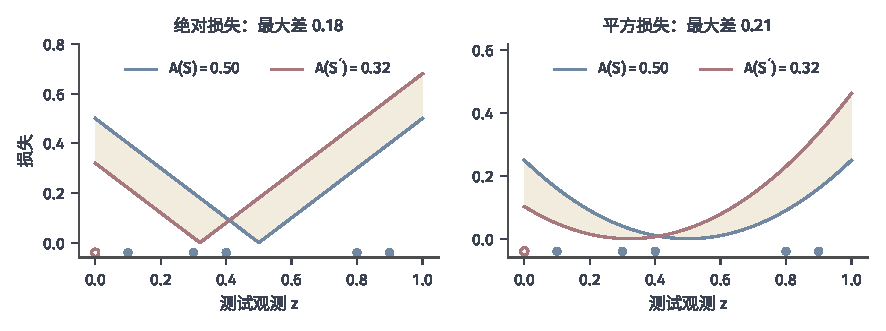
\includegraphics[width=150mm]{figures/06-foundations/02-learning-theory/matplotlib/lt7a-mean-replacement-stability/figure.pdf}
 \caption{替换一个样本后两次均值输出的损失差。样本$(0.1,0.3,0.4,0.8,0.9)$（蓝点）的均值为$0.50$，把$0.9$换成$0$（空心点）后均值为$0.32$。横轴为测试观测$z$，两条曲线分别是两次输出的损失，黄色带宽为损失差。左：绝对损失，最大差$0.18$，不超过$1/n=0.2$；右：平方损失，最大差约$0.21$，不超过$2/n=0.4$。图为解析教学构造。}
 \label{fig:lt7a-mean-replacement-stability}
\end{figure*}

替换与删除不能直接互推。例如，算法按样本量的奇偶输出两个不同常量：替换一项不改变样本量，输出不变，均匀稳定性常数为零；删除一项使样本量奇偶改变，输出可能在每个位置都跳变，删除条件失败。反过来，有一个单向的关系。

\begin{lemma}[均匀删除稳定性推出替换稳定性]
\label{lem:deletion-to-replacement-stability}
若确定性算法对任意$s\in Z^n$、任意位置$i$与任意测试观测$z\in Z$都满足$|\ell(A_n(s),z)-\ell(A_{n-1}(s^{\setminus i}),z)|\leq\beta_n^{\mathrm{del}}$，则它具有$2\beta_n^{\mathrm{del}}$均匀稳定性。
\end{lemma}
\begin{proof}
设$s,s'$只在第$i$项不同。两份样本都删去第$i$项后得到同一份$n-1$项样本$s^{\setminus i}=s'^{\setminus i}$。经这份共同样本比较，三角不等式给出$|\ell(A_n(s),z)-\ell(A_n(s'),z)|\leq|\ell(A_n(s),z)-\ell(A_{n-1}(s^{\setminus i}),z)|+|\ell(A_{n-1}(s'^{\setminus i}),z)-\ell(A_n(s'),z)|\leq2\beta_n^{\mathrm{del}}$。
\end{proof}

引理要求删除控制对任意测试点成立。若只有定义~\ref{def:loo-stability}那种仅在被删点评价的平均条件，被删点在$s$与$s'$中不同，无法经共同样本比较，这一关系不再适用。

均值例子也能比较最坏情形与依赖方差的平均代价。改回平方损失$\ell(w,z)=(w-z)^2$，$z\in[0,1]$的均值为$\mu$、方差为$\sigma^2$，入口的计算给出均匀稳定性上界$2/n$；图~\ref{fig:lt7a-mean-replacement-stability}右侧的最大差约$0.21$确在$0.4$之内。下一小节的恒等式将算出平均稳定性的精确值$\gamma_n=2\sigma^2/n$，观测几乎恒定时远小于$2/n$。
\subsubsection{稳定性与风险评价}
\label{sec:on-average-stability}

下面的期望运算需要明确的可积性条件。令$z,z_i'\sim\mathcal P$且独立于$S,U$。对实际使用的样本量和允许分布，独立测试损失$\ell(A_n(S,U),z)$、训练损失$\ell(A_n(S,U),z_i)$和替换损失$\ell(A_n(S^{(i)},U),z_i)$都要求可积；删除型结论还要求$\ell(A_{n-1}(S^{\setminus i},U),z_i)$可积；使用固定比较决策$w$时要求$\ell(w,z)$可积。若用到经验风险的下确界，要求它可测且几乎处处为有限实数；期望风险的下确界要求为有限实数。后文把这组条件统称为“稳定性可积性条件”。损失有界时，这些条件自动成立。

第一个结论是一个恒等式：平均替换损失差恰好等于\term{期望泛化差}
\[
 \mathbb E_{S,U}[R_{\mathcal P}(A(S,U))-\hat R_S(A(S,U))].
\]
它为正时，经验风险平均而言低估了期望风险。

\begin{theorem}[平均稳定性与期望风险]
\label{thm:on-average-generalization}
设$(Z,\mathcal Z)$与$(\mathcal W,\mathcal B_{\mathcal W})$为可测空间，$\ell:\mathcal W\times Z\to\mathbb R$可测，$\mathcal P$为$Z$上的概率分布。令$S=(z_1,\ldots,z_n)\sim\mathcal P^n$，令$z_1',\ldots,z_n'\sim\mathcal P$彼此独立并独立于$S$，以$S^{(i)}$表示用$z_i'$替换$z_i$所得的样本。令内部随机数$U$独立于所有观测，可测算法$A:Z^n\times\mathcal U\to\mathcal W$输出$A(S,U)$，并满足稳定性可积性条件。则
\begin{equation}
 \mathbb E_{S,U}\left[R_{\mathcal P}(A(S,U))-\hat R_S(A(S,U))\right]
 =\gamma_n(A,\mathcal P).
 \label{eq:on-average-generalization-identity}
\end{equation}
因此，若$\gamma_n(A,\mathcal P)\leq\bar\beta_n(\mathcal P)$，则$\mathbb E_{S,U}R_{\mathcal P}(A(S,U))\leq\mathbb E_{S,U}\hat R_S(A(S,U))+\bar\beta_n(\mathcal P)$。
\end{theorem}
\begin{proof}
替换后，$S^{(i)}$仍由$n$个独立同分布的观测组成，而且独立于被替换出去的$z_i$。给定$S^{(i)}$和$U$时，对$z_i$取期望得到$\mathbb E_{z_i}\ell(A(S^{(i)},U),z_i)=R_{\mathcal P}(A(S^{(i)},U))$。再利用$S^{(i)}$与$S$同分布，得到$\mathbb E\ell(A(S^{(i)},U),z_i)=\mathbb E_{S,U}R_{\mathcal P}(A(S,U))$。另一方面，$n$个原观测上的损失平均恰好是经验风险，故$\frac1n\sum_i\mathbb E\ell(A(S,U),z_i)=\mathbb E_{S,U}\hat R_S(A(S,U))$。两式相减即得恒等式。
\end{proof}

证明中，被替换出去的$z_i$同时扮演两个角色：对$A(S)$它是训练点，对$A(S^{(i)})$它是独立测试点。交换$z_i$与$z_i'$不改变全部独立观测的联合分布，平均替换损失差因此就是期望泛化差。恒等式说的是多次抽样并重新训练后的平均关系：为正表示经验评价平均偏低，为负表示平均偏高；不同样本上的正负偏差可以抵消，单次训练的泛化差仍可能很大，绝对泛化差的平均也未必小。若速率只对某个固定分布成立，结论也只限于该分布。

用平方损失下的均值估计核对恒等式。第~\ref{sec:information-stability}节已经直接算出这个算法的期望泛化差为$2\sigma^2/n$，所以$\gamma_n=2\sigma^2/n$；也可以按定义逐项计算替换损失差，得到同一结果。方差越小，平均替换带来的损失变化越小；观测恒定时为零。只知道取值范围时，由$\sigma^2\leq1/4$得到分布无关上界$1/(2n)$，仍比均匀界$2/n$小四倍：平均分析利用了最坏情形分析没有使用的方差信息。

均匀稳定性同时控制期望泛化差的两侧。

\begin{theorem}[均匀稳定性与期望风险]
\label{thm:stability-expected-generalization}
在定理~\ref{thm:on-average-generalization}的设定下，若确定性算法$A$具有$\beta_n$均匀稳定性，则
\begin{equation}
 \left|\mathbb E_S\left[R_{\mathcal P}(A(S))-\hat R_S(A(S))\right]\right|\leq\beta_n.
 \label{eq:stability-expectation-bound}
\end{equation}
对随机算法，若内部随机性平均后的均匀条件成立，则同一结论对$\mathbb E_{S,U}$成立。
\end{theorem}
\begin{proof}
由式~\eqref{eq:on-average-generalization-identity}，左侧绝对值内等于$\gamma_n(A,\mathcal P)$，即$\ell(A(S^{(i)}),z_i)-\ell(A(S),z_i)$按样本与位置的平均。$S$与$S^{(i)}$相邻，均匀稳定性给出每一项的绝对值至多$\beta_n$。随机算法时，先对$U$取期望再用内部平均后的条件。
\end{proof}

式~\eqref{eq:stability-expectation-bound}的绝对值在期望外面，既不是绝对泛化差的平均值，也不保证每份样本上泛化差都小；随机算法的结论针对样本和内部随机性共同平均，不保证每次随机运行都稳定。

删除操作给出另一种风险评价。

\begin{theorem}[留一法稳定性与期望风险]
\label{thm:loo-risk}
设$(Z,\mathcal Z)$与$(\mathcal W,\mathcal B_{\mathcal W})$为可测空间，$\ell$可测，确定性算法$A_k:Z^k\to\mathcal W$对每个$k\geq1$均可测。固定$n\geq2$和分布$\mathcal P$，令$S\sim\mathcal P^n$，并假定$\ell(A_n(S),z_i)$与$\ell(A_{n-1}(S^{\setminus i}),z_i)$对每个$i$均可积。则对$T\sim\mathcal P^{n-1}$，
\[
 \mathbb E_S\hat R_S^{\mathrm{loo}}(A)=\mathbb E_TR_{\mathcal P}(A_{n-1}(T)),
\]
且若平均留一法稳定性的左侧至多$\beta_n^{\mathrm{loo}}$，则
\[
 \left|\mathbb E_T R_{\mathcal P}(A_{n-1}(T))-\mathbb E_S\hat R_S(A_n(S))\right|\leq\beta_n^{\mathrm{loo}}.
\]
\end{theorem}
\begin{proof}
被删去的$z_i$独立于$S^{\setminus i}$。固定$S^{\setminus i}$后对$z_i$取期望，第$i$项变成$R_{\mathcal P}(A_{n-1}(S^{\setminus i}))$；而$S^{\setminus i}$由$n-1$个独立同分布观测组成，与$T$同分布。对$i$平均得到第一式。两侧减去$\mathbb E_S\hat R_S(A_n(S))$，三角不等式把差控制为各项删除前后损失绝对差的平均，至多$\beta_n^{\mathrm{loo}}$。
\end{proof}

定理联系的是两种评价：$n$项样本上的经验评价，和用$n-1$项样本训练后的总体评价。少一项正是为了让评价点独立于训练，所以它没有直接给出$A_n$自身的期望泛化差，不能把留一估计未经转换地当作同一模型的风险。

若只想在给定的一份样本上用经验风险估计期望风险，就需要控制泛化差在样本间的随机波动。损失有界且算法均匀稳定时，替换一项对泛化差的影响有统一上界，可以用有界差分不等式。

\begin{theorem}[均匀稳定性的高概率泛化界]
\label{thm:stability-high-probability}
在定理~\ref{thm:stability-expected-generalization}的设定下，设损失取值于$[0,1]$，确定性算法具有$\beta_n$均匀稳定性。则任意$\delta\in(0,1)$下，以至少$1-\delta$的样本概率，
\[
 |R_{\mathcal P}(A(S))-\hat R_S(A(S))|
 \leq\beta_n+(2n\beta_n+1)\sqrt{\frac{\log(2/\delta)}{2n}}.
\]
\end{theorem}
\begin{proof}
记$g(S)=R_{\mathcal P}(A(S))-\hat R_S(A(S))$。替换一个观测后，期望风险变化至多$\beta_n$；经验风险的$n-1$个共同观测各变化至多$\beta_n/n$，合计不超过$\beta_n$，被替换项变化至多$1/n$。因此$|g(S)-g(S')|\leq2\beta_n+1/n$。对$n$个独立观测应用双侧有界差分不等式，$|g(S)-\mathbb Eg(S)|$以至少$1-\delta$的概率不超过$(2\beta_n+1/n)\sqrt{n\log(2/\delta)/2}=(2n\beta_n+1)\sqrt{\log(2/\delta)/(2n)}$。再使用$|\mathbb E g(S)|\leq\beta_n$即得结论。
\end{proof}

当$\beta_n=O(1/n)$时，右侧第二项为$O(1/\sqrt n)$，整个界趋于零；均值例子中$\beta_n=1/n$，$n=1000$、$\delta=0.05$时界约为$0.001+3\times0.043\approx0.13$。若只有$\beta_n=1/\sqrt n$，第二项不再下降，界失去作用：有界差分不等式把$n$个替换影响平方相加，$\beta_n$必须远小于$1/\sqrt n$才能被吸收。更精细的集中分析给出$|R_{\mathcal P}(A(S))-\hat R_S(A(S))|\leq C(\beta_n\log(2n)\log(2/\delta)+\sqrt{\log(2/\delta)/n})$，其中$C$是通用常数；这是Bousquet、Klochkov与Zhivotovskiy的结果，其高阶矩证明不在此展开\scite{bousquet2020sharper}。对随机算法，这些结论只适用于内部随机性平均后的损失；评价单次随机运行的输出，还需另外控制内部随机性造成的波动。无论哪种形式，风险评价都只说明经验风险可信，尚未保证经验目标已经优化充分。
\subsubsection{稳定性与可学习性}
\label{sec:stability-characterization}

期望泛化差小，只说明重复抽样、训练后的两种平均风险接近，它们仍可能同时很大：在$[0,1]$上用平方损失，若观测恒为1而算法始终输出0，训练风险与期望风险都是1，泛化差为零，而输出1的风险为零。以比较决策空间的风险下确界为基准，还需要算法在训练样本上接近经验最优，即\term{经验优化误差}（empirical optimization error）$\hat R_S(A(S,U))-\inf_{w\in\mathcal W}\hat R_S(w)$要小；上例中它恒为1。第~\ref{sec:risk-comparison}节的期望比较（定理~\ref{thm:expected-risk-comparison}）把两项合并：对固定的、不依赖样本的$w$，经验风险是期望风险的无偏估计，加入并减去经验风险即得平均超额风险的上界。这一比较对数据依赖的输出不能直接使用无偏性，正是需要稳定性的原因。下面写出它与稳定性结合的形式。

\begin{theorem}[稳定性与经验最优性给出超额期望风险]
\label{thm:generalization-optimization-learning}
\label{thm:stability-excess-risk}
设$\mathcal W$非空，算法输出$A_n(S,U)\in\mathcal W$，满足稳定性可积性条件。若对所有允许分布，期望泛化差至多$g_n$、平均经验优化误差至多$\rho_n$，其中$g_n,\rho_n$为不依赖分布的非负数，则\term{超额期望风险}满足
\begin{equation}
 \mathbb E_{S,U}R_{\mathcal P}(A_n(S,U))-\inf_{w\in\mathcal W}R_{\mathcal P}(w)\leq g_n+\rho_n.
 \label{eq:generalization-optimization-learning}
\end{equation}
特别地，取$g_n$为平均稳定性速率$\bar\beta_n$（定理~\ref{thm:on-average-generalization}）或均匀稳定性速率$\beta_n$（定理~\ref{thm:stability-expected-generalization}），得到
\begin{equation}
 \mathbb E_{S,U}R_{\mathcal P}(A_n(S,U))-\inf_{w\in\mathcal W}R_{\mathcal P}(w)\leq\bar\beta_n+\rho_n.
 \label{eq:stability-excess-risk}
\end{equation}
若右侧趋于零，则算法相对于允许族统一地PAC学习此问题；$g_n+\rho_n\leq\varepsilon\delta$足以使超额风险超过$\varepsilon$的概率不超过$\delta$。允许族包含全部相关分布时，这才是分布无关的PAC学习。
\end{theorem}
\begin{proof}
式~\eqref{eq:generalization-optimization-learning}即定理~\ref{thm:expected-risk-comparison}在当前记号下的结论：对任意不依赖样本且风险有限的$w$，期望风险差分解为期望泛化差、经验风险之差与$\mathbb E[\hat R_S(w)-R_{\mathcal P}(w)]=0$三项，第二项不超过平均经验优化误差，再对$w$取下确界。由于输出属于$\mathcal W$，超额风险$X=R_{\mathcal P}(A(S,U))-\inf_wR_{\mathcal P}(w)$非负；Markov不等式给出$\mathbb P\{X>\varepsilon\}\leq(g_n+\rho_n)/\varepsilon$。
\end{proof}

由平均界转成概率结论时，Markov不等式只能用于非负的超额风险，不能直接用于可正可负的泛化差。固定分布下的速率只给出该分布下的保证；两项上界在允许族上统一时，才得到相对于该族的统一PAC结论。平方损失下的均值估计：样本均值恰好是经验最优解，$\rho_n=0$，上式给出平均超额风险至多$2\sigma^2/n$；直接计算得到精确值$\mathbb E(\bar z-\mu)^2=\sigma^2/n$，二者同阶，稳定性常数宽松一倍。由$\sigma^2\leq1/4$，$n\geq1/(2\varepsilon\delta)$足以满足这条分析给出的PAC要求。第~\ref{sec:real-valued-classes}节反例中始终输出$w_0$的算法，在任何相邻样本上输出都相同，$\beta_n=0$，经验优化误差也为零，于是立即得到学习保证；一致收敛失败的原因是那些集合决策的风险难以估计，而稳定性只检查算法实际选择的$w_0$。

前面回答的是“给定一个算法，怎样验证它能学习”。反过来问：只要问题可学习，能否构造出一个既稳定、经验风险又接近最优的算法？回答这个问题时，要把经验最优性加强为对每份样本都成立。

\begin{definition}[始终渐近经验风险最小化]
\label{def:aerm}
设随机算法$A(S,U)$的输出属于$\mathcal W$，$U$独立于样本。若存在$\rho_n\to0$，使任意$S\in Z^n$均满足
\[
 \mathbb E_U\hat R_S(A(S,U))-\inf_{w\in\mathcal W}\hat R_S(w)\leq\rho_n,
\]
则称$A$为始终渐近经验风险最小化算法（always AERM）。
\end{definition}

“始终”限定的对象是样本：每一份样本都必须满足同一个$\rho_n$上界，只对内部随机性取平均。若只在允许分布下对样本取期望后才满足不依赖分布的速率，则称为在允许分布族上统一的AERM，条件较弱。“渐近”指允许经验风险略高于最低值，只要差距随样本量趋于零；这容纳了只求近似解的算法。下面的刻画使用更强的始终AERM\scite{shalevshwartz2010learnability}。

与二分类对照：二分类中可学习、VC维有限与一致收敛三者等价；一般损失下一致收敛不再必要，起刻画作用的是“存在稳定且始终渐近经验最优的算法”。刻画可学习性的不再是决策空间的某种容量，而是某个算法的行为。

\begin{theorem}[一般学习基本定理：均匀稳定性与可学习性]
\label{thm:general-stability-characterization}
设$(Z,\mathcal Z)$与$(\mathcal W,\mathcal B_{\mathcal W})$为可测空间，$\mathcal W$非空，$\ell:\mathcal W\times Z\to[0,1]$可测，并允许$Z$上的所有概率分布。对每个$n$，假定$s\mapsto\inf_{w\in\mathcal W}\hat R_s(w)$可测；随机算法均由可测映射$A_n:Z^n\times\mathcal U\to\mathcal W$表示，其内部随机数$U$与样本独立。则以下两个命题等价：
\begin{enumerate}
 \item 存在随机算法$(B_n)$，使任意$\varepsilon,\delta\in(0,1)$都有不依赖$\mathcal P$的$n_0(\varepsilon,\delta)$，并且所有$n\geq n_0$与$Z$上的每个概率分布$\mathcal P$均满足
 \[
  \mathbb P_{S,U}\!\left\{R_{\mathcal P}(B_n(S,U))-\inf_{w\in\mathcal W}R_{\mathcal P}(w)\leq\varepsilon\right\}\geq1-\delta;
 \]
 \item 存在随机算法$(A_n)$及不依赖$\mathcal P$的非负序列$\rho_n\to0$、$\beta_n\to0$，使每份$s\in Z^n$都满足$\mathbb E_U\hat R_s(A_n(s,U))-\inf_{w}\hat R_s(w)\leq\rho_n$，而任意只相差一个观测的$s,s'\in Z^n$及任意$z\in Z$都满足
 \[
  \left|\mathbb E_U\ell(A_n(s,U),z)-\mathbb E_U\ell(A_n(s',U),z)\right|\leq\beta_n.
 \]
\end{enumerate}
\end{theorem}
\begin{proof}
命题2蕴含命题1：定理~\ref{thm:stability-expected-generalization}给出$g_n=\beta_n$；始终AERM对每份样本成立，取期望后给出平均经验优化误差至多$\rho_n$；再由定理~\ref{thm:generalization-optimization-learning}得到PAC保证。

逆向从已有学习算法$B$出发。构造的想法是：只让$B$看样本中随机抽出的一小部分。抽出的项数$k$要随$n$增长，$B$才能学好；又要满足$k/n\to0$，被替换的那一项才很少被看到，输出才稳定。$k=\lfloor\sqrt n\rfloor$同时满足两点。

先把$B$的PAC保证改写成随样本量趋于零的期望界。因为损失有界，超额风险按PAC成功和失败事件分开：成功时至多$\varepsilon$，失败时至多1，故期望至多$\varepsilon+\delta$。PAC保证对每一对$(\varepsilon,\delta)$各给一个门槛，构造则需要一列随样本量$k$趋于零、且不依赖分布的期望界$a_k$。对每个整数$r\geq1$，选门槛$N_r$，使$k\geq N_r$时取$\varepsilon=\delta=1/r$可得期望超额风险至多$2/r$。令$N'_r=\max\{r,N_1,\ldots,N_r\}$；这组门槛单调且$N'_r\geq r$，所以集合$\{r:N'_r\leq k\}$有限。该集合非空时，令$r(k)$为其中的最大等级并取$a_k=2/r(k)$；在它为空的有限前缀取平凡界$a_k=1$。任意固定等级最终都会进入集合，故$r(k)\to\infty$、$a_k\to0$，而这个上界对全部分布统一成立。

再构造新算法。对输入$S$，有放回地独立抽取$k=\lfloor\sqrt n\rfloor$个位置$J=(J_1,\ldots,J_k)$，将对应序列$T$交给$B$；若$B$还使用随机数$U_0$，新算法的随机数就是$U=(J,U_0)$。固定$S$后，$T$独立取自经验分布$\mathcal P_S=n^{-1}\sum_i\delta_{z_i}$，其中$\delta_{z_i}$为点质量分布。由于$R_{\mathcal P_S}(w)=\hat R_S(w)$，$B$在这一分布上的学习保证给出
\[
 \mathbb E_{J,U_0}\hat R_S(B(T,U_0))-\inf_w\hat R_S(w)\leq a_k.
\]
经验分布可以来自任意$S$，因此新算法对每份样本都满足AERM，且$\rho_n=a_k\to0$。这一步用到命题1对全部分布成立：必要性的证明需要把经验分布也纳入允许族。

最后验证稳定性。在相邻样本上共享索引$J$及随机数$U_0$，两次输出只有访问被替换位置时才可能不同。$k$次抽取中至少一次抽到该位置的概率至多$k/n$，损失变化至多1，所以$\beta_n\leq k/n\leq1/\sqrt n\to0$。构造的算法同时满足稳定性与始终AERM，逆向因此成立。
\end{proof}

必要性的证明构造了一个新的算法，说明可学习时存在一个稳定的学习算法，并不证明原来的每个成功算法都稳定；有放回子采样只用于存在性证明，不追求最优的样本效率或计算效率。证明还依赖允许全部分布，结论不能无条件推广到任意受限分布族：受限族可能不含经验分布。平均条件弱于均匀条件，但在算法存在性的意义上二者给出相同的刻画。

\begin{theorem}[一般学习基本定理的平均稳定性形式]
\label{thm:average-stability-characterization}
在定理~\ref{thm:general-stability-characterization}的条件下，该问题分布无关PAC可学习，当且仅当存在随机算法$(A_n)$以及不依赖$\mathcal P$的非负序列$\rho_n\to0$、$\bar\beta_n\to0$，使每份$s\in Z^n$都满足$\mathbb E_U\hat R_s(A_n(s,U))-\inf_w\hat R_s(w)\leq\rho_n$，并且$Z$上的每个概率分布都满足$\gamma_n(A_n,\mathcal P)\leq\bar\beta_n$。
\end{theorem}
\begin{proof}
充分性由定理~\ref{thm:on-average-generalization}与定理~\ref{thm:generalization-optimization-learning}给出。必要性：前一定理的子采样算法均匀稳定且始终AERM，而均匀稳定性蕴含平均稳定性，同一个算法满足这里的条件。
\end{proof}

这里的等价是针对问题的：存在一组算法满足平均条件，与存在一组算法满足均匀条件相互等价，两边可以使用不同的算法。固定某一个算法后，平均稳定性不能升级为均匀稳定性，一侧的平均保证也不能升级为逐样本保证。
第~\ref{sec:conditional-information}节留下了一个问题：条件互信息与可学习性有什么构造性联系？定理~\ref{thm:general-stability-characterization}证明中的子采样算法同时给出答案。它只把被抽到的至多$k$个位置交给原算法，而抽样索引与样本独立；在双样本构造中，给定候选池、索引和原算法的随机数后，输出至多揭示这$k$个位置的二元选择。
\begin{theorem}[条件互信息稳定性与可学习性]
\label{thm:conditional-information-learning}
设$(Z,\mathcal Z)$与$(\mathcal W,\mathcal B_{\mathcal W})$为标准Borel空间，其余条件同定理~\ref{thm:general-stability-characterization}。则该问题分布无关PAC可学习，当且仅当存在随机算法$(A_n)$以及不依赖$\mathcal P$的非负序列$\rho_n\to0$与$\kappa_n$（$\kappa_n/n\to0$），使每份$s\in Z^n$都满足$\mathbb E_U\hat R_s(A_n(s,U))-\inf_w\hat R_s(w)\leq\rho_n$，并且$Z$上每个概率分布都满足$\kappa_n(A_n,\mathcal P)\leq\kappa_n$。
\end{theorem}
\begin{proof}
充分性由定理~\ref{thm:conditional-information-risk}与定理~\ref{thm:generalization-optimization-learning}给出。必要性使用定理~\ref{thm:general-stability-characterization}证明中的子采样算法，它已满足始终AERM，这里只需估计它的选择信息。记抽样索引为$J=(J_1,\ldots,J_k)$、$k=\lfloor\sqrt n\rfloor$，原学习算法的随机数为$U_0$。给定$\tilde S,J,U_0$时，输出仅由被访问位置的选择变量$(B_{J_1},\ldots,B_{J_k})$决定，每个选择变量至多包含$\log2$的信息，故
\[
 I(W;\bm B\mid\tilde S)\leq I(W,J,U_0;\bm B\mid\tilde S)=I(W;\bm B\mid\tilde S,J,U_0)\leq k\log2.
\]
等式使用$J,U_0$与$\tilde S,\bm B$独立；最后一步使用互信息不超过决定输出的离散选择变量的熵。因此可取$\kappa_n=k\log2$，有$\kappa_n/n\to0$。
\end{proof}

这个界比定理~\ref{thm:compression-conditional-information}对一般压缩的计数更紧：那里保留哪些位置由样本决定，描述中要计入$\log\binom nk$量级的位置选择；这里索引独立于样本，条件于它以后只剩$k$个二元选择，每个至多$\log2$。取$k=\lfloor\sqrt n\rfloor$，条件互信息与样本量之比$k\log2/n$和稳定性代价$k/n$同时趋于零。充分性方向把统一的次线性条件互信息与经验优化误差合并，需要的是信息量与样本量之比趋零，不要求信息量本身趋零。

这里的必要性同样允许重新构造算法，并不要求每个成功算法本身的条件互信息都小。这一刻画也不能换成普通互信息版本，因为后者仍会记录连续观测的无限精度：子采样算法把选中的连续观测交给原算法时，普通互信息可能仍是无穷。

留一法给出充分结论的一个变式，它用$A_n$的经验优化误差与平均删除稳定性控制$A_{n-1}$的风险。

\begin{theorem}[留一法稳定性与可学习性]
\label{thm:loo-learning}
在定理~\ref{thm:loo-risk}的设定下，设$\mathcal W$非空，每个固定$w$的损失可积，出现的风险下确界为有限实数且可测。若存在不依赖$\mathcal P$的非负数$\beta_n^{\mathrm{loo}},\rho_n$，使平均留一法稳定性的左侧至多$\beta_n^{\mathrm{loo}}$，并且$\mathbb E_S[\hat R_S(A_n(S))-\inf_w\hat R_S(w)]\leq\rho_n$，则对$T\sim\mathcal P^{n-1}$，
\[
 \mathbb E_T R_{\mathcal P}(A_{n-1}(T))-\inf_{w\in\mathcal W}R_{\mathcal P}(w)\leq\beta_n^{\mathrm{loo}}+\rho_n.
\]
若$\beta_n^{\mathrm{loo}}\to0$且$\rho_n\to0$，则该算法序列PAC学习此问题。使用$m$个观测达到精度$\varepsilon$与置信度$1-\delta$的一个充分条件是$\beta_{m+1}^{\mathrm{loo}}+\rho_{m+1}\leq\varepsilon\delta$。
\end{theorem}
\begin{proof}
对任意不依赖样本的$w$，经验优化误差条件给出
\[
 \mathbb E_S\hat R_S(A_n(S))\leq\mathbb E_S\hat R_S(w)+\rho_n=R_{\mathcal P}(w)+\rho_n.
\]
代入定理~\ref{thm:loo-risk}，再对$w$取下确界，得到超额风险的期望上界。对非负的超额风险应用Markov不等式，令$m=n-1$即得所述样本量条件。
\end{proof}

实际使用$m$项样本时，对应条件来自$m+1$项算法的稳定性和经验误差，删除操作的索引不能在学习结论中被抹去。
\subsubsection{损失稳定性的验证}
\label{sec:parameter-stability}

前三小节的条件都直接比较损失，但具体算法的分析通常先得到两次训练输出之间的距离，再估计损失差。本小节给出两条转换：一条比较参数向量，另一条比较完整随机决策的输出分布。它们只把“距离小”转换成“损失变化小”，具体算法的距离及速率由第~\ref{sec:regularized-learning}节和第~\ref{sec:gradient-descent-guarantees}节给出；一个假设的距离上界本身不表示某个算法已经满足它。

\paragraph{参数距离与Lipschitz转换}

本段令$\mathcal W\subseteq\mathbb R^d$，用欧氏范数度量参数向量；换一种参数表示或距离，条件本身也会改变。两次运行共享同一个内部随机数$U$，例如比较两次SGD时使用相同的初始化和样本索引序列，输出之差才反映样本替换的影响。

\begin{definition}[均匀参数稳定性]
\label{def:uniform-parameter-stability}
设算法$A(S,U)\in\mathcal W\subseteq\mathbb R^d$。若对任意相邻样本$S,S'$都有$\mathbb E_U\|A(S,U)-A(S',U)\|_2\leq\alpha_n$，则称算法具有速率$\alpha_n$的均匀\term{参数稳定性}（argument stability）。
\end{definition}

\begin{definition}[平均参数稳定性]
\label{def:average-parameter-stability}
沿用定义~\ref{def:on-average-stability}中的$S,S^{(i)}$和$U$。若
\begin{equation}
 \frac1n\sum_{i=1}^n\mathbb E_{S,z_i',U}\|A(S,U)-A(S^{(i)},U)\|_2\leq\bar\alpha_n(\mathcal P),
 \label{eq:average-parameter-stability}
\end{equation}
则称算法在分布$\mathcal P$下具有速率$\bar\alpha_n(\mathcal P)$的平均参数稳定性；同一个上界适用于所有允许分布时，称其为在允许分布族上统一的平均参数稳定性。
\end{definition}

样本均值可以直接算出参数距离：替换一项后$A(S^{(i)})-A(S)=(z_i'-z_i)/n$。在$[0,1]$上，均匀界为$1/n$，平均界为$\mathbb E|z-z'|/n$。若$z$以概率$p$取1、其余取0，两次独立取值不同的概率为$2p(1-p)$，平均界为$2p(1-p)/n$；数据几乎恒定时，它比最坏情形距离小得多。

参数距离本身不是风险量。若存在常数$L$，使任意$\bm u,\bm v\in\mathcal W$和$z\in Z$都满足
\begin{equation}
 |\ell(\bm u,z)-\ell(\bm v,z)|\leq L\|\bm u-\bm v\|_2,
 \label{eq:parameter-loss-lipschitz}
\end{equation}
则称损失关于参数是$L$-Lipschitz的：参数移动距离$r$时，同一观测上的损失至多改变$Lr$。

\begin{theorem}[参数稳定性与损失稳定性]
\label{thm:parameter-to-loss-stability}
设$\mathcal W\subseteq\mathbb R^d$配备Borel $\sigma$代数，$\ell$可测并满足式~\eqref{eq:parameter-loss-lipschitz}；比较两份样本时共享同一个$U$，且每个固定$s,z$下$\ell(A(s,U),z)$关于$U$可积。若任意相邻$s,s'$均满足$\mathbb E_U\|A(s,U)-A(s',U)\|_2\leq\alpha_n$，则任意相邻$s,s'$及任意$z$均满足
\[
 \left|\mathbb E_U\ell(A(s,U),z)-\mathbb E_U\ell(A(s',U),z)\right|\leq L\alpha_n.
\]
另一方面，固定$\mathcal P$并满足稳定性可积性条件，若式~\eqref{eq:average-parameter-stability}成立，则$|\gamma_n(A,\mathcal P)|\leq L\bar\alpha_n(\mathcal P)$。
\end{theorem}
\begin{proof}
对任意相邻样本和任意观测，Lipschitz条件给出
\[
 |\mathbb E_U\ell(A(s,U),z)-\mathbb E_U\ell(A(s',U),z)|\leq L\,\mathbb E_U\|A(s,U)-A(s',U)\|_2,
\]
代入均匀参数稳定性上界即得第一项。对定义~\ref{def:on-average-stability}中的损失差逐项取绝对值，再使用Lipschitz条件，得到
\[
 |\gamma_n(A,\mathcal P)|\leq\frac Ln\sum_i\mathbb E\|A(S^{(i)},U)-A(S,U)\|_2\leq L\bar\alpha_n(\mathcal P).
\]
\end{proof}

完成这一转换后，参数化算法也能使用前两小节的结论。

\begin{theorem}[参数稳定性与期望泛化差]
\label{thm:parameter-expected-generalization}
在定理~\ref{thm:parameter-to-loss-stability}的条件下，若式~\eqref{eq:average-parameter-stability}成立，则
\begin{equation}
 \left|\mathbb E_{S,U}[R_{\mathcal P}(A(S,U))-\hat R_S(A(S,U))]\right|\leq L\bar\alpha_n(\mathcal P).
 \label{eq:parameter-generalization}
\end{equation}
均匀参数稳定性成立时，可将$\bar\alpha_n(\mathcal P)$替换为$\alpha_n$。
\end{theorem}
\begin{proof}
由替换样本恒等式~\eqref{eq:on-average-generalization-identity}，左侧绝对值内等于$\gamma_n(A,\mathcal P)$，前一定理给出其绝对值至多$L\bar\alpha_n(\mathcal P)$。均匀界对每对相邻样本成立，取平均后仍成立，故$\bar\alpha_n(\mathcal P)\leq\alpha_n$。
\end{proof}

\begin{theorem}[均匀参数稳定性的高概率泛化界]
\label{thm:parameter-high-probability}
在定理~\ref{thm:parameter-to-loss-stability}的条件下，设损失取值于$[0,1]$，确定性算法对任意相邻$s,s'$满足$\|A(s)-A(s')\|_2\leq\alpha_n$。则以至少$1-\delta$的样本概率，
\[
 |R_{\mathcal P}(A(S))-\hat R_S(A(S))|\leq L\alpha_n+(2nL\alpha_n+1)\sqrt{\frac{\log(2/\delta)}{2n}}.
\]
\end{theorem}
\begin{proof}
由定理~\ref{thm:parameter-to-loss-stability}，该算法具有$L\alpha_n$均匀稳定性；代入定理~\ref{thm:stability-high-probability}。
\end{proof}

参数稳定并不保证算法选到了低风险决策：“观测恒为1、算法始终输出0”的例子中参数稳定性常数为零，算法却远离最优。学习保证还必须单独约束经验优化误差。

\begin{theorem}[参数稳定性与可学习性]
\label{thm:parameter-stability-learning}
设$\mathcal W\subseteq\mathbb R^d$为非空Borel决策空间，损失满足式~\eqref{eq:parameter-loss-lipschitz}，其中$L$不依赖分布或样本量；算法满足稳定性可积性条件，出现的风险下确界为有限实数且可测。若存在不依赖$\mathcal P$的非负数$\bar\alpha_n,\rho_n$，使所有允许分布满足式~\eqref{eq:average-parameter-stability}（右侧为$\bar\alpha_n$）且平均经验优化误差至多$\rho_n$，则
\[
 \mathbb E_{S,U}R_{\mathcal P}(A(S,U))-\inf_{\bm w\in\mathcal W}R_{\mathcal P}(\bm w)\leq L\bar\alpha_n+\rho_n.
\]
若$\bar\alpha_n\to0$且$\rho_n\to0$，则算法相对于允许族统一地PAC学习此问题；$L\bar\alpha_n+\rho_n\leq\varepsilon\delta$是充分样本量条件。均匀参数稳定性成立时可用$\alpha_n$替换$\bar\alpha_n$。
\end{theorem}
\begin{proof}
定理~\ref{thm:parameter-expected-generalization}给出$g_n=L\bar\alpha_n$，代入定理~\ref{thm:generalization-optimization-learning}即得。
\end{proof}

本定理通过非负的超额风险完成概率转换，与前一个高概率界的集中证明不同；只要两项都趋于零即可，不必先证明高概率界下降。继续用Bernoulli观测：$z$以概率$p$取1、其余取0，$\mathcal W=[0,1]$，平方损失在$[0,1]$上关于参数$2$-Lipschitz，平均参数距离为$2p(1-p)/n$，均值是经验最优解，故$\rho_n=0$，平均超额风险至多$4p(1-p)/n$。由$p(1-p)\leq1/4$，可取分布无关的充分样本量$n\geq1/(\varepsilon\delta)$；它比直接按损失平均得到的$2\sigma^2/n=2p(1-p)/n$宽松一倍，因为统一的Lipschitz转换没有保留平方损失的具体结构。

参数距离小并不自动意味着损失变化小。对阈值分类器$h_w(x)=\mathbb I\{x\geq w\}$，参数从$-a$移到$a$只移动$2a$，但在$(x,y)=(0,1)$处，零一损失对任意$a>0$都从0跳为1。反方向也不成立：若损失为$\ell((a,b),z)=(a-z)^2$，参数$b$完全不影响损失，任意改变$b$损失都不变。参数稳定性依赖于参数表示和距离的选择，是一条充分的分析路径，不是每个成功算法都必须满足的性质。
\paragraph{非负光滑损失的自界转换}

全局Lipschitz条件并不总能满足。以一维平方损失$\ell(w,z)=(w-z)^2/2$为例，梯度为$w-z$：残差为1时参数移动0.01，损失约变化0.01；残差为100时，同样的移动使损失约变化1。参数无界时残差可以任意大，找不到统一的Lipschitz常数。不过两处梯度之差恰为$u-v$，梯度的变化速度是固定的。若$\|\nabla\ell(\bm u,z)-\nabla\ell(\bm v,z)\|_2\leq M\|\bm u-\bm v\|_2$，称损失为$M$-光滑。光滑性本身不限制梯度大小，还要借助损失非负：非负光滑损失满足自界关系$\|\nabla\ell(\bm u,z)\|_2^2\leq2M\ell(\bm u,z)$，即损失小处梯度也小，因为梯度很大时沿负梯度走一小步就会使损失降到零以下。推导中会出现距离的平方，所以把平均参数距离加强为均方根距离
\[
 b_n^2(\mathcal P)=\frac1n\sum_{i=1}^n\mathbb E_{S,z_i',U}\|A(S^{(i)},U)-A(S,U)\|_2^2.
\]
由Cauchy--Schwarz不等式，$b_n(\mathcal P)$不小于平均参数距离，限制它是更强的要求。

\begin{theorem}[光滑损失下参数稳定性与期望泛化差]
\label{thm:smooth-parameter-generalization}
设$\mathcal W=\mathbb R^d$，$\ell:\mathbb R^d\times Z\to[0,\infty)$可测，对任意$z$，$\ell(\cdot,z)$可微且$M$-光滑，$M>0$。固定$\mathcal P$，算法满足稳定性可积性条件，$b_n(\mathcal P)<\infty$，并记$r_n=\mathbb E_{S,U}\hat R_S(A(S,U))<\infty$。则
\begin{equation}
 \mathbb E_{S,U}[R_{\mathcal P}(A(S,U))-\hat R_S(A(S,U))]\leq b_n(\mathcal P)\sqrt{2Mr_n}+\frac M2 b_n^2(\mathcal P).
 \label{eq:smooth-parameter-generalization}
\end{equation}
\end{theorem}
\begin{proof}
光滑性意味着对任意$\bm u,\bm v$都有
\[
 \ell(\bm v,z)\leq\ell(\bm u,z)+\langle\nabla\ell(\bm u,z),\bm v-\bm u\rangle+\frac M2\|\bm v-\bm u\|_2^2.
\]
令$\bm v=\bm u-\nabla\ell(\bm u,z)/M$，并利用左侧非负，得到$\|\nabla\ell(\bm u,z)\|_2^2\leq2M\ell(\bm u,z)$。再令$\bm u=A(S,U)$、$\bm v=A(S^{(i)},U)$，对$z_i$使用同一个光滑性不等式，左侧减去$\ell(\bm u,z_i)$后正是替换样本恒等式中的第$i$项损失差，右侧是一个内积项和一个距离平方项。对样本、替换观测、内部随机数和位置取平均，内积项先用Cauchy--Schwarz不等式拆成梯度与距离两部分，再用自界关系，至多为
\[
 \left(\frac1n\sum_i\mathbb E\|\nabla\ell(A(S,U),z_i)\|_2^2\right)^{1/2}b_n(\mathcal P)\leq\sqrt{2Mr_n}\,b_n(\mathcal P).
\]
二次项平均为$Mb_n^2(\mathcal P)/2$。代入恒等式~\eqref{eq:on-average-generalization-identity}即得结论。
\end{proof}

这个界不要求凸性，它用实际的平均经验风险$r_n$控制梯度大小。参数扰动不变时，$r_n$越小，右侧越小；若降低训练损失的同时$b_n(\mathcal P)$增大，就必须同时计算二者，不能只凭经验风险下降推断泛化改善。它是一侧的期望泛化差上界。

\begin{theorem}[光滑损失下参数稳定性与可学习性]
\label{thm:smooth-parameter-learning}
在定理~\ref{thm:smooth-parameter-generalization}的条件下，设$M$不依赖分布或样本量，每个固定$\bm w$的损失可积，风险下确界为有限实数且可测。若存在不依赖分布的非负序列$b_n,c_n,\rho_n$，使所有允许分布均满足$b_n(\mathcal P)\leq b_n$、$r_n\leq c_n$，且平均经验优化误差至多$\rho_n$，则
\[
 \mathbb E_{S,U}R_{\mathcal P}(A(S,U))-\inf_{\bm w\in\mathbb R^d}R_{\mathcal P}(\bm w)\leq b_n\sqrt{2Mc_n}+\frac M2b_n^2+\rho_n=:q_n.
\]
若$q_n\to0$，则算法相对于允许族统一地PAC学习此问题；$q_n\leq\varepsilon\delta$是充分样本量条件。
\end{theorem}
\begin{proof}
定理~\ref{thm:smooth-parameter-generalization}给出$g_n=b_n\sqrt{2Mc_n}+Mb_n^2/2$，代入定理~\ref{thm:generalization-optimization-learning}即得。
\end{proof}

例如$M$固定且$c_n\leq C<\infty$时，只要$b_n\to0$且$\rho_n\to0$，就有$q_n\to0$；若$c_n$随$n$增长，还需$b_n\sqrt{c_n}\to0$。光滑性可以代替全局Lipschitz条件，但转换后的界保留了损失规模这一项。

\paragraph{输出分布的Wasserstein转换}

有些算法输出的是完整决策上的分布：先由样本得到$Q_S$，预测时再抽取$w\sim Q_S$。此时可以比较两份相邻样本产生的两个输出分布。逐个配对比较两次随机输出往往没有自然的配对方式，\term{Wasserstein距离}允许先选一种最省力的配对，再计算配对后决策的平均距离。设$(\mathcal W,\mathrm d)$为完备可分度量空间，$\mu,\nu$为其上具有有限一阶矩的概率分布，一阶Wasserstein距离为
\[
 W_1(\mu,\nu)=\inf_{\pi\in\Pi(\mu,\nu)}\mathbb E_{(w,w')\sim\pi}\mathrm d(w,w'),
\]
其中$\Pi(\mu,\nu)$是边缘分别为$\mu,\nu$的全部耦合，每个耦合就是一种搬运方案。例如在实轴上，把位于0的全部质量搬到1，距离为1；若只有一半质量需要从0搬到1、另一半不动，距离为0.5。度量空间上的距离与耦合可参考\BookChapterRef{chap:information-theory-and-statistical-geometry}{卷4《数学准备：流形、概率分布与统计推断》的“概率分布的分析与优化”章}。

\begin{theorem}[输出分布稳定性与期望泛化差]
\label{thm:distribution-stability-generalization}
设$(\mathcal W,\mathrm d)$为完备可分度量空间并配备Borel $\sigma$代数，损失$\ell:\mathcal W\times Z\to[0,1]$联合可测，且对每个$z$及任意$w,w'$都有$|\ell(w,z)-\ell(w',z)|\leq L\,\mathrm d(w,w')$。可测随机学习算法根据样本输出具有有限一阶矩的分布$Q_S$。记$R(Q)=\mathbb E_{w\sim Q}R_{\mathcal P}(w)$、$\hat R_S(Q)=\mathbb E_{w\sim Q}\hat R_S(w)$。若任意相邻样本$S,S'$都满足$W_1(Q_S,Q_{S'})\leq\alpha_n$，则
\[
\begin{gathered}
 \sup_z\left|\mathbb E_{Q_S}\ell(w,z)-\mathbb E_{Q_{S'}}\ell(w,z)\right|\leq L\alpha_n,\\
 \left|\mathbb E_S[R(Q_S)-\hat R_S(Q_S)]\right|\leq L\alpha_n.
\end{gathered}
\]
进一步，若$\Theta\subseteq\mathcal W$为可测比较决策空间，$Q_S(\Theta)=1$几乎必然成立，且$\mathbb E_S[\hat R_S(Q_S)-\inf_{w\in\Theta}\hat R_S(w)]\leq\rho_n$，则$\mathbb E_SR(Q_S)-\inf_{w\in\Theta}R_{\mathcal P}(w)\leq L\alpha_n+\rho_n$；两个速率对所有允许分布统一趋于零时，得到同时包含样本与输出抽样随机性的PAC保证。
\end{theorem}
\begin{proof}
对任意耦合$\pi\in\Pi(Q_S,Q_{S'})$，$|\mathbb E_{Q_S}\ell(w,z)-\mathbb E_{Q_{S'}}\ell(w',z)|\leq\mathbb E_\pi|\ell(w,z)-\ell(w',z)|\leq L\,\mathbb E_\pi\mathrm d(w,w')$。对$\pi$取下确界得到第一式，即把“抽取$w\sim Q_S$”看作随机算法时的均匀稳定性；定理~\ref{thm:stability-expected-generalization}给出第二式。对任意固定$w\in\Theta$，近似经验最优条件给出$\mathbb E_S\hat R_S(Q_S)\leq R_{\mathcal P}(w)+\rho_n$，加上泛化差并取下确界即得超额风险界。由于$Q_S$以$\Theta$为支撑，联合随机变量$R_{\mathcal P}(w)-\inf_\Theta R_{\mathcal P}$非负，其期望不超过$L\alpha_n+\rho_n$，Markov不等式给出PAC形式。
\end{proof}

参数距离与分布距离都是证明损失变化小的中间量，验证它们是具体算法分析的任务。这里比较的是两份相邻训练集的两个输出分布；第~\ref{sec:information-stability}节的相对熵代价比较的是联合分布与乘积分布，或第~\ref{sec:pac-bayes}节中后验与样本独立的先验，参照对象不同，不能互相替代。耦合难以估计时，也可以比较相邻输出分布的总变差：$[0,1]$损失的期望差不超过它，再由$\sqrt{D_{\mathrm{KL}}(Q_S\|Q_{S'})/2}$控制；此处相对熵两端都是相邻输出分布，不能直接换成后验—先验代价。第~\ref{sec:mean-field}节把这一转换用于神经元分布。
\subsubsection{样本压缩、信息依赖与稳定性的关系}
\label{sec:stability-comparison}

现在固定同一个学习输出，按比较对象收束三条路线，图~\ref{fig:lt7-compression-information-stability}并排画出三种实验。压缩寻找足以重构输出的记录与旁信息；信息方法比较真实联合分布与消除依赖后的参照；稳定性比较相邻训练集上的损失或输出分布。前面已经证明了两处联系。第一，压缩描述可以控制条件互信息（定理~\ref{thm:compression-conditional-information}）：给定候选池后，输出只是有限个描述之一。第二，共同子采样构造同时保证了均匀稳定性与小的条件互信息（定理~\ref{thm:general-stability-characterization}与定理~\ref{thm:conditional-information-learning}）。后者依赖该构造的抽样索引与样本独立，不能由“压缩规模小”直接推出均匀稳定性：一般压缩方案的保留位置由样本决定，替换一项可能改变全部保留记录。

\begin{figure*}[htbp]
 \centering
 % 样本压缩、信息依赖与算法稳定性的三种比较实验（示意，跨栏约 165 mm）。
% 左：6 条训练记录中保留 2 条（绿圈）及旁信息 u，重构 rho(S_I,u)；其余 4 条检验重构结果。
% 中：二元观测 z 与输出 W 的联合分布（对角 0.45、非对角 0.05）与乘积分布（每格 0.25），
%     二者的相对熵即互信息 log2-h(0.1)≈0.368，与正文图 fig:lt7a-joint-product-information 相同。
% 右：相邻样本 S 与 S^{(i)} 只在第 3 项不同（红），两次输出在同一观测 z 上的损失差。
\begingroup
\providecolor{FigureGreen}{HTML}{829C8B}
\providecolor{FigureGreenFill}{HTML}{E8EEE9}
\begin{tikzpicture}[figure picture,x=1mm,y=1mm]
\tikzset{dot/.style={circle,fill=FigureBlue,inner sep=0pt,minimum size=2.6mm},
 odot/.style={circle,draw=FigureBlue,fill=white,line width=.7pt,inner sep=0pt,minimum size=2.6mm},
 box/.style={rectangle,draw=FigureStroke,fill=white,line width=.6pt,rounded corners=1mm,inner sep=2pt,font=\figurefont\footnotesize,align=center},
 cell/.style={rectangle,draw=FigureStroke,line width=.5pt,minimum width=8mm,minimum height=7mm,inner sep=0pt,font=\figurefont\footnotesize}}
% ---------- 面板 1：样本压缩
\figurePanel{0}{0}{52}{60}{样本压缩：能否重构}{FigureBlueFill}
\foreach \x/\t in {6/o,13/d,20/o,27/d,34/o,41/o}{\ifx d\t\node[dot] at (\x,44) {};\else\node[odot] at (\x,44) {};\fi}
\foreach \x in {13,27}{\draw[FigureGreen,line width=1pt] (\x,44) circle (2.6);}
\node[figure note,anchor=west] at (44,44) {$S$};
\node[box] (u) at (46,35) {$u$};
\node[box] (rec) at (26,25) {重构 $\varrho(S_I,u)$};
\draw[figure flow] (13,41)--(rec.north west);
\draw[figure flow] (27,41)--(rec.north);
\draw[figure flow] (u.south)--(rec.north east);
\node[figure note] at (26,13) {其余记录检验重构结果\\控制：描述个数\\$2^b\sum_{j\leq k}\binom nj$};
% ---------- 面板 2：信息依赖
\figurePanel{58}{0}{52}{60}{信息依赖：透露多少}{FigureYellowFill}
\node[figure note] at (71,47.5) {联合 $P_{S,W}$};
\node[figure note] at (97,47.5) {乘积 $P_S\otimes P_W$};
\node[cell,fill=FigureYellowFill] at (67,40) {$.45$}; \node[cell,fill=white] at (75,40) {$.05$};
\node[cell,fill=white] at (67,33) {$.05$}; \node[cell,fill=FigureYellowFill] at (75,33) {$.45$};
\foreach \x in {93,101}{\foreach \y in {33,40}{\node[cell,fill=FigurePaper] at (\x,\y) {$.25$};}}
\node[font=\figurefont\footnotesize] at (84,36.5) {$\|$};
\node[figure note] at (84,25) {$D_{\mathrm{KL}}=I(W;S)\approx0.368$};
\node[figure note] at (84,13) {参照：输出与样本独立\\控制：互信息、条件互信息\\或后验—先验相对熵};
% ---------- 面板 3：算法稳定性
\figurePanel{116}{0}{52}{60}{算法稳定性：换一项变多少}{FigureRedFill}
\foreach \x in {126,132,144,150}{\node[dot] at (\x,44) {}; \node[dot] at (\x,34) {};}
\node[dot] at (138,44) {};
\node[circle,fill=FigureRed,inner sep=0pt,minimum size=2.6mm] at (138,34) {};
\draw[FigureRed,line width=.6pt,dash pattern=on 1.5pt off 1pt] (138,41.4)--(138,36.6);
\node[figure note,anchor=east] at (123.5,44) {$S$};
\node[figure note,anchor=east] at (123.5,34) {$S^{(i)}$};
\node[box,anchor=west] (a1) at (154.5,44) {$A(S)$};
\node[box,anchor=west] (a2) at (154.5,34) {$A(S^{(i)})$};
\draw[figure flow] (151.8,44)--(a1.west);
\draw[figure flow] (151.8,34)--(a2.west);
\node[figure note] at (142,25) {$|\ell(A(S),z)-\ell(A(S^{(i)}),z)|\leq\beta_n$};
\node[figure note] at (142,13) {参照：相邻训练集\\控制：损失差、参数距离\\或输出分布的距离};
\end{tikzpicture}
\endgroup

 \caption{三种工具的比较实验。左：样本压缩只看保留的记录（绿圈）与旁信息$u$能否重构输出，控制对象是可能的描述个数。中：信息方法比较样本与输出的联合分布和乘积分布，这里用二元观测与以概率0.9复制它的输出，相对熵即互信息$\approx0.368$。右：稳定性替换一项（红点）后比较两次输出在同一观测上的损失。三者都用于控制经验风险与期望风险之差，前提与结论形式见表~\ref{tab:stability-object-comparison}。}
 \label{fig:lt7-compression-information-stability}
\end{figure*}

在独立同分布抽样与当前有界损失条件下，信息路线与稳定性路线还可以控制同一个平均量。由平均替换恒等式（定理~\ref{thm:on-average-generalization}），期望泛化差等于有符号的平均替换损失差$\gamma_n(A,\mathcal P)$。因此定理~\ref{thm:mutual-information-risk}也可读作$|\gamma_n(A,\mathcal P)|\leq\sqrt{I(W;S)/(2n)}$，条件互信息界同理。两条证明路线于是对同一个平均量给出上界。但这个转换只针对期望外取绝对值的有符号平均：它不把绝对值移进期望，不给出平均绝对替换变化的界，更不升级为对所有相邻样本成立的均匀保证。

这些量不能互相替换，前面的两个例子正好从相反方向说明这一点。第一个是$[0,1]$上的样本均值与平方损失：它具有$2/n$均匀稳定性，随样本量下降；但输出精确记录了连续观测的平均，普通互信息为无穷，条件互信息为$n\log2$；要从记录恢复精确均值也必须用到全部$n$条记录。它区分了“对单个观测不敏感”与“不透露精确信息”。第二个反过来。取$z_i\in\{0,1\}$，算法仅当样本全为1时输出$W=1$，否则输出0，以$\ell(w,z)=w$评价。它可由一条记录重构：样本中有0就保留一个0，全为1就保留一个1，重构时输出所保留记录的值。输出只有两种，$I(W;S)\leq\log2$，条件互信息同样至多$\log2$；但把全1样本中的任一项换成0，输出从1变为0，损失改变1，均匀稳定性常数无法随$n$下降。小压缩规模与小信息量都不保证最坏样本上的稳定性：信息代价只控制平均依赖，不控制每一对相邻样本。这个重构例子也没有提供低经验风险：若分布只产生1，训练样本必为全1，算法输出1，损失恒为1，而决策0的损失恒为0；此时输出在该分布下是常量，互信息为零，却远离最优。小压缩规模与小互信息都不能弥补经验优化的失败，不能据此宣称已经学到低风险决策。

本章用到的分布比较有三种，参照对象各不相同。互信息比较样本—输出的真实联合分布与消除依赖后的乘积分布，条件互信息比较的则是已知备选观测时选择变量的联合分布与独立重抽的参照；二者都给出期望泛化差。PAC--Bayes比较依赖样本的后验与抽样前固定的先验，给出对这一次训练集以高概率成立、且同时适用于全部后验的界。分布稳定性比较相邻训练集产生的两个输出分布，属于本小节的扰动实验，给出期望泛化差。第~\ref{sec:information-pac-bayes-relation}节的分解联系了前两种比较的平均代价；但联系平均量时，仍要逐一核对期望与高概率、整体分布与最坏样本这些量词。它们都出现分布、相对熵或距离，却不能只因此判定条件等价：后验离先验很近，并不意味着替换一个样本后后验几乎不变；反之亦然。

定理~\ref{thm:general-stability-characterization}、定理~\ref{thm:average-stability-characterization}和定理~\ref{thm:conditional-information-learning}分别用均匀稳定、平均稳定和条件互信息稳定的始终AERM算法刻画可学习性，都是算法存在性的结论；留一法稳定性、参数稳定性、分布稳定性、普通互信息与PAC--Bayes则提供验证具体算法的充分途径，不能转化为每个成功算法都必须满足的性质。表~\ref{tab:stability-object-comparison}汇总各条件直接比较的对象与进入学习保证还需要的条件，图~\ref{fig:learning-risk-routes}比较它们与一致收敛共同的证明目标。三条路线各自提供统计控制；进入第~\ref{sec:learning-algorithm-guarantees}节以后，还要对具体算法验证经验拟合与实际求解的条件。

\begin{table*}[htbp]
 \centering
 \footnotesize
 \begin{tabularx}{\linewidth}{@{}l l X X X@{}}
  \toprule
  \textbf{条件} & \textbf{样本操作或参照} & \textbf{直接比较对象} & \textbf{结论形式} & \textbf{进入学习保证还需什么} \\
  \midrule
  一致样本压缩 & 固定描述后的剩余观测 & 保留记录与旁信息的描述个数 & 高概率（可实现、零一损失） & 训练一致、对全部可实现样本统一的规模 \\
  互信息 & 乘积分布 & $I(W;S)$或$I(W;z_i)$ & 期望 & 有界或次高斯损失，以及经验最优性 \\
  条件互信息 & 双样本逐位选择 & 已知备选观测时揭示的选择信息 & 期望 & 有界损失；刻画还需始终AERM \\
  PAC--Bayes & 样本独立先验 & $D_{\mathrm{KL}}(Q\|P_0)$ & 高概率，同时适用于全部后验 & 有界损失、绝对连续；能找到经验风险低且代价受控的后验 \\
  均匀稳定性 & 替换一项 & 任意测试观测上的损失差 & 期望；损失有界时高概率 & 经验最优性；刻画还需始终AERM \\
  平均稳定性 & 替换一项 & 被替换出的$z_i$上的有符号损失差 & 期望（恒等式） & 允许族上的统一速率与经验最优性 \\
  留一法稳定性 & 删除一项 & 被删观测上的损失 & 期望；$A_{n-1}$的风险 & 经验最优性；注意$n$与$n-1$的错位 \\
  参数或分布稳定性 & 替换一项 & 共享随机数下的参数距离或$W_1$距离 & 期望；均匀时高概率 & Lipschitz或自界关系转换为损失，以及经验最优性 \\
  \bottomrule
 \end{tabularx}
 \caption{样本压缩、信息与稳定性条件的对象与保证接口，按三条路线分组。除正文已证明的联系（压缩控制条件互信息；子采样构造同时满足稳定性与小条件互信息；期望泛化差可由信息量或平均稳定性控制）外，表中条件之间不存在一般的强弱关系。}
 \label{tab:stability-object-comparison}
\end{table*}

\begin{figure*}[htbp]
  \centering
  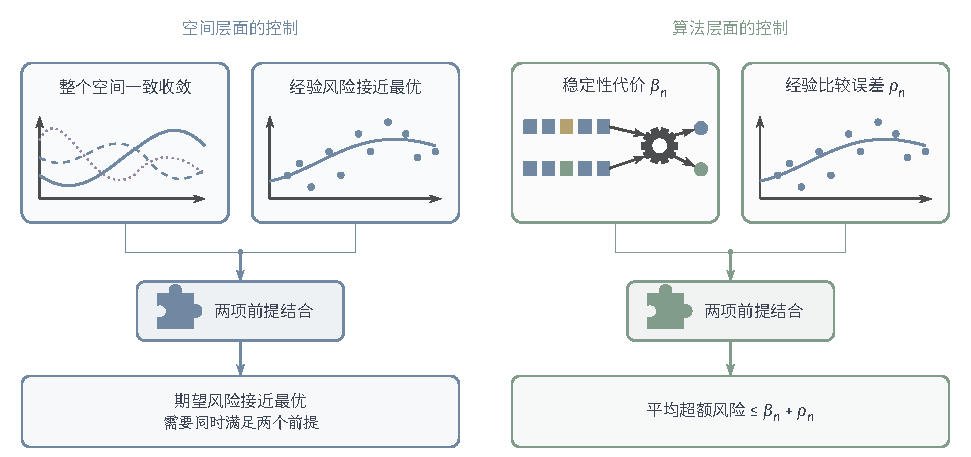
\includegraphics[width=164.600mm]{figures/06-foundations/02-learning-theory/tikz/learning-theory-risk-routes/figure.pdf}
  \caption{期望风险的两条分析路线。左侧同时控制整个决策空间，右侧控制算法输出的期望泛化差；两条路线都要结合经验最优性。右侧用$\beta_n$泛指所选稳定性或信息定理提供的代价项。}
 \label{fig:learning-risk-routes}
\end{figure*}

\FloatBarrier

\section{学习算法的风险保证}
\label{sec:learning-algorithm-guarantees}

第~\ref{sec:generalization-tools}节的工具都回答“统计偏差有多大”：Rademacher复杂度控制整个函数类上经验均值与总体均值之差，样本压缩控制重构输出的选择代价，信息量控制输出揭示了多少样本，稳定性控制输出对单条观测的依赖。它们都没有说明算法怎样得到经验表现好的输出，也没有说明一个实际的训练程序是否满足这些工具的条件。本节把工具用到四种常见操作上：模型选择在多个候选空间之间作取舍，集成学习把多个预测器组合起来，正则化改写经验目标，梯度下降按步求解目标。

四个单元按同一顺序展开。先写清算法输出什么、在哪个候选集合中选择；再判断适用哪种工具，核对它的有界性、可测性与抽样条件；最后计入经验拟合或求解的误差，接回第~\ref{sec:risk-comparison}节的风险比较。高概率版本（定理~\ref{thm:approximate-erm-risk}）说：若同一份样本使候选集合内全部总体—经验偏差都不超过$\eta$，输出又把经验目标求解到容差$\alpha$以内，则输出的超额风险至多$2\eta+\alpha$。期望版本（定理~\ref{thm:expected-risk-comparison}）说：输出的平均超额风险不超过期望泛化差与平均经验优化误差之和。本节反复使用这两条比较，不再重复它们的证明。

这四种操作在实践中常常同时出现，例如对正则化目标运行梯度下降，再用模型选择确定正则强度。这里分开讨论，是因为它们分别回答不同的论证问题，不是因为它们互相排斥。

\subsection{模型选择}
\label{sec:srm}
\label{sec:srm-model-selection}

第~\ref{sec:model-selection}节提出了结构风险最小化的想法：在一列逐渐丰富的候选空间中，用经验拟合加复杂度代价选择空间。现在有了第~\ref{sec:rademacher-complexity}节的复杂度工具，可以把“复杂度代价”写成具体的惩罚，并证明这样选出的输出与“预先知道各空间总体风险”的理想选择只差统计代价和求解容差。

\paragraph{为什么选择空间也要付统计代价}

设候选空间为$\mathcal H_1\subseteq\mathcal H_2\subseteq\cdots$，例如$\mathcal H_k$允许至多$k$个区间的并作为正类。只比较各空间的最小经验风险会偏向大空间，因为大空间至少保留了小空间的全部候选；但始终选最小空间又可能留下较大的近似误差。\term{结构风险最小化}（structural risk minimization, SRM）在同一份训练样本上比较“经验风险加惩罚”，惩罚由对全部空间同时成立的偏差上界给出。它与第~\ref{sec:model-selection}节的验证选择不同：验证选择另留一批数据直接估计各候选的表现，SRM不另留数据，依据的是理论偏差界。

选择本身为什么要付代价？每个空间单独的偏差界只保证“若事先固定这个空间，它以至少$1-\delta$的概率估计准确”。SRM看过样本之后才决定用哪个空间，如果某个空间恰好在这份样本上估计偏低，它就更可能被选中。要让选中的空间也满足偏差界，需要同一份样本使所有空间同时满足各自的偏差要求。为此在抽样前把总失败概率$\delta$分给各空间：第$k$个空间分到$\delta_k>0$，且$\sum_{k\geq1}\delta_k\leq\delta$。并集界随后把“至少一个空间失准”的概率控制在$\delta$以内。

先看有限空间。若$|\mathcal H_k|<\infty$、损失取值于$[0,1]$，第~\ref{sec:binary-uniform-convergence}节的有限类一致收敛界给出：以至少$1-\delta_k$的概率，$\mathcal H_k$中全部假设同时满足$|R_{\mathcal P}(h)-\hat R_S(h)|\leq p_k$，其中
\begin{equation}
 p_k=\sqrt{\frac{\log(2|\mathcal H_k|/\delta_k)}{2n}}.
 \label{eq:srm-finite-penalty}
\end{equation}
$|\mathcal H_k|$计入“在一个空间内选择”的代价，$\delta_k$计入“跨空间比较”的代价。一种分配是$\delta_k=\delta/[k(k+1)]$：由$1/[k(k+1)]=1/k-1/(k+1)$，相邻项逐项抵消，总和恰为$\delta$。这时$\log(1/\delta_k)=\log(1/\delta)+\log(k(k+1))$，编号越大的空间分到的预算越少，惩罚中多出一个随$k$对数增长的项。

预算也可以按描述各空间所需的比特数分配。给每个空间编号$k$事先指定一个二进制码字，并要求任何一个码字都不是另一个码字的开头，这样的编码称为\term{前缀编码}（prefix code），例如用$0$、$10$、$11$标记三个空间。设第$k$个码字长$L_k$。对任意有限组码字，取不短于其中最长码字的串长$\ell$；在长度为$\ell$的全部$2^\ell$个二进制串中，以第$k$个码字开头的串占比$2^{-L_k}$。前缀条件使这些串组互不重叠，所以该有限部分和不超过1；再让码字逐个增加，得到$\sum_k2^{-L_k}\leq1$。于是可以取$\delta_k=\delta2^{-L_k}$，此时$\log(1/\delta_k)=\log(1/\delta)+L_k\log2$：编码越长的空间分到的预算越少，惩罚越大。编码在这里只用于分配失败概率，不是PAC定义额外施加的条件。上面三个码字的和为$1/2+1/4+1/4=1$，预算恰好用完。

一般损失下，有限计数换成第~\ref{sec:rademacher-complexity}节的复杂度。设损失取值于$[0,1]$，$\mathcal G_k$为$\mathcal H_k$对应的损失类。把单侧风险界（定理~\ref{thm:rademacher-risk-bound}）分别用于$\mathcal G_k$与$1-\mathcal G_k$，两侧各分配预算$\delta_k/2$；随机符号关于取负对称，二者复杂度相同，所以以至少$1-\delta_k$的概率，
\[
 \sup_{h\in\mathcal H_k}|R_{\mathcal P}(h)-\hat R_S(h)|
 \leq2\mathfrak R_n(\mathcal G_k)+\sqrt{\frac{\log(2/\delta_k)}{2n}}.
\]
总体复杂度$\mathfrak R_n(\mathcal G_k)$依赖未知分布，算法不能直接计算它。若有对全部允许分布成立的上界$a_{k,n}\geq\mathfrak R_n(\mathcal G_k)$，就取$p_k=2a_{k,n}+\sqrt{\log(2/\delta_k)/(2n)}$。例如$\mathcal H_k$为$\|\bm w\|_2\leq2^k$的线性得分（损失仍取值于$[0,1]$）、输入满足$\|\bm x\|_2\leq r$、损失关于得分为$L$-Lipschitz时，式~\eqref{eq:linear-rademacher-bound}与收缩引理（引理~\ref{lem:rademacher-contraction}）给出$a_{k,n}=L2^kr/\sqrt n$。

\paragraph{预言机不等式}

有了同时有效的偏差事件，SRM在全部空间与假设上最小化“经验风险加惩罚”：
\begin{equation}
  (\hat k,\hat h)
  \in\argmin_{k\geq1,\,h\in\mathcal H_k}
  \left\{\hat R_S(h)+p_k\right\}.
  \label{eq:structural-risk-minimization}
\end{equation}
经验项衡量训练拟合，惩罚抵扣由样本推断总体时的不确定性。惩罚太小，可能选中偶然拟合的复杂规则；太大，又可能留下简单空间的表达偏差。最小值不可达或难以精确求解时，允许输出带惩罚目标的近似最优解。下面的定理在零一损失与一般有界损失下都成立：证明只用到总体风险和经验风险的定义及偏差事件，不用到损失的具体形式，也不用到空间的嵌套性。

\begin{theorem}[结构风险最小化的期望风险保证]
\label{thm:srm-oracle-bound}
设$(Z,\mathcal Z)$为可测观测空间，$\mathcal H_1,\mathcal H_2,\ldots$是预先给定的非空决策空间，损失$\ell$可测，且对每个出现的决策$h$，总体风险$R_{\mathcal P}(h)=\mathbb E_{z\sim\mathcal P}\ell(h,z)$有限；训练样本$S\sim\mathcal P^n$，$\hat R_S(h)$为相应经验风险。零一损失是其特例。固定$\delta\in(0,1)$，选择与样本无关的$\delta_k>0$，满足$\sum_{k\geq1}\delta_k\leq\delta$。假设非负惩罚$p_k$在观察样本前确定，并使每个空间都满足
\begin{equation}
 \mathbb P_{S\sim\mathcal P^n}\left(
 \sup_{h\in\mathcal H_k}
 |R_{\mathcal P}(h)-\hat R_S(h)|>p_k
 \right)\leq\delta_k,
 \label{eq:srm-classwise-confidence}
\end{equation}
并假定相关事件可测。若学习算法输出$\hat h\in\mathcal H_{\hat k}$，并将带惩罚的经验目标求解到容差$\rho\geq0$，即
\begin{equation}
 \hat R_S(\hat h)+p_{\hat k}
 \leq\inf_{k\geq1,\,h\in\mathcal H_k}
       \{\hat R_S(h)+p_k\}+\rho,
 \label{eq:srm-approximate-minimizer}
\end{equation}
则以至少$1-\delta$的概率，
\begin{equation}
 R_{\mathcal P}(\hat h)
 \leq\inf_{k\geq1}\left\{
       \inf_{h\in\mathcal H_k}R_{\mathcal P}(h)+2p_k
       \right\}+\rho.
 \label{eq:srm-oracle}
\end{equation}
精确最小化带惩罚的经验风险时取$\rho=0$。若每个空间的偏差概率界对所有允许分布都使用同一组惩罚成立，结论也对这些分布统一成立。
\end{theorem}

\begin{proof}
先把各空间的偏差保证合在一个共同事件中，再在事件内比较输出与任意参照决策。

令$E_k$表示$\mathcal H_k$中全部$h$满足$|R_{\mathcal P}(h)-\hat R_S(h)|\leq p_k$的事件，令$E=\bigcap_{k\geq1}E_k$。并集界把至少一个空间失准的概率控制为
\[
 \mathbb P(E^{\mathrm c})
 =\mathbb P\left(\bigcup_{k\geq1}E_k^{\mathrm c}\right)
 \leq\sum_{k\geq1}\mathbb P(E_k^{\mathrm c})
 \leq\sum_{k\geq1}\delta_k\leq\delta.
\]
这些事件都由同一份样本决定，并集界不要求它们相互独立。于是$\mathbb P(E)\geq1-\delta$。

固定$S\in E$。偏差界对每个空间的每个决策都成立，因此也覆盖数据选出的空间$\mathcal H_{\hat k}$及其中的输出$\hat h$：
\[
 R_{\mathcal P}(\hat h)\leq\hat R_S(\hat h)+p_{\hat k}.
\]
以任意$k$及$h\in\mathcal H_k$作参照，带惩罚目标的近似最优性给出
\[
 \hat R_S(\hat h)+p_{\hat k}
 \leq\hat R_S(h)+p_k+\rho.
\]
对同一参照，$E$又保证$\hat R_S(h)\leq R_{\mathcal P}(h)+p_k$。合并这三次比较，得到
\[
 R_{\mathcal P}(\hat h)
 \leq R_{\mathcal P}(h)+2p_k+\rho.
\]
第一个$p_k$来自参照目标的显式惩罚，第二个来自参照的经验风险与总体风险之差；输出所在空间的$p_{\hat k}$已经在带惩罚的比较中消去。任意$k$与任意$h\in\mathcal H_k$都满足上式，依次取两层下确界即得式~\eqref{eq:srm-oracle}，不需要类内最优决策实际存在。全程在$E$内推导，而$\mathbb P(E)\geq1-\delta$，于是得到所需的高概率结论。
\end{proof}

这个证明与定理~\ref{thm:approximate-erm-risk}的三步比较相同，差别只在偏差事件：这里它必须同时覆盖全部空间，而每个空间的偏差上界可以不同。算法只能计算带惩罚的经验目标，却能与“知道每个空间的总体风险、会选哪个空间”的理想选择相比，只多出统计代价$2p_k$和求解容差$\rho$。这类结果称为\term{预言机不等式}（oracle inequality）：比较基准像是一个知道各空间总体风险的预言机做出的选择。预言机只出现在评价基准中，训练时可用的信息并没有增加。

\paragraph{一个可复算的选择}

代入一组教学数值，可以看清惩罚怎样改变选择。取$n=1000$、$\delta=0.05$、$\delta_k=\delta/[k(k+1)]$，并设$|\mathcal H_k|=10^k$。对$k=1$，根号内为$(\log20+\log40)/2000\approx0.0033$，$p_1\approx0.058$；对$k=5$，根号内为$(\log(2\times10^5)+\log600)/2000\approx0.0093$，$p_5\approx0.096$。从$\mathcal H_1$换到$\mathcal H_5$，惩罚增加约0.038，所以只有当后者最好假设的训练错误率比前者低0.038以上时，SRM才会选用更大的空间。

图~\ref{fig:srm-penalty-selection}把八个空间并排画出。教学设定中各空间最好假设的训练错误率从0.30依次降到0.099，前三步每次下降0.03至0.09，第四步下降0.015，此后每步只降0.001至0.003；惩罚则每步增加约0.006至0.013。两者之和在$k=5$处最小，为$0.105+0.096\approx0.201$；$k=6$时训练错误率只降低0.003，惩罚却增加0.007，总和回升到0.205。若只看训练错误率，会一直选到$k=8$。

\begin{figure}[htbp]
  \centering
  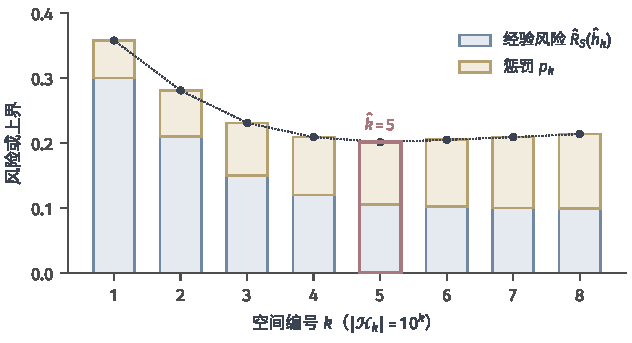
\includegraphics[width=107mm]{figures/06-foundations/02-learning-theory/matplotlib/lt7b-srm-penalty-selection/figure.pdf}
  \caption{SRM在八个嵌套有限空间之间的选择。每根柱子的下段（浅蓝）是该空间内最好假设的训练错误率，为教学取值；上段（浅黄）是按式~\eqref{eq:srm-finite-penalty}在$n=1000$、$\delta=0.05$、$\delta_k=\delta/[k(k+1)]$、$|\mathcal H_k|=10^k$下算出的惩罚$p_k$。点线连接两段之和，红框标出和最小的空间$\hat k=5$。}
  \label{fig:srm-penalty-selection}
\end{figure}

\paragraph{保证的含义与边界}

从式~\eqref{eq:srm-oracle}两侧减去贝叶斯风险，右边每一项变成“该空间的近似误差加$2p_k$”，再加求解容差$\rho$。这给出第~\ref{sec:statistical-model-selection}节偏差与复杂度权衡的一条充分路线：嵌套空间扩大时类内最低风险不增，惩罚则通常增大，SRM的输出至少与这两项之和最小的空间相当。$2p_k$是统计代价的上界，不是估计误差本身；嵌套空间的类内最低风险也不保证严格下降，定理不要求$p_k$随编号严格增加。

定理有三项不能省略的条件。第一，定理中的惩罚在看样本前确定。若改用经验Rademacher复杂度$\widehat{\mathfrak R}_S(\mathcal G_k)$构造数据依赖的惩罚，需要先按定理~\ref{thm:rademacher-risk-bound}的第二式对每个空间建立以$\delta_k$为预算的偏差事件，再对全部空间求并；把事后算出的某个数值直接代入固定惩罚的式~\eqref{eq:srm-classwise-confidence}，推理并不成立；按前一种做法建立事件后，同一证明照样成立。第二，结论是对固定分布的高概率保证；要得到分布无关的保证，惩罚必须对全部允许分布使用同一组上界。第三，定理只评价已经得到的输出，没有给出高效求解式~\eqref{eq:structural-risk-minimization}的程序。空间数可能无限、每个空间内的经验风险最小化也可能难以计算；这些计算问题只能作为求解容差$\rho$进入结论，不能被统计保证消去。

\subsection{集成学习}
\label{sec:boosting}
\label{sec:ensemble-learning-guarantees}

单个预测器可能对训练样本的扰动较敏感，或者表达不了所需的判定边界。把多个预测器的回答组合起来，称为\term{集成学习}（ensemble learning）。本小节不按方法逐一介绍，而是回答三个理论问题：组合以后候选集合的复杂度怎样计算，经验表现怎样连接到总体风险，弱学习在什么条件下能提升为强学习。

\subsubsection{集成预测与组合类}

常见的集成方法在两处有所不同：成员怎样产生，以及成员怎样组合。\term{装袋法}（bootstrap aggregating, bagging）在原样本的多份有放回重抽样上分别训练成员，再平均得分或投票\scite{breiman1996bagging}；\term{随机森林}（random forest）在此基础上还在每次分裂时随机选择候选特征，以得到彼此差别更大的决策树\scite{breiman2001randomforests}。\term{提升}（boosting）按顺序添加成员，每个新成员针对此前组合的不足来训练，梯度提升把这一过程写成函数空间中的逐步下降\scite{friedman2001gradientboost}。堆叠法（stacking）则把成员的输出当作新特征，再学习一个组合规则\scite{wolpert1992stacked}。这些方法的模型细节、训练步骤和实践要点属于模型卷，这里只用它们说明：成员可以由数据选出，组合规则既可以固定，也可以学习。

为统一分析，把集成预测器写成
\[
 f(x)=g\bigl(h_1(x),\ldots,h_M(x)\bigr),
\]
其中$h_m$取自成员类$\mathcal B$，组合规则$g$取自组合规则类$\mathcal C$，成员数$M$不超过事先给定的上限。由这三项共同规定的全部预测器组成组合类$\mathcal F$。常见的三种组合规则是：回归中的平均$g(u_1,\ldots,u_M)=M^{-1}\sum_mu_m$；二分类中的加权得分$\sum_ma_mu_m$；以及对得分取符号的\term{加权投票}（weighted voting），等权时为\term{多数投票}（majority voting）。

有两点必须在抽样前说清。其一，$\mathcal F$是事先规定的集合，成员与组合系数则可以看过样本后选出；后面的统一风险界控制的正是$\mathcal F$，才能覆盖这种数据依赖的选择。其二，同一个集成可以按两种对象评价：实值得分$f$配上平方损失、逻辑损失或间隔损失，以及最终分类器$\operatorname{sign}f$配上零一损失。两种对象的复杂度不同，不能把得分类的复杂度当作分类器类的复杂度，反之亦然。

\subsubsection{统一风险比较}

设损失可测且取值于$[0,1]$（或满足所用工具要求的尾部条件），记集成算法的输出为$\hat f\in\mathcal F$。定义组合类上的共同偏差与实际经验优化差
\[
 \Delta_S=\sup_{f\in\mathcal F}|R_{\mathcal P}(f)-\hat R_S(f)|,
 \qquad
 \rho_S=\hat R_S(\hat f)-\inf_{f\in\mathcal F}\hat R_S(f).
\]
在同一份样本上，输出一侧给出直接形式的界
\begin{equation}
 R_{\mathcal P}(\hat f)\leq\hat R_S(\hat f)+\Delta_S,
 \label{eq:ensemble-direct-risk}
\end{equation}
再按定理~\ref{thm:approximate-erm-risk}的三步比较，得到相对类内最优的界
\begin{equation}
 R_{\mathcal P}(\hat f)-\inf_{f\in\mathcal F}R_{\mathcal P}(f)\leq2\Delta_S+\rho_S.
 \label{eq:ensemble-excess-risk}
\end{equation}
两式对任何满足条件的集成构造都适用。它们不预设训练程序实现了经验最优：装袋法、提升和堆叠法都只是某种程序，实际达到的$\rho_S$要另外计算。本节余下部分的任务因此分成两项：用复杂度控制$\Delta_S$，用具体构造控制经验拟合。

数据依赖须与$\mathcal F$的规定相符。若成员与组合规则使用同一份样本，就要对完整的组合类控制$\Delta_S$，其中包含成员的选择。若组合规则在一份与成员训练独立的样本上学习，可以先条件于已经训练好的成员，此时只需控制组合规则类，成员被当作固定特征。堆叠法常用的折外预测、事后挑选成员和最终在全部样本上重训，各自改变了哪些量依赖哪份数据，须逐项核对。装袋法的袋外误差在每个观测上只用没有抽到它的那部分成员评价，不同观测对应不同的子集成；它也就不是最终集成的同一个经验风险，不能直接代入式~\eqref{eq:ensemble-direct-risk}。

比较基准也要说清。若$\mathcal F$包含“只用一个成员”的组合（例如权重可以全部放在一个成员上），式~\eqref{eq:ensemble-excess-risk}的右侧就不劣于最佳单个成员；否则这个比较没有依据。平均为什么可能有益，可以在凸损失下看清。设预测空间对平均封闭、损失关于预测凸，$\bar f=M^{-1}\sum_mf_m$。由Jensen不等式，逐点有$\ell(\bar f(x),y)\leq M^{-1}\sum_m\ell(f_m(x),y)$，取期望得
\[
 R_{\mathcal P}(\bar f)\leq\frac1M\sum_{m=1}^MR_{\mathcal P}(f_m).
\]
平方损失下还有精确等式$R(\bar f)=M^{-1}\sum_mR(f_m)-\mathbb E[M^{-1}\sum_m(f_m(x)-\bar f(x))^2]$：成员间预测分歧越大，平均成员风险被扣减得越多。但这只与成员平均比较，不与最佳成员比较。两个成员在某输入处分别比真值高0.1和高0.5，平方误差为0.01和0.25，平均预测高0.3，误差0.09，低于成员平均0.13，却高于最佳成员的0.01。

装袋法降低的是训练随机性造成的预测波动。在固定输入$x$处，把各成员得分$F_m(x)$看作训练样本与重抽样的随机函数，设方差都为$v$、两两协方差都为$c$，平均得分的方差为
\[
 \operatorname{Var}\left(\frac1M\sum_{m=1}^MF_m(x)\right)=\frac vM+\frac{M-1}Mc.
\]
取$v=0.04$、$c=0.01$、$M=10$，方差为$0.004+0.009=0.013$；$M$再大也降不到$c=0.01$以下。各次重抽样都来自同一份原样本，成员一般相关，$c=0$是理想情形。方差下降也不直接等于零一风险下降：分类结果取决于得分是否越过0。

零一损失下，投票甚至可能劣于每个成员。把输入空间分成概率各为$1/6$的三块$A_1,A_2,A_3$，其余概率$1/2$的部分三个分类器都判对。令$h_1$在$A_1\cup A_2$上出错，$h_2$在$A_1\cup A_3$上出错，$h_3$在$A_2\cup A_3$上出错。每个成员的风险都是$1/3$，而在每一块上恰有两个成员出错，多数投票在$A_1\cup A_2\cup A_3$上全错，风险为$1/2$。投票能纠正的只是少数成员的错误；错误集中在同一批输入上时，投票不起作用。反过来，若给定$(x,y)$时各成员的错误关于训练随机性相互独立、每个成员的条件错误概率都不超过$1/2-\gamma$，$T$个成员（$T$为奇数）的多数投票出错要求错误比例达到$1/2$，Hoeffding不等式给出$\mathbb E_{\mathrm{train}}R_{\mathcal P}(H)\leq e^{-2T\gamma^2}$。这两个条件都很强，错误互不相关也不能代替独立性；它们只说明理想条件下投票为何有效。

\subsubsection{组合类的复杂度}

接下来控制式~\eqref{eq:ensemble-excess-risk}中的$\Delta_S$。先看二分类基规则$\mathcal B\subseteq\{-1,1\}^X$及固定成员数的加权投票。组合系数是实数，有无穷多种取法；关键是在有限输入上，它们只能产生有限多种预测。

\begin{theorem}[投票假设空间的生长函数]
\label{thm:vote-growth-infinite}
设$X$为非空集合，$\mathcal B\subseteq\{-1,1\}^X$非空。对整数$T\geq1$，令$\mathcal V_T$包含所有形如
\[
 x\mapsto\operatorname{sign}\!\left(\sum_{t=1}^T a_t h_t(x)\right),
 \qquad h_t\in\mathcal B,\quad a_1,\ldots,a_T\in\mathbb R,
\]
的投票分类器，并预先固定得分为0时的标签。对任意二分类函数空间$\mathcal F$，记$\Pi_{\mathcal F}(m)$为它在$m$个输入上能产生的预测向量个数的最大值。则对任意整数$m\geq T+1$，
\begin{equation}
 \Pi_{\mathcal V_T}(m)
 \leq\Pi_{\mathcal B}(m)^T
       \left(\frac{em}{T+1}\right)^{T+1}.
 \label{eq:boosting-vote-growth}
\end{equation}
若$d=\operatorname{VC}(\mathcal B)$满足$1\leq d<\infty$，则在$m\geq\max\{d,T+1\}$时，
\begin{equation}
 \log\Pi_{\mathcal V_T}(m)
 \leq dT\log\frac{em}{d}+(T+1)\log\frac{em}{T+1}.
 \label{eq:infinite-boosting-growth}
\end{equation}
特别地，对每个固定有限的$T$，$\mathcal V_T$的VC维有限。
\end{theorem}

\begin{proof}
固定$m$个输入。每个基规则在这些输入上至多产生$\Pi_{\mathcal B}(m)$种预测向量，$T$个基规则的预测排成$m\times T$的矩阵，因而至多有$\Pi_{\mathcal B}(m)^T$种矩阵。

固定一种矩阵后，把第$i$个输入表示为该矩阵的第$i$行，即$T$维向量$\bm u_i=(h_1(x_i),\ldots,h_T(x_i))$。改变权重$a$，就是在这$m$个$T$维点上改变一个过原点的线性分类器。它们包含于$\mathbb R^T$上仿射半空间类，后者VC维为$T+1$；Sauer--Shelah引理（引理~\ref{lem:sauer-shelah}）把这个矩阵上能产生的预测数控制为$(em/(T+1))^{T+1}$。对所有矩阵求和，即得第一式。

基类VC维为$d$时，代入$\Pi_{\mathcal B}(m)\leq(em/d)^d$并取对数，得到第二式。固定$d,T$后，上界关于$m$至多多项式增长，不能对任意大的$m$达到$2^m$，所以投票类的VC维有限。$d=0$时基类在各点的预测唯一，由第一式可作同样判断。
\end{proof}

以实数轴上的阈值规则为例：$\mathcal B$包含$x\mapsto s\operatorname{sign}(x-\theta)$，$s\in\{-1,1\}$，取向与阈值都可选，VC维$d=2$。在$m$个不同输入上，阈值只能落在$m+1$个间隙中，再乘两种取向并去掉重复，至多$2m$种预测。取$T=10$、$m=1000$，式~\eqref{eq:boosting-vote-growth}给出$\log\Pi_{\mathcal V_{10}}(1000)\leq10\log2000+11\log(1000e/11)\approx137$，而全部标签模式的对数为$1000\log2\approx693$。基类无限并不妨碍分析，起作用的是基类在有限输入上的预测数。把这一生长函数代入第~\ref{sec:binary-learnability-characterization}节的VC一致收敛界（定理~\ref{thm:vc-uniform-convergence}），就得到$\mathcal V_T$上的$\Delta_S$，它随$T\log m$与$d T\log m$增长：成员数与基类容量都进入统一风险界。

对实值得分可以换一种算法。设$\mathcal B$为取值于$[-1,1]$的基函数类，它的\term{凸包}（convex hull）$\operatorname{conv}(\mathcal B)$由有限个基函数的非负、和为1的加权组合组成；凸包的成员是实值得分，取符号后才是分类器。凸包引理（引理~\ref{lem:rademacher-convex-hull}）说：固定输入样本后，$\widehat{\mathfrak R}_{S_X}(\operatorname{conv}(\mathcal B))=\widehat{\mathfrak R}_{S_X}(\mathcal B)$。原因是固定随机符号后，$n^{-1}\sum_i\sigma_if(x_i)$关于$f$是线性的，线性函数在凸包上的上确界等于在原集合上的上确界。这个等式不含成员数，因此对任意多个成员的归一化组合都成立。若$\mathcal B\subseteq\{-1,1\}^X$的VC维为$d$且$1\leq d\leq n$，基函数在样本上至多产生$\Pi_{\mathcal B}(n)$个预测向量，每个的欧氏范数为$\sqrt n$，Massart引理与Sauer--Shelah引理给出
\begin{equation}
 \widehat{\mathfrak R}_{S_X}(\mathcal B)
 \leq\sqrt{\frac{2\log\Pi_{\mathcal B}(n)}{n}}
 \leq\sqrt{\frac{2d\log(en/d)}{n}}.
 \label{eq:ensemble-base-rademacher}
\end{equation}

两种算法控制的对象不同。VC计数控制取符号后的投票分类器，代价随$T$增长；凸包等式控制归一化得分，代价不含$T$。凸包结论不能直接用于零一损失，因为零一损失关于得分不连续，收缩引理不适用；下一小节用间隔损失把二者连接起来。

推广到其他组合方式时，需要控制的量随之改变。带符号的加性组合$\sum_ma_mh_m$可写成$\|a\|_1$乘以$\mathcal B\cup(-\mathcal B)$的凸包中的元素，复杂度按系数绝对值总量$\|a\|_1$线性放大，因此要约束$\|a\|_1$而不是成员数。学习非线性组合规则（如堆叠法中的神经网络）时，还要控制成员与组合规则形成的复合类。成员数、系数大小和组合规则的灵活性都可能扩大可选函数的集合，仅凭“这是模型平均”不能断定复杂度下降。

\subsubsection{分类间隔与泛化保证}

按成员数计算复杂度可能过于保守：许多成员的权重可能很小，组合得分也可能离判定边界很远，这些信息都没有被利用。沿用标签$y\in\{-1,1\}$，对非负、和为1的权重$a_m$，令$f=\sum_ma_mh_m\in\operatorname{conv}(\mathcal B)$。乘积$yf(x)$称为归一化得分的分类\term{间隔}（margin）：成员取值于$\{-1,1\}$时，它等于投对一侧的总权重减去投错一侧的总权重。投对一侧占0.9时，间隔为$0.9-0.1=0.8$；只占0.51时，间隔为0.02。两种情况下预测都正确，但后者只要改变少量权重就会出错。正数比例缩放不改变$\operatorname{sign}f$，归一化把得分放到$[-1,1]$这一共同尺度上，间隔的大小因此可以比较。训练样本上全部间隔的经验分布称为\term{间隔分布}（margin distribution）。

在抽样前固定$\rho>0$，取第~\ref{sec:rademacher-complexity}节的间隔损失$\ell_\rho$：间隔不大于0时为1，在$(0,\rho)$内线性下降，不小于$\rho$时为0。它处处不小于零一损失，关于得分为$1/\rho$-Lipschitz，并且在训练样本上不超过小间隔示性$\mathbb I\{y_if(x_i)\leq\rho\}$。

\begin{theorem}[集成的间隔风险界]
\label{thm:ensemble-margin-risk}
\label{thm:learning-ensemble-convex-hull}
设$(X,\mathcal X)$为可测空间，$Y=\{-1,1\}$，$\mathcal P$为$X\times Y$上的概率分布，$S=((x_i,y_i))_{i=1}^n\sim\mathcal P^n$，$S_X=(x_1,\ldots,x_n)$。设$\mathcal B$为抽样前固定的非空可测函数类，取值于$[-1,1]$，并满足定理~\ref{thm:rademacher-risk-bound}所需的可数逼近条件（对相应的间隔损失类）。事先固定$\rho>0$与$\delta\in(0,1)$。则以至少$1-\delta$的概率，所有$f\in\operatorname{conv}(\mathcal B)$同时满足
\begin{equation}
 \mathbb P_{(x,y)\sim\mathcal P}\{yf(x)\leq0\}
 \leq\frac1n\sum_{i=1}^n\mathbb I\{y_if(x_i)\leq\rho\}
 +\frac{2}{\rho}\widehat{\mathfrak R}_{S_X}(\mathcal B)
 +3\sqrt{\frac{\log(2/\delta)}{2n}}.
 \label{eq:ensemble-margin-bound}
\end{equation}
左侧把零得分也计为错误，因此上界任意固定平局规则下$\operatorname{sign}f$的零一风险。
\end{theorem}

\begin{proof}
令$\mathcal G=\{(x,y)\mapsto\ell_\rho(yf(x)):f\in\operatorname{conv}(\mathcal B)\}$，它取值于$[0,1]$。对$\mathcal G$应用定理~\ref{thm:rademacher-risk-bound}的经验复杂度版本：以至少$1-\delta$的概率，所有$f$同时满足
\[
 \mathbb E\,\ell_\rho(yf(x))
 \leq\frac1n\sum_i\ell_\rho(y_if(x_i))+2\widehat{\mathfrak R}_S(\mathcal G)
 +3\sqrt{\frac{\log(2/\delta)}{2n}}.
\]
左侧不小于$\mathbb P\{yf(x)\leq0\}$，因为间隔损失在非正间隔处为1；右侧第一项不超过小间隔比例，因为间隔损失在间隔不小于$\rho$时为0、在其余位置不超过1。

剩下计算$\widehat{\mathfrak R}_S(\mathcal G)$。对每个$i$，$u\mapsto\ell_\rho(y_iu)$是$1/\rho$-Lipschitz的标量函数，收缩引理（引理~\ref{lem:rademacher-contraction}）给出$\widehat{\mathfrak R}_S(\mathcal G)\leq\rho^{-1}\widehat{\mathfrak R}_{S_X}(\operatorname{conv}(\mathcal B))$。这里用到收缩引理允许逐观测使用不同的Lipschitz函数，标签$y_i$正是通过这种方式进入。最后由凸包引理（引理~\ref{lem:rademacher-convex-hull}），凸包的经验复杂度等于$\mathcal B$的经验复杂度。三步合并即得式~\eqref{eq:ensemble-margin-bound}。
\end{proof}

这是总体零一风险的直接上界，对应式~\eqref{eq:ensemble-direct-risk}：右侧由经验小间隔比例与复杂度代价组成，不是相对某个基准的超额风险。若要与类内最优比较，还须另行控制参照一侧的偏差，并处理间隔损失与零一损失的差别。

\paragraph{数值与间隔阈值}

以前面的阈值基类为例，$d=2$。取$n=10^5$，由式~\eqref{eq:ensemble-base-rademacher}，$\widehat{\mathfrak R}_{S_X}(\mathcal B)\leq\sqrt{2\log(2\times10^5)/10^5}\approx0.0156$。$\rho=0.2$时复杂度项约为$2\times0.0156/0.2\approx0.156$，$\delta=0.05$时末项约为$3\sqrt{\log40/(2\times10^5)}\approx0.013$，合计约0.169。若训练样本上没有间隔不大于0.2的观测，零一风险至多约0.17。同一阈值若取$n=10^4$、$\rho=0.1$，复杂度项约为0.89，界几乎没有信息。这说明界的价值同时取决于样本量与实际达到的间隔。

间隔阈值必须事先固定。若想看过间隔分布再选$\rho$，可以在网格$\rho_j=2^{-j}$（$j=1,2,\ldots$）上分配预算$\delta_j=\delta/[j(j+1)]$，对每个$j$应用定理再求并集，这正是第~\ref{sec:srm}节的失败预算：选中的$\rho_j$只需把$\log(2/\delta)$换成$\log(2j(j+1)/\delta)$，代价只按$\log j$增长。

式~\eqref{eq:ensemble-margin-bound}不显含成员数，与定理~\ref{thm:vote-growth-infinite}的计数界形成对照：后者随$T$增长，前者只依赖基类复杂度、实际间隔和阈值。这为一个经验现象提供了一种解释：提升的轮数继续增加、训练错误已经为零时，测试错误不一定上升\scite{schapire1998margin}。但界并不保证间隔一定随成员数增加而增大，也不能推出成员越多泛化越好；它只说明，在训练间隔变大的情形下，风险上界可以不随成员数恶化。

\subsubsection{从弱学习到强学习}

前三小节控制了统计偏差，但没有说明怎样得到训练间隔大或训练错误小的组合。提升回答的正是这一问题：只要有一个比随机猜测略好、而且在所有需要的分布上都略好的学习器，就能把训练错误压到任意小。

\paragraph{统一的弱优势}

第~\ref{sec:pac-learning}节定义了\term{弱学习}（weak learning）：存在$\gamma\in(0,1/2)$、同一个算法$A$与有限的样本量函数，使对每个可实现分布，$A$都以高概率输出风险至多$1/2-\gamma$的假设。与之相对，能达到任意精度的学习称为\term{强学习}（strong learning）。弱学习的关键在量词顺序：优势$\gamma$和算法$A$先于分布确定，对每个可实现分布都要成立。提升会对训练样本重新加权，每一轮制造一个新的经验分布；这些分布仍然可实现（重加权只改概率，不改标签），所以弱学习器在每一轮都能保持同样的优势。只在原始分布上略好于猜测是不够的，优势可以很小，但不能在权重改变之后消失。本小节要证明：在可实现二分类中，若基类VC维有限且存在这样的弱学习器，就能构造PAC学习器。这一结论最早由Schapire证明\scite{schapire1990strength}，下面采用AdaBoost的构造\scite{freund1997boosting}。

\paragraph{AdaBoost的训练错误}

AdaBoost只需要下面几项。用$D^{(t)}$表示第$t$轮训练样本上的权重，各分量非负、和为1，初始$D^{(1)}(i)=1/n$。得到基分类器$h_t$后，计算加权错误率$e^{(t)}=\sum_iD^{(t)}(i)\mathbb I\{h_t(x_i)\neq y_i\}$，令投票系数$\alpha^{(t)}=\frac12\log\frac{1-e^{(t)}}{e^{(t)}}$，把分对样本的权重乘以$e^{-\alpha^{(t)}}$、分错样本的权重乘以$e^{\alpha^{(t)}}$，再归一化。$e^{(t)}<1/2$时$\alpha^{(t)}>0$，分错样本的相对权重上升；下一轮要使加权错误率低于$1/2$，就必须更多地判对这些样本。$e^{(t)}=0$时$h_t$与全部样本一致，直接输出并停止。

为什么投票系数取这个值？把归一化常数写成$\alpha$的函数，分对与分错两组分别贡献$(1-e)e^{-\alpha}$与$ee^{\alpha}$：
\[
 Z(\alpha)=(1-e)e^{-\alpha}+ee^{\alpha}.
\]
令导数为零，得$e^{2\alpha}=(1-e)/e$，即上面的$\alpha^{(t)}$；代回得$Z=2\sqrt{e(1-e)}$。下一定理说明，训练错误不超过各轮$Z^{(t)}$之积，所以这个系数正是逐轮最小化训练错误上界的选择。代入后，被分错样本的总权重从$e$变为$e\sqrt{(1-e)/e}/Z=1/2$：刚用过的$h_t$在新权重下的错误率恰为$1/2$，不能再提供优势，下一轮必须换一个规则。

\begin{theorem}[AdaBoost经验风险界]
\label{thm:adaboost-training}
\label{thm:adaboost-training-error}
设$T,n\geq1$，$S=((x_i,y_i))_{i=1}^n$且$y_i\in\{-1,1\}$。AdaBoost初始化$D^{(1)}(i)=1/n$；第$t$轮取得$h_t:X\to\{-1,1\}$后计算
\[
 e^{(t)}=\sum_{i=1}^nD^{(t)}(i)\mathbb I\{h_t(x_i)\neq y_i\}.
\]
若每轮均有$0<e^{(t)}<1/2$，令
\[
 \alpha^{(t)}=\frac12\log\frac{1-e^{(t)}}{e^{(t)}},\qquad
 Z^{(t)}=\sum_{i=1}^nD^{(t)}(i)e^{-\alpha^{(t)}y_i h_t(x_i)},
\]
\[
 D^{(t+1)}(i)
 =\frac{D^{(t)}(i)e^{-\alpha^{(t)}y_i h_t(x_i)}}{Z^{(t)}},
 \qquad
 H_T(x)=\operatorname{sign}\!\left(\sum_{t=1}^T\alpha^{(t)}h_t(x)\right),
\]
其中得分为0时采用预先固定的平局规则。记$\gamma^{(t)}=1/2-e^{(t)}$，并以零一损失定义$\hat R_S(H_T)=n^{-1}\sum_i\mathbb I\{H_T(x_i)\neq y_i\}$，则
\begin{equation}
 \hat R_S(H_T)\leq\prod_{t=1}^T Z^{(t)}
 =\prod_{t=1}^T2\sqrt{e^{(t)}(1-e^{(t)})}
 \leq\exp\left(-2\sum_{t=1}^T(\gamma^{(t)})^2\right).
 \label{eq:adaboost-training-bound}
\end{equation}
若每轮$\gamma^{(t)}\geq\gamma>0$，右端不超过$e^{-2T\gamma^2}$。
\end{theorem}

\begin{proof}
记$F_T(x)=\sum_{t=1}^T\alpha^{(t)}h_t(x)$。把权重递推从第1轮展开到第$T$轮，指数中的各项相加，得到
\[
 D^{(T+1)}(i)=\frac{\exp(-y_iF_T(x_i))}{n\prod_{t=1}^TZ^{(t)}}.
\]
若样本$i$被$H_T$分错，则$y_iF_T(x_i)\leq0$（得分为0时无论平局规则如何都满足），于是$\mathbb I\{H_T(x_i)\neq y_i\}\leq\exp(-y_iF_T(x_i))$。对$i$求平均并代入上式，
\[
 \hat R_S(H_T)\leq\frac1n\sum_i\exp(-y_iF_T(x_i))
 =\prod_{t=1}^TZ^{(t)}\sum_iD^{(T+1)}(i)=\prod_{t=1}^TZ^{(t)},
\]
最后一步用了新权重之和为1。第一个等式由前面的计算$Z^{(t)}=2\sqrt{e^{(t)}(1-e^{(t)})}$得到。代入$e^{(t)}=1/2-\gamma^{(t)}$，有$2\sqrt{e(1-e)}=\sqrt{1-4(\gamma^{(t)})^2}$；再用$1-u\leq e^{-u}$并开方，得$\sqrt{1-4\gamma^2}\leq e^{-2\gamma^2}$。逐轮相乘即得末界。
\end{proof}

证明中的中间量$n^{-1}\sum_i\exp(-y_iF_T(x_i))$是指数代理损失下的训练风险。它是零一训练错误的上界，每轮按因子$Z^{(t)}<1$严格下降；零一训练错误本身则不保证每轮都下降。

图~\ref{fig:adaboost-weights-training}在一个十点教学样本上运行这一构造。输入为$x_i=i$，标签依次为$(+,+,+,-,+,+,-,-,+,-)$，基类为两种取向的全部阈值规则，每轮精确求加权错误率最小的阈值。第1轮的阈值放在6.5（右侧判负），$e^{(1)}=0.2$，分错的是$x_4$与$x_9$；更新后这两个样本的权重各升到0.25，其余八个各降到0.0625。此后的轮次里，权重始终集中在$x_4$与$x_9$上，其次是$x_7,x_8$：它们与相邻样本标签相反，单个阈值很难同时判对它们与邻居。右图中，$\prod_tZ^{(t)}$与$e^{-2\sum(\gamma^{(t)})^2}$都按指数下降，$T=10$时分别约为0.377和0.422。训练错误率在第8轮首次为0，第9轮回到0.1，从第10轮起保持为0，这正是零一训练错误不单调的一个实例。由于十个样本的训练错误只能取$0,0.1,\ldots$，乘积界在第26轮降到0.1以下以后，就保证训练错误为0。

\begin{figure*}[htbp]
  \centering
  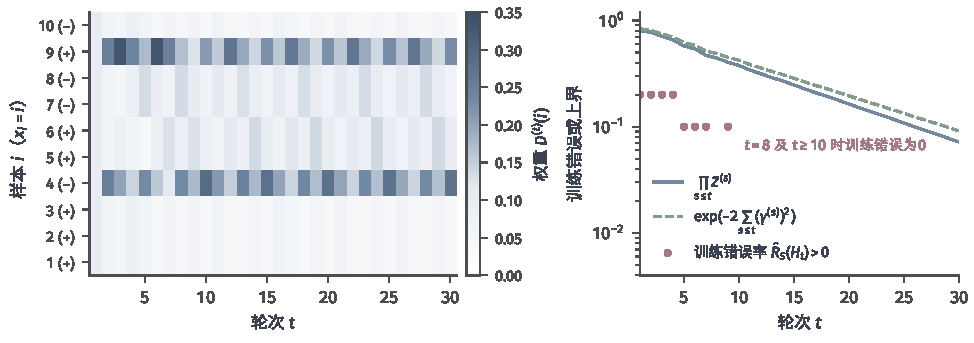
\includegraphics[width=165mm]{figures/06-foundations/02-learning-theory/matplotlib/lt7b-adaboost-weights-training/figure.pdf}
  \caption{AdaBoost在十点教学样本上的权重与训练错误。样本为$x_i=i$，括号内为标签，基类为两种取向的阈值规则，每轮取加权错误率最小者。左：第$t$轮开始时的权重$D^{(t)}(i)$，颜色越深权重越大；权重很快集中到与邻居标签相反的样本4和9。右：对数纵轴上的乘积界$\prod_{s\leq t}Z^{(s)}$（实线）与指数界（虚线），圆点为非零的训练错误率；训练错误在$t=8$与$t\geq10$时为0。}
  \label{fig:adaboost-weights-training}
\end{figure*}

同一次运行的间隔分布见图~\ref{fig:ensemble-margin-distribution}。归一化得分$f_T=\sum_t\alpha^{(t)}h_t/\sum_s\alpha^{(s)}$的最小间隔在$T=1,5,10,30,200$时分别为$-1$、$-0.283$、0.049、0.156与0.193。训练错误为零以后，最小间隔仍在增大；与此同时，原来间隔很大的样本（$T=5$时有四个间隔为0.632）的间隔下降到约0.21，整个分布向一个较窄的区间收拢。按式~\eqref{eq:ensemble-margin-bound}，起作用的是小间隔比例，所以这种变化有利于风险上界，即使训练错误已不再下降。

\begin{figure}[htbp]
  \centering
  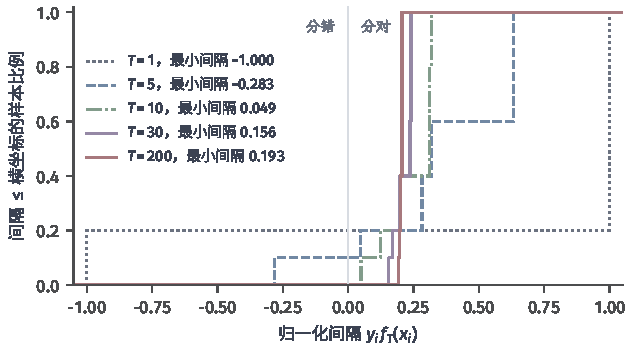
\includegraphics[width=107mm]{figures/06-foundations/02-learning-theory/matplotlib/lt7b-ensemble-margin-distribution/figure.pdf}
  \caption{图~\ref{fig:adaboost-weights-training}同一次运行的间隔分布。横轴为归一化间隔$y_if_T(x_i)$，纵轴为间隔不超过横坐标的样本比例，五条阶梯线对应$T=1,5,10,30,200$。曲线向右移动表示小间隔样本减少；图例给出各轮的最小间隔。}
  \label{fig:ensemble-margin-distribution}
\end{figure}

\paragraph{PAC提升}

训练界只控制经验风险。要把它变成总体风险的保证，还需让投票类的复杂度受控。顺序很关键：先由目标精度确定轮数$T$，再按$\mathcal V_T$的复杂度确定原样本量。

\begin{theorem}[有限VC维基假设空间下的弱学习提升]
\label{thm:pac-boosting}
\label{thm:finite-class-boosting}
\label{thm:finite-vc-boosting}
设$(X,\mathcal X)$为可测空间，$Y=\{-1,1\}$，目标假设空间$\mathcal H\subseteq Y^X$与固定基假设空间$\mathcal B\subseteq Y^X$均由可测分类器组成且非空，并采用零一损失$R_{\mathcal Q}(h)=\mathbb P_{(x,y)\sim\mathcal Q}\{h(x)\neq y\}$。假定$\operatorname{VC}(\mathcal B)<\infty$，允许$|\mathcal B|=\infty$；对每个固定整数$T\geq1$，由$T$个基假设和任意实权重形成、采用固定平局规则的投票空间，其零一损失函数均可测，并存在可数损失子类，使每个投票损失函数都是该子类中某个函数序列的逐点极限。假设存在同一个弱学习器$A$、固定的$\gamma\in(0,1/2)$和样本量函数$m_{\mathrm{weak}}:(0,1)\to\mathbb N$，使得对每个$\mathcal H$可实现分布$\mathcal Q$、每个$\eta\in(0,1)$及每个$m\geq m_{\mathrm{weak}}(\eta)$，用$S_{\mathrm{weak}}\sim\mathcal Q^m$训练$A$时，以至少$1-\eta$的概率输出$h\in\mathcal B$，且$R_{\mathcal Q}(h)\leq1/2-\gamma$；概率同时包含样本抽取和$A$的内部随机性。

对任意$\varepsilon,\delta\in(0,1)$，令$T=\lceil\log(2/\varepsilon)/(2\gamma^2)\rceil$。从$\mathcal H$可实现分布$\mathcal P$抽取原样本$S\sim\mathcal P^n$，初始化$D^{(1)}(i)=1/n$；第$t$轮从$D^{(t)}$给出的加权经验分布独立抽取$m_{\mathrm{weak}}(\delta/(2T))$个观测并调用$A$。若所得$h_t$的加权错误率为0，直接输出$h_t$；若错误率在$(0,1/2)$内，则按定理~\ref{thm:adaboost-training}取$\alpha^{(t)}$并更新权重；不满足这两种情况时按固定规则输出。完成$T$轮后输出$\operatorname{sign}(\sum_{t=1}^T\alpha^{(t)}h_t)$。则存在不依赖$\mathcal P$的$n_0(\varepsilon,\delta)$，使每个$n\geq n_0$时，该构造以至少$1-\delta$的概率输出零一风险不超过$\varepsilon$的分类器。概率同时来自原样本、各轮重新抽样及$A$的内部随机性；输出允许不属于$\mathcal H$。
\end{theorem}

\begin{proof}
给定$\varepsilon,\delta$，先于原样本固定$T$。定理~\ref{thm:vote-growth-infinite}保证$\mathcal V_T$的VC维有限；结合可数逼近条件，定理~\ref{thm:vc-uniform-convergence}给出不依赖$\mathcal P$的$n_0$，使$n\geq n_0$时，共同偏差事件
\[
 \sup_{H\in\mathcal V_T}|R_{\mathcal P}(H)-\hat R_S(H)|\leq\varepsilon/2
\]
的概率至少为$1-\delta/2$。

再看弱学习。原样本几乎必然由某个$h\in\mathcal H$实现，重加权只改变概率、不改变标签，所以每一轮的加权经验分布都是$\mathcal H$可实现的。条件于原样本及此前各轮的结果，独立重抽$m_{\mathrm{weak}}(\delta/(2T))$条观测再调用$A$，以至少$1-\delta/(2T)$的条件概率得到加权风险至多$1/2-\gamma$的$h_t$。对至多$T$轮使用并集界，全部实际调用的轮次都取得优势的概率至少为$1-\delta/2$。

两个成功事件同时发生时，若没有提前停止，定理~\ref{thm:adaboost-training}给出经验风险至多$e^{-2T\gamma^2}\leq\varepsilon/2$，这正是$T$的取法；若提前找到零加权错误的基假设，它的经验风险为0，且把其余权重取为零也属于$\mathcal V_T$。两种情况下输出都在$\mathcal V_T$中，偏差事件再给出总体风险至多$\varepsilon/2+\varepsilon/2=\varepsilon$。两类失败预算相加至多$\delta$，于是得到PAC保证。
\end{proof}

证明中三项预算各有来源：轮数$T$由训练界的指数速率与精度$\varepsilon/2$决定；原样本量由$\mathcal V_T$的复杂度与偏差$\varepsilon/2$决定；每轮的弱学习样本量由失败预算$\delta/(2T)$决定。证明没有假定各轮错误相互独立。它需要两个条件：基类VC维有限，以及弱学习器在全部可实现分布上具有统一优势。VC维有限并不保证弱学习器存在，优势条件要针对具体的$\mathcal H$另行证明\scite{shalevshwartz2014}。

条件不成立时，结论不能原样使用。若样本量固定而轮数不断增加，$\mathcal V_T$的复杂度随$T$增长，计数界失效，这时只能改用不含$T$的间隔界，并实际检查间隔。若基类VC维无限，两种界都要另找复杂度控制。若有标签噪声，重加权会把权重集中到噪声样本上，加权分布可能不再可实现，弱优势也可能消失，可实现情形的提升结论不能直接推广到不可知情形。这个构造说明的是弱到强的一种充分机制，不能代替装袋法、随机森林等其他集成方法各自的拟合条件。

\subsection{正则化}
\label{sec:regularized-learning}

第~\ref{sec:algorithmic-stability}节把学习保证分成两项：算法不能过度依赖个别训练观测，同时要在训练样本上取得接近最优的平均损失。那里的存在性构造（随机子采样再调用已知算法）只用于证明。实际使用的是正则化最小化一类算法，需要对它逐一算出稳定性代价和经验优化误差。本小节按三个问题展开：改写目标怎样影响解，怎样改善稳定性，又对原风险付出什么代价。

\subsubsection{凸学习}
\label{sec:convex-learning-problem}

零一损失关于参数是分段常数：参数的微小移动可能让损失从0跳到1，参数距离控制不住损失差；它的梯度几乎处处为零，也给不出改进方向。对线性分类器，真实标签为$+1$时，分数$\bm w^\top\bm x$从$-2$提高到$-0.1$，零一损失仍为1。训练中因此常换用\term{合页损失}（hinge loss）$\max\{0,1-y\bm w^\top\bm x\}$或逻辑损失$\log(1+e^{-y\bm w^\top\bm x})$。在上述例子中，合页损失从3降到1.1，分数达到1后才降为0，它还要求正确分类具有一定间隔。逻辑损失处处可微，合页损失在拐点处不可微：二者都能用于后面的凸正则化分析，却不能不加区分地套用要求光滑性的梯度定理。

这个例子提示了凸学习的两个要求：任意两个允许的决策之间作线性插值，仍是允许的决策；插值点的损失不超过两端损失的相应加权平均。下面用实赋范线性空间$(V,\|\cdot\|)$描述决策，取$\mathcal W\subseteq V$。凸性只依赖线性结构；Lipschitz常数与强凸常数还依赖所选范数，比较这些常数时必须使用同一范数。

\begin{definition}[凸学习问题]
\label{def:convex-learning-problem}
若$\mathcal W$是凸集，并且对每个$z\in Z$，函数$w\mapsto\ell(w,z)$为凸函数，则称该一般学习问题为凸学习问题。也就是说，对任意$u,v\in\mathcal W$、$t\in[0,1]$和$z\in Z$，有
\[
 \ell(tu+(1-t)v,z)\leq t\ell(u,z)+(1-t)\ell(v,z).
\]
\end{definition}

两种替代损失都可以按定义核对。合页损失是关于$\bm w$的两个仿射函数$0$与$1-y\bm w^\top\bm x$的逐点最大值，凸函数的逐点最大值仍凸；逻辑损失是$s\mapsto\log(1+e^{-s})$与线性函数$s=y\bm w^\top\bm x$的复合，前者的二阶导数$e^{-s}/(1+e^{-s})^2>0$，复合线性映射保持凸性。对固定样本，各条损失的平均仍凸，所以经验风险也凸。凸性针对训练中真正优化的变量：损失关于预测分数凸，并不保证把分数写成神经网络后关于网络参数仍凸。

凸性没有限制参数移动一点时损失能变化多少。后面要先估计相邻样本上两个解的距离，再把距离换算成损失差，所以还需要Lipschitz条件。

\begin{definition}[Lipschitz损失]
\label{def:lipschitz-loss}
若对任意$w,w'\in\mathcal W$与$z\in Z$都满足
\begin{equation}
 |\ell(w,z)-\ell(w',z)|\leq L\|w-w'\|,
 \label{eq:lipschitz-loss}
\end{equation}
则称损失关于该范数是$L$-Lipschitz的。
\end{definition}

常数$L=2$时，参数移动0.01，同一观测上的损失至多变化0.02。这里比较的是损失值；梯度分析中的光滑性比较的是梯度，两项条件不能混为一谈。凸问题也可以继续走一致收敛路线：$\|\bm w\|_2\leq B$、$\|\bm x\|_2\leq r$且损失关于得分$L$-Lipschitz时，式~\eqref{eq:linear-rademacher-bound}与收缩引理给出损失类复杂度上界$LBr/\sqrt n$。下面的稳定性分析是另一条算法层面的路线，不是说凸问题只能这样分析。

改用替代损失也改变了训练要最小化的风险。要把替代风险的改进联系到分类错误率，还需要\term{分类校准}（classification calibration）：在不限制预测函数表达能力时，替代风险趋于最优能够带来零一风险趋于贝叶斯风险。校准考察固定输入时的标签选择。记$\eta(x)=\mathbb P(y=1\mid x)$，$\eta(x)=0.7$时预测正类的条件错误率为0.3、预测负类为0.7，校准要求条件替代风险的最优得分也取正号。凸性解决怎样优化替代目标，校准解决这个目标是否与分类评价相容。校准只针对不受限的函数空间；在受限的线性类中，替代最优解不一定是零一最优解，还要另查线性类的近似能力。分类校准也不同于第~\ref{sec:reliability-output-evaluation}节的概率校准：后者比较预测概率与事件频率，二者之间没有一般的相互蕴含关系。

\subsubsection{强凸正则化}

凸性保证没有坏的局部最优，却不保证最优解唯一，更不保证它随样本平稳变化。以绝对损失$\ell(w,z)=|w-z|$为例，取两条观测$z_1=0$、$z_2=1$，经验风险$F_S(w)=(|w|+|w-1|)/2$在整个区间$[0,1]$上都等于$1/2$，每个点都是经验最优解。若算法在并列者中取最左端，输出为0；把$z_1$换成1，相邻样本的经验风险$F_{S'}(w)=|w-1|$只在$w=1$处最小。两个目标只差一项，输出却移动了整个区间（图~\ref{fig:regularized-minimizer-shift}左）。

我们希望加入一个确定的惩罚项，使偏离最优位置会带来足够大的目标增量，从而限制这种移动。取$\lambda>0$与惩罚$\Omega$，定义正则化算法
\begin{equation}
 A(S)\in\argmin_{w\in\mathcal W}
 \left\{\hat R_S(w)+\lambda\Omega(w)\right\}.
 \label{eq:regularized-erm}
\end{equation}
仅仅添加惩罚并不保证稳定，所需的是整个目标强凸。若存在$\mu>0$，使目标$F$满足
\begin{equation}
 F(tu+(1-t)v)\leq tF(u)+(1-t)F(v)
 -\frac\mu2t(1-t)\|u-v\|^2
 \label{eq:strong-convexity}
\end{equation}
对所有可行$u,v$及$t\in[0,1]$成立，则称$F$为\term{$\mu$强凸}（$\mu$-strongly convex）。与凸性相比，右端多减去一个与$\|u-v\|^2$成正比的量，要求函数在两点之间不能过于平坦。$F(w)=\mu w^2/2$恰好取等号，常数函数凸而不强凸。若最小点$w_*$存在，取$u=w$、$v=w_*$，左侧不小于$F(w_*)$，整理得$t(F(w)-F(w_*))\geq\frac\mu2t(1-t)\|w-w_*\|^2$；两边除以$t$再令$t\to0$，得到二次增长
\begin{equation}
 F(w)-F(w_*)\geq\frac\mu2\|w-w_*\|^2.
 \label{eq:quadratic-growth}
\end{equation}
离最小点越远，目标值必定高出越多。

回到绝对损失的例子，加入$\frac\lambda2w^2$并取$\lambda=2$。$F_S(w)+w^2$在$[0,1]$上等于$1/2+w^2$，最小点为0；$F_{S'}(w)+w^2=|w-1|+w^2$在$w<1$处导数为$2w-1$，最小点为$1/2$，值为$3/4$。两个最小点的距离从1缩小到$1/2$（图~\ref{fig:regularized-minimizer-shift}右）。下面的定理给出这一缩小的一般上界$2L/(\lambda n)$；这里$L=1$、$n=2$，上界恰为$1/2$，例子取到了等号。

\begin{figure}[htbp]
  \centering
  % 强凸正则化限制相邻样本最优解的移动。
% 绝对损失 l(w,z)=|w-z|，样本 S=(0,1)、相邻样本 S'=(1,1)，n=2。
% 左：F_S(w)=(|w|+|w-1|)/2 在 [0,1] 上恒为 1/2，按最左并列规则取 w=0；
%     F_{S'}(w)=|w-1|，唯一最小点 w'=1。两解相距 1。
% 右：加 (lambda/2) w^2，lambda=2：F_S+w^2 最小点 0（值 1/2），
%     F_{S'}+w^2=|w-1|+w^2 最小点 1/2（值 3/4）。两解相距 1/2，
%     恰等于定理界 2L/(lambda n)=2/(2*2)=1/2（L=1）。
% 坐标：x=1mm,y=1mm；w 每单位 28 mm，目标值每单位 16 mm。
\begingroup
\begin{tikzpicture}[figure picture,x=1mm,y=1mm]
  \def\wx{28}\def\fy{16}
  % ---------- 左面板 ----------
  \begin{scope}
    \draw[-{Stealth[length=1.6mm]},FigureStroke,line width=.6pt] (-0.3*\wx,0)--(1.32*\wx,0) node[right]{$w$};
    \draw[-{Stealth[length=1.6mm]},FigureStroke,line width=.6pt] (-0.25*\wx,0)--(-0.25*\wx,2.05*\fy);
    \foreach \t in {0,1}{\draw[FigureMuted,line width=.4pt] (\t*\wx,0)--(\t*\wx,-1.2) node[below,figure note]{$\t$};}
    \draw[FigureMuted,line width=.4pt] (0.5*\wx,0)--(0.5*\wx,-1.2) node[below,figure note]{$1/2$};
    \begin{scope}
      \clip (-0.25*\wx,0) rectangle (1.3*\wx,2.0*\fy);
      \draw[FigureBlue,line width=1.1pt,samples at={-0.25,-0.125,0,0.25,0.5,0.75,1,1.125,1.25}]
        plot ({\x*\wx},{\fy*(abs(\x)+abs(\x-1))/2});
      \draw[FigureRed,line width=1.1pt,dashed,samples at={-0.25,-0.125,0,0.25,0.5,0.75,1,1.125,1.25}]
        plot ({\x*\wx},{\fy*abs(\x-1)});
    \end{scope}
    \draw[FigureBlue,line width=2.2pt,opacity=.35] (0,0.5*\fy)--(\wx,0.5*\fy);
    \fill[FigureBlue] (0,0.5*\fy) circle (1.1);
    \fill[FigureRed] (\wx,0) circle (1.1);
    \draw[{Stealth[length=1.4mm]}-{Stealth[length=1.4mm]},FigureInk,line width=.6pt] (0,-8)--(\wx,-8);
    \node[figure note,anchor=north] at (0.5*\wx,-9) {两解距离 $1$};
    \node[figure heading] at (0.5*\wx,2.2*\fy+2) {未正则化};
    \node[font=\figurefont\footnotesize,text=FigureBlue] at (-0.14*\wx,0.78*\fy) {$F_S$};
    \node[font=\figurefont\footnotesize,text=FigureRed] at (0.24*\wx,1.02*\fy) {$F_{S'}$};
    \node[figure note,text=FigureBlue,anchor=north] at (0.22*\wx,0.46*\fy) {并列最优};
  \end{scope}
  % ---------- 右面板 ----------
  \begin{scope}[xshift=56mm]
    \draw[-{Stealth[length=1.6mm]},FigureStroke,line width=.6pt] (-0.3*\wx,0)--(1.32*\wx,0) node[right]{$w$};
    \draw[-{Stealth[length=1.6mm]},FigureStroke,line width=.6pt] (-0.25*\wx,0)--(-0.25*\wx,2.05*\fy);
    \foreach \t in {0,1}{\draw[FigureMuted,line width=.4pt] (\t*\wx,0)--(\t*\wx,-1.2) node[below,figure note]{$\t$};}
    \draw[FigureMuted,line width=.4pt] (0.5*\wx,0)--(0.5*\wx,-1.2) node[below,figure note]{$1/2$};
    \begin{scope}
      \clip (-0.25*\wx,0) rectangle (1.3*\wx,2.0*\fy);
      \draw[FigureBlue,line width=1.1pt,samples at={-0.25,-0.2,...,-0.05,0,0.05,...,0.95,1,1.05,1.1,1.15,1.2,1.25}]
        plot ({\x*\wx},{\fy*((abs(\x)+abs(\x-1))/2+\x*\x)});
      \draw[FigureRed,line width=1.1pt,dashed,samples at={-0.25,-0.2,...,-0.05,0,0.05,...,0.95,1,1.05,1.1,1.15,1.2,1.25}]
        plot ({\x*\wx},{\fy*(abs(\x-1)+\x*\x)});
    \end{scope}
    \fill[FigureBlue] (0,0.5*\fy) circle (1.1);
    \fill[FigureRed] (0.5*\wx,0.75*\fy) circle (1.1);
    \draw[FigureMuted,line width=.4pt,dash pattern=on 1.5pt off 1.5pt] (0.5*\wx,0.75*\fy)--(0.5*\wx,0);
    \draw[{Stealth[length=1.4mm]}-{Stealth[length=1.4mm]},FigureInk,line width=.6pt] (0,-8)--(0.5*\wx,-8);
    \node[figure note,anchor=north] at (0.5*\wx,-9) {两解距离 $1/2=2L/(\lambda n)$};
    \node[figure heading] at (0.5*\wx,2.2*\fy+2) {加 $\tfrac{\lambda}{2}w^2$，$\lambda=2$};
    \node[font=\figurefont\footnotesize,text=FigureBlue,anchor=east] at (0.86*\wx,1.75*\fy) {$F_S+w^2$};
    \node[font=\figurefont\footnotesize,text=FigureRed,anchor=west] at (1.02*\wx,0.72*\fy) {$F_{S'}+w^2$};
  \end{scope}
\end{tikzpicture}
\endgroup

  \caption{强凸正则化限制相邻样本最优解的移动。绝对损失，$S=(0,1)$，相邻样本$S'=(1,1)$。左：经验风险$F_S$（蓝实线）在$[0,1]$上并列最优，按最左规则取0；$F_{S'}$（红虚线）在1处最小，两解相距1。右：都加上$w^2$（$\lambda=2$）后，两条曲线的最小点分别为0与$1/2$，距离缩为$1/2$，恰等于定理~\ref{thm:regularized-erm-stability}中的$2L/(\lambda n)$。}
  \label{fig:regularized-minimizer-shift}
\end{figure}

一般证明使用同一机制。设相邻样本的最优解为$w$和$w'$。先用第一个目标比较$w'$与它的最小点$w$，再用第二个目标比较$w$与它的最小点$w'$，两次比较都由式~\eqref{eq:quadratic-growth}给出距离平方的下界。把它们相加后，两份样本中相同的$n-1$项和相同的正则项抵消，只剩被替换观测的贡献。定理要求损失为$L$-Lipschitz、惩罚$\Omega$为1-强凸，于是整个正则目标为$\lambda$-强凸。

\begin{theorem}[强凸正则化的稳定性]
\label{thm:regularized-erm-stability}
设$(Z,\mathcal Z)$为可测观测空间，$\mathcal W$是实赋范线性空间$(V,\|\cdot\|)$中的非空凸Borel集，$\ell:\mathcal W\times Z\to\mathbb R$可测。对每个$z\in Z$，函数$\ell(\cdot,z)$在$\mathcal W$上凸，并且对任意$u,v\in\mathcal W$都有
\[
 |\ell(u,z)-\ell(v,z)|\leq L\|u-v\|.
\]
设$\Omega:\mathcal W\to\mathbb R$可测，且对任意$u,v\in\mathcal W$和$t\in[0,1]$都有
\[
 \Omega(tu+(1-t)v)
 \leq t\Omega(u)+(1-t)\Omega(v)-\frac12t(1-t)\|u-v\|^2.
\]
固定$n\geq1$与$\lambda>0$。对每份$s=(z_1,\ldots,z_n)\in Z^n$，定义
\[
 A(s)\in\argmin_{w\in\mathcal W}
 \left\{\frac1n\sum_{i=1}^n\ell(w,z_i)+\lambda\Omega(w)\right\},
\]
并假定该最小解存在且$A$可测。目标函数的强凸性使最小解唯一；对任意只相差一个观测的$s,s'\in Z^n$及任意$z\in Z$，
\[
 \|A(s)-A(s')\|\leq\frac{2L}{\lambda n},\qquad
 |\ell(A(s),z)-\ell(A(s'),z)|\leq\beta_n,
\]
其稳定性常数满足
\begin{equation}
 \beta_n\leq\frac{2L^2}{\lambda n}.
 \label{eq:regularized-stability-bound}
\end{equation}
\end{theorem}

\begin{proof}
记$w=A(S)$、$w'=A(S')$，相应正则目标为$F_S$与$F_{S'}$。两个目标使用不同观测，不能直接比较最小值；我们分别在每个目标内比较这两个参数。$w$是$F_S$的最小点，$w'$是$F_{S'}$的最小点，由$\lambda$-强凸性的二次增长，
\begin{equation*}
 F_S(w')-F_S(w)\geq\frac\lambda2\|w-w'\|^2,
 \quad
 F_{S'}(w)-F_{S'}(w')\geq\frac\lambda2\|w-w'\|^2.
\end{equation*}
设$S$与$S'$只在第$i$项不同，分别为$z_i$与$z_i'$。两式相加并按观测整理，相同的$n-1$个损失项和相同的正则项全部抵消，只剩
\[
 \frac1n\Bigl[\ell(w',z_i)-\ell(w,z_i)+\ell(w,z_i')-\ell(w',z_i')\Bigr]
 \geq\lambda\|w-w'\|^2.
\]
方括号内两组差各由Lipschitz性控制为$L\|w-w'\|$，于是$\lambda\|w-w'\|^2\leq2L\|w-w'\|/n$。左侧随距离平方增长，右侧只随距离线性增长，所以距离不能太大：两解相同时结论已成立，否则除以$\|w-w'\|$，得$\|w-w'\|\leq2L/(\lambda n)$。最后在任意测试观测$z$上再用一次Lipschitz条件：
\[
 |\ell(w,z)-\ell(w',z)|\leq L\|w-w'\|\leq\frac{2L^2}{\lambda n}.
\]
\end{proof}

这是均匀稳定性：上界对所有相邻样本和所有测试观测同时成立。在所需可积性下，定理~\ref{thm:stability-expected-generalization}给出同样大小的期望泛化差上界。以$L_2$正则的逻辑回归核对条件：设$\|\bm x\|_2\leq r$，逻辑损失关于$\bm w$的梯度为$-y\bm x/(1+e^{y\bm w^\top\bm x})$，范数不超过$r$，所以它是$r$-Lipschitz的凸损失；取$\Omega(\bm w)=\|\bm w\|_2^2/2$，稳定性常数至多$2r^2/(\lambda n)$。$r=1$、$\lambda=0.1$、$n=1000$时，上界为0.02。岭回归需要特别核对区域。$\Omega(w)=\|w\|_2^2/2$在欧氏或一般Hilbert范数下展开$\|tu+(1-t)v\|^2$恰好使强凸不等式取等号，所以是1-强凸的；换成其他范数的平方未必如此。平方损失在无界参数上没有全局Lipschitz常数；只有限制输入、标签和参数后，才能由残差的上界得到有限的$L$。

\paragraph{稳定性与正则化代价的折中}

稳定性只控制了泛化差，还没有说明输出接近原问题的最优风险。算法最小化的是$\hat R_S(w)+\lambda\Omega(w)$，我们评价的仍是$R_{\mathcal P}(w)$。正则化的作用与代价因此出现在两项中。在均值估计中这两项可以显式算出：对$z_i\in[0,1]$，最小化$\frac1{2n}\sum_i(w-z_i)^2+\frac\lambda2w^2$得$\hat w=\bar z/(1+\lambda)$，替换一项后至多移动$1/[n(1+\lambda)]$；增大$\lambda$减小了移动，但输出的期望变成$m/(1+\lambda)$，偏离总体均值$m$的量为$\lambda m/(1+\lambda)$。

\begin{theorem}[正则化学习的期望风险保证]
\label{thm:regularized-learning-risk}
在定理~\ref{thm:regularized-erm-stability}的条件下，进一步设$\Omega:\mathcal W\to[0,\infty)$。令$S=(z_1,\ldots,z_n)\sim\mathcal P^n$，其中$\mathcal P$为$Z$上的概率分布，$A$为相应的可测正则化算法，$R_{\mathcal P}(w)=\mathbb E_{z\sim\mathcal P}\ell(w,z)$、$\hat R_S(w)=n^{-1}\sum_i\ell(w,z_i)$。假定独立测试损失$\ell(A(S),z)$、训练损失$\ell(A(S),z_i)$以及每个固定$w\in\mathcal W$的$\ell(w,z)$均可积。则对任意固定$w\in\mathcal W$，
\begin{equation}
 \mathbb E_S R_{\mathcal P}(A(S))-R_{\mathcal P}(w)
 \leq\frac{2L^2}{\lambda n}+\lambda\Omega(w).
 \label{eq:regularization-excess-risk}
\end{equation}
若$\mathcal W=\{w:\|w\|\leq B\}$为Hilbert空间中以原点为中心、半径$B>0$的闭球，$\Omega(w)=\|w\|^2/2$，且$L>0$，取$\lambda=2L/(B\sqrt n)$可得
\[
 \mathbb E_S R_{\mathcal P}(A(S))-\inf_{w\in\mathcal W}R_{\mathcal P}(w)
 \leq\frac{2LB}{\sqrt n}.
\]
\end{theorem}

\begin{proof}
正则目标的最优性给出$\hat R_S(A(S))+\lambda\Omega(A(S))\leq\hat R_S(w)+\lambda\Omega(w)$。由于$\Omega(A(S))\geq0$，去掉左侧的正则项后仍有$\hat R_S(A(S))\leq\hat R_S(w)+\lambda\Omega(w)$。比较决策$w$在抽样前固定，所以$\mathbb E_S\hat R_S(w)=R_{\mathcal P}(w)$；输出依赖样本，要借助稳定性才能把它的经验风险换成期望风险，二者的期望差至多$2L^2/(\lambda n)$。这正是定理~\ref{thm:expected-risk-comparison}的两项：期望泛化差与相对比较决策的经验差。两步合并得第一式。

在半径$B$的闭球内，$\Omega(w)=\|w\|^2/2\leq B^2/2$。代入所给$\lambda$，两项上界各为$LB/\sqrt n$，且对每个比较决策相同。对$w$取下确界即得第二式，不要求下确界可达。
\end{proof}

式~\eqref{eq:regularization-excess-risk}的两项分别来自稳定性与目标改写。$\lambda$越大，目标强凸性越强，解越不随单条观测移动，但目标也越偏离原经验风险。在半径$B$的球内，上界$U_n(\lambda)=2L^2/(\lambda n)+\lambda B^2/2$；令两项相等解出$\lambda^*=2L/(B\sqrt n)$，此时上界为$2LB/\sqrt n$。图~\ref{fig:regularization-tradeoff}取$L=B=1$：$n=100$时$\lambda^*=0.2$、上界0.2；$n=1000$时$\lambda^*\approx0.063$；$n=10^4$时$\lambda^*=0.02$、上界0.02。样本越多，单条观测的影响本来就越小，所需的正则化随之按$1/\sqrt n$减弱。增大$\lambda$只是使前一项上界减小、后一项上界增大，并不说明实际风险一定随之上升或下降。由平均超额风险界，再用超额风险非负与Markov不等式，得到充分样本量$n\geq(2LB/(\varepsilon\delta))^2$；这里没有声称对$\delta$的依赖是最优的。

\begin{figure}[htbp]
  \centering
  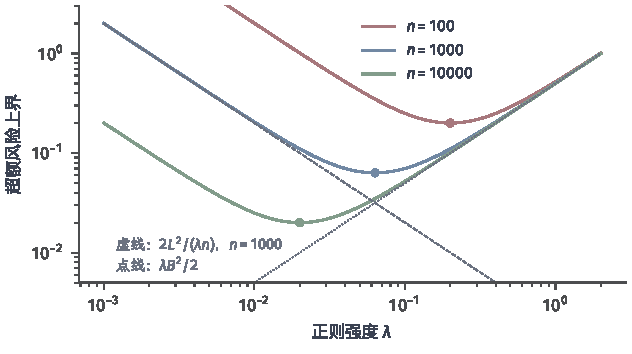
\includegraphics[width=107mm]{figures/06-foundations/02-learning-theory/matplotlib/lt7b-regularization-tradeoff/figure.pdf}
  \caption{正则强度的折中。三条实线是$L=B=1$时的上界$2L^2/(\lambda n)+\lambda B^2/2$，分别取$n=100,1000,10^4$，圆点为最小点$\lambda^*=2/\sqrt n$。灰色虚线与点线是$n=1000$时的两项：稳定性项随$\lambda$下降，比较项随$\lambda$上升且与$n$无关。双对数坐标下，$n$每增大十倍，最小点沿比较项直线左移半个数量级。}
  \label{fig:regularization-tradeoff}
\end{figure}

这个结论不显含参数维数，但依赖半径$B$与损失变化率$L$的统一控制。它与二分类的不可学习性结果并不矛盾：零一损失既不是凸损失，也不满足参数Lipschitz条件。以上还假定正则目标被精确最小化。若算法只返回近似解$\tilde A(S)$，满足$F_S(\tilde A(S))\leq\min F_S+\epsilon$，式~\eqref{eq:quadratic-growth}给出$\|\tilde A(S)-A(S)\|\leq\sqrt{2\epsilon/\lambda}$，相邻样本的两个近似解至多相距$2L/(\lambda n)+2\sqrt{2\epsilon/\lambda}$，经验比较也多出$\epsilon$。求解误差必须单独计入，目标强凸不能代替算法已经完成优化。

\subsubsection{弱凸正则化}
\label{sec:weakly-convex-regularization}

取消损失的凸性后，前面的相邻解比较还能用吗？以一维函数$-\kappa w^2/2$为例，加上$\lambda w^2/2$得$(\lambda-\kappa)w^2/2$，只有$\lambda>\kappa$时才强凸。一般地，若$\ell(\bm w,z)+\kappa\|\bm w\|_2^2/2$在凸决策集上为凸函数，就称损失是$\kappa$弱凸的（weakly convex），其中$\kappa\geq0$。在二阶可微的开凸域上，这等价于Hessian的全部特征值不小于$-\kappa$。弱凸参数度量损失最多有多大的负曲率；需要补偿的正是这部分负曲率。
% 保留旧位置锚点，不再重复编号定义。
\phantomsection\label{def:weakly-convex}

考虑模型$h_w(x)=w^2x$在观测$(x,y)=(1,1)$上的平方损失$(w^2-1)^2$。$w=\pm1$时损失为0，$w=0$时梯度也为0，损失却为1。它的二阶导数$12w^2-4\geq-4$，所以是4-弱凸的。若每条观测的损失都满足同一个弱凸上界$\kappa$，它们的平均也满足；加入强度$\lambda>\kappa$的二次正则项后，整个目标是$(\lambda-\kappa)$-强凸的。再保留Lipschitz条件，就能复用定理~\ref{thm:regularized-erm-stability}的相邻解比较。这里恢复的是修改后目标所确定的最优解的稳定性，原问题并没有因此变成凸问题。

\begin{theorem}[弱凸损失的正则化稳定性]
\label{thm:weakly-convex-regularization}
设$(Z,\mathcal Z)$为可测观测空间，$\mathcal W=\{\bm w\in\mathbb R^d:\|\bm w\|_2\leq B\}$，其中$B\geq0$，并设$\ell:\mathcal W\times Z\to\mathbb R$可测。固定$\kappa\geq0$和$L\geq0$；对每个$z\in Z$，函数$\bm w\mapsto\ell(\bm w,z)+\kappa\|\bm w\|_2^2/2$在$\mathcal W$上凸，且
\[
 |\ell(\bm u,z)-\ell(\bm v,z)|\leq L\|\bm u-\bm v\|_2
 \quad\text{对任意 }\bm u,\bm v\in\mathcal W.
\]
固定$n\geq1$并取$\lambda>\kappa$。对$S=(z_1,\ldots,z_n)\in Z^n$，假设以下正则化目标的最小解存在，并定义可测算法
\[
 A_\lambda(S)=\argmin_{\bm w\in\mathcal W}
 \left\{\frac1n\sum_{i=1}^n\ell(\bm w,z_i)
 +\frac\lambda2\|\bm w\|_2^2\right\}.
\]
则对任意只相差一个观测的$S,S'\in Z^n$及任意$z\in Z$都有
\[
 |\ell(A_\lambda(S),z)-\ell(A_\lambda(S'),z)|
 \leq\beta_n,\qquad
 \beta_n\leq\frac{2L^2}{(\lambda-\kappa)n}.
\]
进一步固定$Z$上的概率分布$\mathcal P$，令$S\sim\mathcal P^n$，并令$z\sim\mathcal P$独立于$S$。若独立测试损失、训练损失以及每个固定$\bm w\in\mathcal W$的$\ell(\bm w,z)$均可积，记$R_{\mathcal P}(\bm v)=\mathbb E_{z\sim\mathcal P}\ell(\bm v,z)$，则对任意固定$\bm w\in\mathcal W$，
\[
 \mathbb E_S R_{\mathcal P}(A_\lambda(S))-R_{\mathcal P}(\bm w)
 \leq\frac{2L^2}{(\lambda-\kappa)n}+\frac\lambda2\|\bm w\|_2^2.
\]
\end{theorem}
\begin{proof}
正则目标可以写成凸函数$\frac1n\sum_i[\ell(\bm w,z_i)+\kappa\|\bm w\|_2^2/2]$与$(\lambda-\kappa)\|\bm w\|_2^2/2$之和，因而是$(\lambda-\kappa)$-强凸的。对相邻样本的两个最优解，重复定理~\ref{thm:regularized-erm-stability}的相加抵消论证（只把$\lambda$换成$\lambda-\kappa$），即得稳定性界。由正则目标的最优性，输出的经验风险相对固定比较参数至多多出$\lambda\|\bm w\|_2^2/2$；再加上期望泛化差上界，就得到第二式。
\end{proof}

$\kappa=0$时，这个界回到凸正则化的结果；差别出在$\kappa>0$。为了使修改后的目标强凸，必须始终保持$\lambda>\kappa$，$\lambda$不能随样本量增加而趋于零，于是比较项$\lambda\|\bm w\|_2^2/2$不保证消失。回到$(w^2-1)^2$：取$\lambda>4$，正则目标的导数$w(4w^2-4+\lambda)$中括号恒正，唯一驻点也是最小点$w=0$。解确实稳定了，可它恰好是原损失为1的驻点，而原问题的最优损失为0；这时比较项为$\lambda\cdot1/2>2$，远超这个问题损失的变化幅度。为消除负曲率所需的正则化强度，大到改变了问题的答案。

结论的范围要说准确。稳定性项随$n$下降，补偿负曲率的正则代价却可能不消失，这条证明路线因此没有完成原问题的学习保证；这并不等于证明了问题不可学习。定理还假定算法求出了正则目标的全局最小值：对确已强凸的正则目标，可行集上的局部最小就是全局最小；若正则项不足以抵消负曲率，连强凸稳定性的证明本身都不能使用。另一条路线是不修改原目标，直接分析梯度过程的扰动传播与经验优化，这是下一小节的内容。

\subsection{梯度下降}
\label{sec:gradient-descent-guarantees}

正则化分析假定目标被精确求解。实际训练按步更新参数、在有限步后停止，最终输出由更新规则决定。本小节固定一个梯度算法，依次研究三个问题：经验目标求解到什么程度，训练结果对样本变更有多敏感，在多个低经验风险的解中算法最终选哪一个。三项结论的条件和对象不同，分别建立后再接回第~\ref{sec:risk-comparison}节的风险比较。

先统一更新约定。固定训练样本$S=(z_1,\ldots,z_n)$，经验目标为$\hat R_S(\bm w)=n^{-1}\sum_i\ell(\bm w,z_i)$。\term{梯度下降}（gradient descent, GD）使用全梯度：
\[
 \bm w^{(t+1)}=\bm w^{(t)}-\eta_t\nabla\hat R_S(\bm w^{(t)}).
\]
\term{随机梯度下降}（stochastic gradient descent, SGD）每步从$\{1,\ldots,n\}$独立均匀地抽一个索引$i_t$，只用这一条观测的梯度：
\begin{equation}
 \bm w^{(t+1)}=\bm w^{(t)}-\eta_t\nabla\ell(\bm w^{(t)},z_{i_t}),
 \qquad t=0,\ldots,T-1.
 \label{eq:sgd-update}
\end{equation}
这里每步都在同一份训练样本中重复抽样，同一条观测可以被多次访问；它不同于每步从总体获得一条新观测的随机优化，后者的期望梯度直接是总体风险的梯度。另外还要写明初始化$\bm w^{(0)}$、步长$\eta_t$、是否每步投影回可行集$\mathcal W$（投影记作$\Pi_{\mathcal W}$），以及输出采用末次迭代$\bm w^{(T)}$还是迭代平均$\bar{\bm w}=T^{-1}\sum_{t<T}\bm w^{(t)}$。以$\ell(w,z)=(w-z)^2/2$为例，从$w=0.5$出发、步长0.1，抽到$z=0$时更新到0.45，抽到$z=1$时更新到0.55：抽到哪一条，轨迹就往哪边走。下面每个结论都注明所用规则；全梯度与SGD分别证明，不能仅删除某个方差项就互相替代。

\subsubsection{优化误差}
\label{sec:gd-optimization-error}

固定训练样本，求解误差指当前经验目标值与该目标下确界之差，即第~\ref{sec:risk-comparison}节的\term{经验优化误差}（empirical optimization error）。本项只评价训练目标；输出在新观测上的风险由下一项与风险比较负责。

\paragraph{凸目标}

先看全梯度。设$\hat R_S$凸且$M$-光滑，即梯度满足$\|\nabla\hat R_S(\bm u)-\nabla\hat R_S(\bm v)\|_2\leq M\|\bm u-\bm v\|_2$。光滑性给出目标沿一步更新的二次上界，代入$\eta\leq1/M$得
\[
 \hat R_S(\bm w^{(t+1)})\leq\hat R_S(\bm w^{(t)})-\frac\eta2\|\nabla\hat R_S(\bm w^{(t)})\|_2^2,
\]
每步至少下降梯度范数平方的$\eta/2$倍。再取任意比较点$\bm w$，凸性给出$\hat R_S(\bm w^{(t)})-\hat R_S(\bm w)\leq\langle\nabla\hat R_S(\bm w^{(t)}),\bm w^{(t)}-\bm w\rangle$。把内积写成到$\bm w$的距离平方之差，与上一式合并，得到$\hat R_S(\bm w^{(t+1)})-\hat R_S(\bm w)\leq(\|\bm w^{(t)}-\bm w\|_2^2-\|\bm w^{(t+1)}-\bm w\|_2^2)/(2\eta)$。对$t$求和，距离平方逐项抵消；目标值单调下降，末次迭代不劣于各步平均，于是
\begin{equation}
 \hat R_S(\bm w^{(T)})-\hat R_S(\bm w)\leq\frac{\|\bm w^{(0)}-\bm w\|_2^2}{2\eta T}.
 \label{eq:gd-convex-optimization}
\end{equation}

SGD每步只用一条观测的梯度$\bm g_t=\nabla\ell(\bm w^{(t)},z_{i_t})$，目标值不再单调下降，上面的下降关系不能直接使用。改为直接追踪到比较点的距离。设可行集为凸集$\mathcal W$，每步投影回$\mathcal W$，各条损失凸且$\|\bm g_t\|_2\leq L$。投影不增加到可行点$\bm w$的距离，所以
\[
 \|\bm w^{(t+1)}-\bm w\|_2^2\leq\|\bm w^{(t)}-\bm w\|_2^2-2\eta\langle\bm g_t,\bm w^{(t)}-\bm w\rangle+\eta^2L^2.
\]
固定此前的迭代结果，对当前索引取条件期望：索引在训练样本中均匀抽取，$\mathbb E[\bm g_t]=\nabla\hat R_S(\bm w^{(t)})$，再由经验风险的凸性，内积的条件期望不小于$\hat R_S(\bm w^{(t)})-\hat R_S(\bm w)$。对$t=0,\ldots,T-1$求和，距离平方逐项抵消，再用凸性把迭代平均的目标值控制在各步平均之下，得到
\begin{equation}
 \mathbb E_U\hat R_S(\bar{\bm w})-\hat R_S(\bm w)
 \leq\frac{\|\bm w^{(0)}-\bm w\|_2^2}{2\eta T}+\frac{\eta L^2}{2},
 \label{eq:sgd-convex-optimization}
\end{equation}
其中$U=(i_0,\ldots,i_{T-1})$为索引序列。

两式的差别有具体来源。全梯度的末界随$T$趋于零；SGD多出的$\eta L^2/2$来自$\|\bm g_t\|_2^2$的上界，固定步长时不随$T$消失，所以SGD须让步长随总步数减小。取$\|\bm w^{(0)}-\bm w\|_2\leq B$并令$\eta=B/(L\sqrt T)$，式~\eqref{eq:sgd-convex-optimization}右侧两项各为$LB/(2\sqrt T)$，合计$LB/\sqrt T$。例如$L=B=1$、$T=10^4$时为0.01。SGD的输出取迭代平均，是因为凸性只能控制平均点的目标值；末次迭代需要另外的论证。

\paragraph{强凸与PL条件}

若$\hat R_S$作为整体经验目标是$\mu$-强凸且可微的，强凸性的一阶形式给出$\hat R_S(\bm v)\geq\hat R_S(\bm w)+\langle\nabla\hat R_S(\bm w),\bm v-\bm w\rangle+\frac\mu2\|\bm v-\bm w\|_2^2$；右侧关于$\bm v$的最小值在$\bm v=\bm w-\nabla\hat R_S(\bm w)/\mu$处取到，两侧同取关于$\bm v$的下确界，得$\hat R_S(\bm w)-\hat R_S^\star\leq\|\nabla\hat R_S(\bm w)\|_2^2/(2\mu)$，其中$\hat R_S^\star=\inf\hat R_S$。把它代入光滑下降关系，全梯度下降满足$\hat R_S(\bm w^{(t+1)})-\hat R_S^\star\leq(1-\mu\eta)(\hat R_S(\bm w^{(t)})-\hat R_S^\star)$，误差按几何速率衰减。这里的强凸性针对整体经验目标；样本稳定性分析中有时需要逐观测损失强凸，两者不能混用。

去掉凸性以后，梯度小不再意味着接近经验全局最优。前面的$(w^2-1)^2$在$w=0$处梯度为0，目标却比最优值高1，所以停在驻点不能说明学习成功。上面那个不等式本身却可以不依赖凸性单独成立。令$F$为固定样本的经验目标，$F_*=\inf_{\bm w\in\mathcal W}F(\bm w)$为有限实数。\term{Polyak--Łojasiewicz条件}（PL condition）要求存在$\mu>0$，使
\[
 F(\bm w)-F_*\leq\frac{\|\nabla F(\bm w)\|_2^2}{2\mu}.
\]
只要目标值仍明显高于$F_*$，梯度就不能接近零；梯度为零时必已达到最低目标值。它排除了高损失驻点，却不要求函数处处凸。$F(w)=w^2/2$在$\mu=1$时取等号；$(w^2-1)^2$在$w=0$处违反条件；$w^2+3\sin^2w$在全局满足带正参数的PL条件，但在部分位置二阶导数为负\scite{karimi2016pl}。PL限制的是梯度与目标值差的关系，不是逐方向的曲率。若它只在某个区域成立，则要求全部实际迭代点都留在该区域内，而且常数$\mu$对允许的样本与轨迹统一。观察到一次训练中的下降趋势，并不能验证这样的统一条件。
% 保留旧位置锚点，不再重复编号定义。
\phantomsection\label{def:pl-condition}

SGD在PL条件下还要处理单样本梯度的随机波动。固定样本与当前参数，随机梯度的均值为$\nabla\hat R_S$，设其偏差的平均平方范数不超过$\nu^2$，即$n^{-1}\sum_i\|\nabla\ell(\bm w,z_i)-\nabla\hat R_S(\bm w)\|_2^2\leq\nu^2$。光滑性估计一步更新后的目标值，PL条件把梯度范数换成当前误差。记$e_t$为第$t$步经验优化误差对索引的期望，$\eta\leq1/M$时
\begin{equation}
 \begin{aligned}
 e_{t+1}&\leq(1-\mu\eta)e_t+\frac{M\eta^2\nu^2}{2},\\
 e_T&\leq(1-\mu\eta)^Te_0+\frac{M\eta\nu^2}{2\mu}.
 \end{aligned}
 \label{eq:pl-sgd-optimization}
\end{equation}
第一项按几何速率衰减；第二项是固定步长下的随机噪声底，不随$T$下降，只能靠减小$\eta$压低。全梯度时$\nu=0$，噪声底消失。

\paragraph{有限步与样本量}

上面的界都是有限步保证：给定$T$与$\eta$，右侧是一个可以计算的数。“迭代收敛”只说明$T\to\infty$时误差趋于零，不给出需要多少步。当训练时长随样本量选择时，界中的$B$、$L$、$M$、$\mu$、$\nu$与初始误差都必须对允许分布族统一受控，否则不同分布需要不同的训练时长，得不到分布无关的结论。这一项为下一项提供明确的经验优化误差，二者合并才得到风险保证。

\subsubsection{样本稳定性}
\label{sec:sgd-stability}

现在比较两份只相差一条观测的样本$S$与$S'$。为了只看样本替换的影响，两次运行共享初值与随机索引序列；否则即使样本相同，内部随机性也会使输出不同。在第一次访问被替换位置之前，两条轨迹完全相同。之后每一步的距离变化有两个来源：使用共同观测更新时对已有距离的放大或缩小，以及抽中替换位置时新加入的差别。得到参数距离$D_T$之后，按第~\ref{sec:parameter-stability}节的转换，用损失关于参数的Lipschitz常数$L$乘上距离，得到损失稳定性，再由定理~\ref{thm:stability-expected-generalization}控制期望泛化差。这里的统计对象始终是两份相邻样本上两条轨迹的距离，不是同一次训练中相邻两步的移动量。

\paragraph{共同更新何时不扩张}

对同一条观测，梯度步$G(\bm w)=\bm w-\eta\nabla\ell(\bm w,z)$作用在两个参数上，距离怎样变化取决于曲率。图~\ref{fig:stability-curvature}固定初值、步长和参数平面，只改变二次目标的曲率：负曲率扩大距离，零曲率保持距离，正曲率缩小距离。一般结论如下。若$\ell(\cdot,z)$凸且$M$-光滑，梯度满足余强制性$\langle\nabla\ell(\bm u,z)-\nabla\ell(\bm v,z),\bm u-\bm v\rangle\geq M^{-1}\|\nabla\ell(\bm u,z)-\nabla\ell(\bm v,z)\|_2^2$，展开距离平方得
\[
 \|G(\bm u)-G(\bm v)\|_2^2\leq\|\bm u-\bm v\|_2^2-\eta\Bigl(\frac2M-\eta\Bigr)\|\nabla\ell(\bm u,z)-\nabla\ell(\bm v,z)\|_2^2,
\]
$\eta\leq2/M$时梯度步不扩张。若在可行区域内$\mu\bm I\preceq\nabla^2\ell(\cdot,z)\preceq M\bm I$，沿两点连线对Hessian积分，梯度步之差为$(\bm I-\eta\bm H)(\bm u-\bm v)$，$\bm H$的特征值在$[\mu,M]$内；$\eta\leq1/M$时距离至多乘以$1-\mu\eta$。若只有$M$-光滑，三角不等式只能给出放大因子$1+M\eta$，而负曲率区域$-Mw^2/2$上的梯度步$w\mapsto(1+M\eta)w$确实取到它。

\begin{figure*}[htbp]
  \centering
  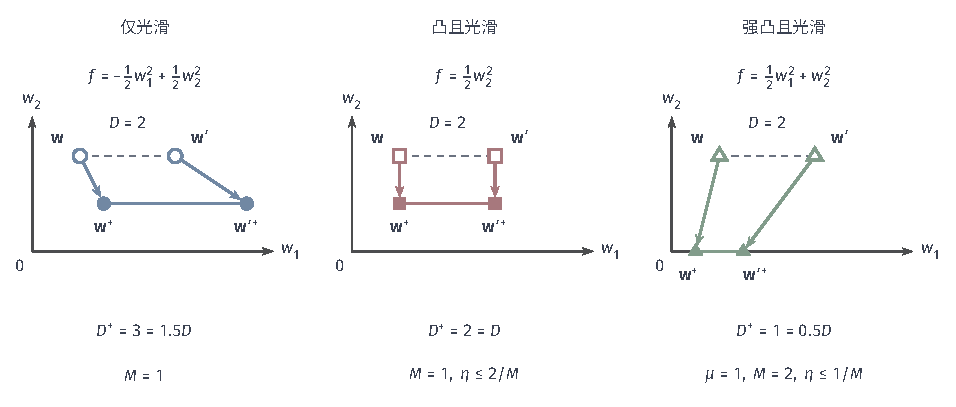
\includegraphics[width=161.957mm]{figures/06-foundations/02-learning-theory/tikz/learning-theory-curvature-stability/figure.pdf}
  \caption{同一梯度更新如何影响参数距离。三个参数平面使用相同尺度，初值均为$\bm w=(1,2)^\top$、$\bm w'=(3,2)^\top$，步长均为$\eta=1/2$。空心标记表示初值，实心标记表示$\bm w^+=\bm w-\eta\nabla f(\bm w)$及$\bm w'^{+}$；箭头表示各自的梯度步，虚线和实线连接更新前后的两点。图中二次函数的梯度步给出精确距离$D^+=3,2,1$，并非一般情形的距离等式。凸且$M$-光滑时，$\eta\leq2/M$保证不扩张；满足强凸光滑条件时，$\eta\leq1/M$保证至多以$1-\mu\eta$收缩。仅有光滑性不能排除扩张。}
  \label{fig:stability-curvature}
\end{figure*}

\paragraph{全梯度下降的距离递推}

全梯度每步都用到被替换的观测，扰动不是随机出现，而是每步都以权重$1/n$出现。把$S'$上的一步写成$\bm w'-\eta\nabla\hat R_S(\bm w')-\eta[\nabla\hat R_{S'}(\bm w')-\nabla\hat R_S(\bm w')]$，后一项只含被替换观测的两个梯度之差，范数至多$2L/n$。若$\hat R_S$凸且$M$-光滑、$\eta_t\leq2/M$，前一部分对两个参数的作用不扩张，于是距离$D_t=\|\bm w^{(t)}-\bm w'^{(t)}\|_2$满足确定性的递推
\[
 D_{t+1}\leq D_t+\frac{2L\eta_t}{n},\qquad D_0=0,
 \qquad D_T\leq\frac{2L}{n}\sum_{t<T}\eta_t.
\]
全梯度只要求整体经验目标满足凸性与光滑性，因为每步作用于两条轨迹的是同一个$\hat R_S$。若$\hat R_S$在整体上还是$\mu$-强凸的，且$\eta_t=\eta\leq1/M$，共同部分以$1-\mu\eta$收缩，递推变为$D_{t+1}\leq(1-\mu\eta)D_t+2L\eta/n$，距离始终不超过$2L/(\mu n)$。SGD不同：每步作用的是单条观测的梯度，下面的强凸结论需要逐观测损失强凸，经验目标强凸不足以保证每个随机更新都收缩。

\paragraph{凸光滑SGD}

\begin{theorem}[凸光滑SGD的稳定性]
\label{thm:convex-sgd-stability}
设$(Z,\mathcal Z)$为可测观测空间，$\ell:\mathbb R^d\times Z\to\mathbb R$可测。对每个$z\in Z$，$\ell(\cdot,z)$可微、凸、$L$-Lipschitz且$M$-光滑，其中$M>0$。固定$n,T\geq1$、确定初值$\bm w^{(0)}\in\mathbb R^d$以及步长$0\leq\eta_t\leq2/M$。任取$Z$上的概率分布$\mathcal P$并令$S\sim\mathcal P^n$。算法内部随机数$U=(i_0,\ldots,i_{T-1})$独立于$S$，由独立且均匀分布于$\{1,\ldots,n\}$的索引组成，并按式~\eqref{eq:sgd-update}更新；令$A_{n,T}(S,U)=\bm w^{(T)}$，比较相邻样本时两次运行共享初值和$U$。则任意只相差一个观测的$S,S'\in Z^n$及任意$z\in Z$都满足
\[
 \left|\mathbb E_U\ell(A_{n,T}(S,U),z)
 -\mathbb E_U\ell(A_{n,T}(S',U),z)\right|\leq\beta_n,
\]
其中
\[
 \beta_n\leq\frac{2L^2}{n}\sum_{t=0}^{T-1}\eta_t.
\]
\end{theorem}
\begin{proof}
令$D_t=\mathbb E_U\|\bm w^{(t)}-\bm w'^{(t)}\|_2$。第$t$步若抽到共同观测，两条轨迹使用同一条损失的梯度步，由前面的余强制性推导，距离不扩张。若以概率$1/n$抽到替换位置，先比较两条轨迹都用$z_i$更新的结果（不扩张），再计入把$z_i$换成$z_i'$产生的额外变化；两个梯度范数都至多为$L$，这部分至多$2\eta_tL$。于是$D_{t+1}\leq D_t+2\eta_tL/n$。从$D_0=0$累加得$D_T\leq(2L/n)\sum_t\eta_t$，再乘以$L$转换为损失差。
\end{proof}

上界取决于步长之和，而不是单独取决于迭代次数。$L=1$、$n=1000$、固定步长$\eta=0.01$时，训练$T=n$步的上界为$2\times0.01\times1000/1000=0.02$，训练$10n$步则为0.2：训练越久，参数能走得越远，泛化差的上界越大。这一结论对每对相邻样本成立，只对共享的索引序列取平均，因此属于第~\ref{sec:algorithmic-stability}节对内部随机性平均后的均匀稳定性。相关分析见Hardt、Recht与Singer\scite{hardt2016sgd}。

\paragraph{逐观测强凸的投影SGD}

若每条观测的损失在可行区域内都强凸，共同观测上的更新还会缩小已有距离。早期替换造成的影响随后续更新衰减，新产生的影响不再简单累加。下面在闭凸集上投影，使参数留在条件成立的区域内；强凸性和梯度有界都只在该区域要求，因为非平凡函数不可能在整个欧氏空间上既全局强凸又梯度有界。

\begin{theorem}[强凸投影SGD的稳定性]
\label{thm:strongly-convex-sgd-stability}
设$(Z,\mathcal Z)$为可测观测空间，$\mathcal W\subseteq\mathbb R^d$是非空闭凸集，$\mathcal O\supseteq\mathcal W$为开集。设$\ell:\mathcal O\times Z\to\mathbb R$可测，每个$\ell(\cdot,z)$在$\mathcal O$上二阶连续可微，且对任意$\bm w\in\mathcal W$、$z\in Z$，
\[
 \mu\bm I\preceq\nabla^2\ell(\bm w,z)\preceq M\bm I,
 \qquad \|\nabla\ell(\bm w,z)\|_2\leq L,
\]
其中$0<\mu\leq M$。固定$n,T\geq1$、初值$\bm w^{(0)}\in\mathcal W$及步长$0<\eta\leq1/M$，内部随机数$U$同定理~\ref{thm:convex-sgd-stability}，并更新$\bm w^{(t+1)}=\Pi_{\mathcal W}(\bm w^{(t)}-\eta\nabla\ell(\bm w^{(t)},z_{i_t}))$。令$A_{n,T}(S,U)=\bm w^{(T)}$，相邻样本上共享初值和$U$。则任意只相差一个观测的$S,S'$及任意$z\in Z$都满足
\[
 \left|\mathbb E_U\ell(A_{n,T}(S,U),z)
 -\mathbb E_U\ell(A_{n,T}(S',U),z)\right|\leq\beta_{n,T},
\]
其中
\[
 \beta_{n,T}\leq\frac{2L^2}{\mu n}\bigl(1-(1-\mu\eta)^T\bigr)\leq\frac{2L^2}{\mu n}.
\]
\end{theorem}
\begin{proof}
共同观测上，梯度步之差为$(\bm I-\eta\bm H)(\bm u-\bm v)$，$\bm I-\eta\bm H$的特征值在$[1-\eta M,1-\eta\mu]\subseteq[0,1-\mu\eta]$内，所以距离至多乘以$1-\mu\eta$；投影不扩大距离。令$D_t=\mathbb E_U\|\bm w^{(t)}-\bm w'^{(t)}\|_2$，抽中替换位置的概率为$1/n$，命中时新增扰动至多$2L\eta$，故$D_{t+1}\leq(1-\mu\eta)D_t+2L\eta/n$，$D_0=0$。求和几何级数得$D_T\leq\frac{2L}{\mu n}(1-(1-\mu\eta)^T)$，再乘以$L$即得结论。
\end{proof}

图~\ref{fig:trajectory-distance}用一维例子模拟三种情形下两条轨迹的平均距离。样本为$[-0.5,0.5]$上等距的20个点，相邻样本把$-0.5$换成$0.5$，步长$\eta=0.1$，对4000条共享索引序列取平均。线性损失$\ell=-zw$凸且光滑（$L=0.5$），梯度与参数无关，每次抽中替换位置都使距离恰好增加$2L\eta=0.1$，平均距离与上界$2L\eta t/n$重合：凸情形的线性增长界在这里取到等号。平方损失在$[-1,1]$上投影（$\mu=M=1$、$L=1.5$），平均距离很快稳定在约0.05，上界稳定在$2L/(\mu n)=0.15$：两者都不随$t$增长。非凸损失$1-\cos(w-z)$从峰顶$w=\pi$出发（$L=M=1$），早期距离按放大因子增长，约28\%的轨迹对最终落入相距约$2\pi$的不同谷，平均距离稳定在约1.8；对应的乘积上界在$t=50$时已达11.6。

\begin{figure*}[htbp]
  \centering
  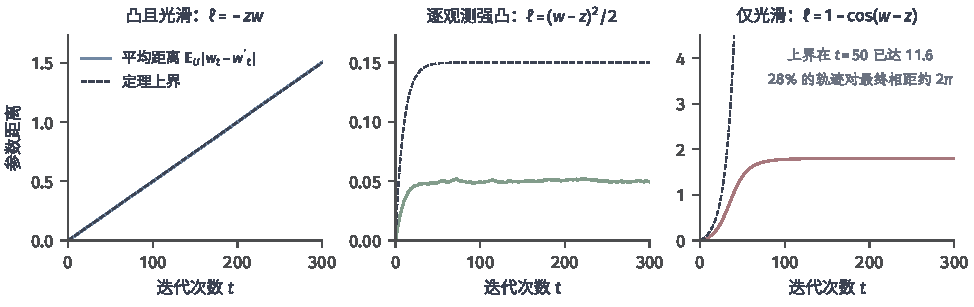
\includegraphics[width=165mm]{figures/06-foundations/02-learning-theory/matplotlib/lt7b-trajectory-distance/figure.pdf}
  \caption{相邻样本上SGD两条轨迹的平均距离。$n=20$，$z_i$为$[-0.5,0.5]$上等距点，相邻样本把$z_1=-0.5$换成$0.5$；$\eta=0.1$，两次运行共享初值与索引序列，对4000条序列取平均（随机种子1）。彩色实线为蒙特卡罗平均距离，黑色虚线为相应定理的上界：左为$2L\eta t/n$，中为$\frac{2L}{\mu n}(1-(1-\mu\eta)^t)$，右为$\frac{2L}{Mn}((1+M\eta)^t-1)$，后者很快超出纵轴范围。}
  \label{fig:trajectory-distance}
\end{figure*}

\paragraph{稳定性与优化误差合并}

强凸投影SGD的结论只改善稳定性，单独得不出学习保证。回到普通凸光滑的条件，把稳定性与式~\eqref{eq:sgd-convex-optimization}的优化误差放进同一个上界。比较决策空间取半径$B$的闭球，每步投影回球内，输出迭代平均。

\begin{theorem}[平均投影SGD的期望风险保证]
\label{thm:averaged-sgd-learning}
设$(Z,\mathcal Z)$为可测观测空间，$\mathcal W=\{\bm w\in\mathbb R^d:\|\bm w\|_2\leq B\}$，其中$B\geq0$，$\mathcal O\supseteq\mathcal W$为开凸集，$\ell:\mathcal O\times Z\to\mathbb R$可测。对每个$z\in Z$，$\ell(\cdot,z)$在$\mathcal O$上可微且凸，在$\mathcal W$上$L$-Lipschitz且$M$-光滑，其中$M>0$。固定$Z$上的概率分布$\mathcal P$，令$S\sim\mathcal P^n$，并假定$\ell(\bm 0,z)\in L^1(\mathcal P)$。令内部随机数$U$同定理~\ref{thm:convex-sgd-stability}，取$n,T\geq1$、初值$\bm w^{(0)}=\bm 0$和固定步长$0<\eta\leq2/M$，更新$\bm w^{(t+1)}=\Pi_{\mathcal W}(\bm w^{(t)}-\eta\nabla\ell(\bm w^{(t)},z_{i_t}))$，输出$\bar{\bm w}=T^{-1}\sum_{t=0}^{T-1}\bm w^{(t)}$。则
\[
 \mathbb E_{S,U}R_{\mathcal P}(\bar{\bm w})-\inf_{\bm w\in\mathcal W}R_{\mathcal P}(\bm w)
 \leq\frac{2L^2\eta T}{n}+\frac{B^2}{2\eta T}+\frac{\eta L^2}{2}.
\]
若$B,L>0$，取$T=n$和$\eta=B/(L\sqrt n)\leq2/M$，右侧不超过$3LB/\sqrt n$。
\end{theorem}
\begin{proof}
若$B=0$，可行集只有$\bm 0$，结论立即成立；以下设$B>0$。投影不扩大距离，因此定理~\ref{thm:convex-sgd-stability}的轨迹比较仍成立：各步距离的期望至多$2L\eta t/n\leq2L\eta T/n$。平均迭代点之间的距离不超过各步距离的平均，再乘以$L$，得到平均输出的稳定性上界$2L^2\eta T/n$，由定理~\ref{thm:stability-expected-generalization}（对内部随机性平均后的版本），它也是期望泛化差的上界。

固定$S$与任意比较参数$\bm w\in\mathcal W$。初值为零，$\|\bm w\|_2\leq B$，式~\eqref{eq:sgd-convex-optimization}给出$\mathbb E_U\hat R_S(\bar{\bm w})-\hat R_S(\bm w)\leq B^2/(2\eta T)+\eta L^2/2$。对训练样本取期望：固定比较参数的经验风险均值等于$R_{\mathcal P}(\bm w)$，输出一侧再加上期望泛化差上界。这正是定理~\ref{thm:expected-risk-comparison}的组合方式。最后对比较参数取下确界，即得结论；代入所给$T,\eta$，三项依次为$2LB/\sqrt n$、$LB/(2\sqrt n)$与$LB/(2\sqrt n)$。
\end{proof}

第一项估计期望泛化差，后两项估计经验优化误差。令$1/\lambda=\eta T$，正则化界$2L^2/(\lambda n)+\lambda B^2/2$的两项恰好变成这里的前两项：总步长$\eta T$扮演了$1/\lambda$的角色。训练越久，参数能走得越远，稳定性越差，离比较决策也越近。这只是两个上界在形式上的对应，并不说明两种算法输出相同的解。

\paragraph{非凸光滑SGD}

不修改非凸目标，直接分析有限步SGD。沿用相邻样本、相同初值和共享索引序列，每一步要计入两件事：抽中被替换观测时新加入的扰动，以及使用共同观测更新时对已有扰动的放大。

\begin{theorem}[非凸SGD的扰动传播]
\label{thm:nonconvex-sgd-product}
设$(Z,\mathcal Z)$为可测观测空间，$\ell:\mathbb R^d\times Z\to\mathbb R$可测。对每个$z\in Z$，$\ell(\cdot,z)$可微、$L$-Lipschitz且$M$-光滑，其中$M>0$。固定$n,T\geq1$、确定初值$\bm w^{(0)}\in\mathbb R^d$及步长$\eta_t\geq0$；内部随机数$U$同定理~\ref{thm:convex-sgd-stability}，按式~\eqref{eq:sgd-update}更新，令$A_{n,T}(S,U)=\bm w^{(T)}$，相邻样本上共享初值和$U$。则任意只相差一个观测的$S,S'$及任意$z\in Z$都满足
\[
 \left|\mathbb E_U\ell(A_{n,T}(S,U),z)
 -\mathbb E_U\ell(A_{n,T}(S',U),z)\right|\leq\beta_{n,T},
\]
其中
\[
 \beta_{n,T}\leq\frac{2L^2}{n}
 \sum_{t=0}^{T-1}\eta_t\prod_{j=t+1}^{T-1}(1+M\eta_j),
\]
其中空乘积取1。若$S\sim\mathcal P^n$、$U$独立于$S$，且独立测试损失与训练损失均可积，则$|\mathbb E_{S,U}[R_{\mathcal P}(A_{n,T})-\hat R_S(A_{n,T})]|$有同样的上界。
\end{theorem}
\begin{proof}
记两次迭代参数的平均距离为$D_t$。未抽中替换位置时，光滑性给出放大因子$1+M\eta_t$。抽中时，在同一观测的更新之外再加入两个观测的梯度差，范数至多$2L\eta_t$。由抽中概率$1/n$，$D_{t+1}\leq(1+M\eta_t)D_t+2L\eta_t/n$，$D_0=0$。逐步展开，第$t$步产生的扰动乘上此后全部的放大因子；最后乘以$L$得到损失差。第二个结论由定理~\ref{thm:stability-expected-generalization}得到。
\end{proof}

步长固定为$\eta>0$时，几何级数求和给出$\beta_{n,T}\leq\frac{2L^2}{Mn}((1+M\eta)^T-1)$。取$L=M=1$、$\eta=0.01$、$T=1000$：凸SGD的上界为$2\eta T/n=20/n$；这里$(1.01)^{1000}\approx2.1\times10^4$，上界约为$4.2\times10^4/n$，大了约两千倍。这个最坏情形上界允许指数放大，并没有断言实际泛化差都指数增长；图~\ref{fig:trajectory-distance}右图中，实际距离在负曲率区过后就停止增长。它说明的是：仅凭光滑性，无法为任意长的训练给出小的稳定性上界。

还可以利用首次访问替换位置的时间。第一次抽中该位置之前两条轨迹完全相同；若那时步长已经减小，后续的放大就比从第一步开始估计时弱。下面是Hardt、Recht与Singer这一思路的一个常数较宽松的版本\scite{hardt2016sgd}。

\begin{theorem}[递减步长的非凸SGD泛化界]
\label{thm:nonconvex-sgd-decay}
设$(Z,\mathcal Z)$为可测观测空间，$\ell:\mathbb R^d\times Z\to[0,1]$可测。对每个$z\in Z$，$\ell(\cdot,z)$可微、$L$-Lipschitz且$M$-光滑，其中$M>0$。固定$n,T\geq1$、确定初值及$c>0$；内部随机数$U$同前，以$0\leq\eta_t\leq c/(t+1)$按式~\eqref{eq:sgd-update}更新，令$A_{n,T}(S,U)=\bm w^{(T)}$，相邻样本上共享初值与$U$。记$\beta_{n,T}$为对任意相邻样本与任意$z$成立的、对$U$平均后的损失差上界，$a=Mc$。则对任意整数$1\leq t_0\leq T$，
\[
 \beta_{n,T}\leq\frac{t_0}{n}
       +\frac{2L^2}{Mn}\left(\frac{T}{t_0}\right)^a.
\]
特别地，取$t_0=\lceil T^{a/(a+1)}\rceil$，可得
\[
 \beta_{n,T}\leq\frac{1+(1+2L^2/M)T^{a/(a+1)}}{n}.
\]
\end{theorem}
\begin{proof}
前$t_0$次抽样中至少一次选中替换位置的概率不超过$t_0/n$；在这一事件上，用损失取值于$[0,1]$得到损失差至多1。在其补事件上，两条轨迹在时刻$t_0$完全相同，后续索引仍独立均匀，可从$D_{t_0}=0$开始使用上一定理的递推。由$1+u\leq e^u$及调和和的积分上界，
\[
 \prod_{j=t+1}^{T-1}\left(1+\frac a{j+1}\right)
 \leq\left(\frac T{t+1}\right)^a,
\]
所以后续的条件期望损失差至多
\[
 \frac{2cL^2T^a}{n}\sum_{t=t_0}^{T-1}(t+1)^{-a-1}
 \leq\frac{2cL^2T^a}{an}\,t_0^{-a},
\]
这里用了$\sum_{t=t_0}^{T-1}(t+1)^{-a-1}\leq\int_{t_0}^{T}x^{-a-1}\,dx\leq t_0^{-a}/a$。合并两种事件，代入$a=Mc$得第一式；再代入所给$t_0$，利用$T^{a/(a+1)}\leq t_0\leq T^{a/(a+1)}+1$得第二式。
\end{proof}

$t_0$是证明中人为选择的观察时刻：$t_0$越大，前$t_0$步碰到替换位置的概率越大；$t_0$越小，之后承受放大的步数越多。所给$t_0$使两项同阶。固定$L,M,c$并令$T=n$，上界为$n^{-1/(a+1)}$量级；$T$按$n^p$增长且$p<(a+1)/a$时，上界仍趋于零。但到这里只知道训练风险与新数据风险在平均意义下相近，算法可能同时把两者维持在较高水平；稳定性界不能说明算法已达到经验全局最优。

\paragraph{PL条件下的学习保证}

要完成学习保证，把非凸稳定性与式~\eqref{eq:pl-sgd-optimization}的PL优化误差合并。为了同时得到两项，这里在一次训练内保持步长$\eta$不变，并使用乘积型稳定性界。

\begin{theorem}[PL条件下非凸SGD的学习保证]
\label{thm:pl-stability-learning}
设$(Z,\mathcal Z)$为可测观测空间，$\mathcal W\subseteq\mathbb R^d$为非空凸Borel区域，$\mathcal O\supseteq\mathcal W$为开集。设$\ell:\mathcal O\times Z\to\mathbb R$可测，各单样本损失在$\mathcal O$上关于参数可微；存在$M>0$和$L\geq0$，使任意$\bm u,\bm v\in\mathcal W$、$z\in Z$都满足
\[
 \|\nabla\ell(\bm u,z)-\nabla\ell(\bm v,z)\|_2\leq M\|\bm u-\bm v\|_2,
 \qquad
 \|\nabla\ell(\bm u,z)\|_2\leq L.
\]
对每个允许分布$\mathcal P$，令$S\sim\mathcal P^n$。固定初值$\bm w^{(0)}\in\mathcal W$、步长$0<\eta\leq1/M$及$T\geq1$；内部随机数$U$同前，按式~\eqref{eq:sgd-update}以固定步长更新，并假定对所有样本和索引序列，全部迭代点均留在$\mathcal W$内。存在$0<\mu\leq M$及$D\geq0$，使每个样本及其每个迭代点都满足
\[
\begin{aligned}
 \frac12\|\nabla\hat R_S(\bm w^{(t)})\|_2^2
 &\geq\mu\Bigl(\hat R_S(\bm w^{(t)})-\inf_{\bm w\in\mathcal W}\hat R_S(\bm w)\Bigr),\\
 \hat R_S(\bm w^{(0)})-\inf_{\bm w\in\mathcal W}\hat R_S(\bm w)&\leq D.
\end{aligned}
\]
进一步设存在$\nu\geq0$，使对所有$S\in Z^n$和$\bm w\in\mathcal W$都有
\[
 \frac1n\sum_{i=1}^n\|\nabla\ell(\bm w,z_i)-\nabla\hat R_S(\bm w)\|_2^2\leq\nu^2.
\]
假定独立测试损失$\ell(\bm w^{(T)},z)$、训练损失$\ell(\bm w^{(T)},z_i)$及每个固定$\bm w\in\mathcal W$的$\ell(\bm w,z)$均可积，经验风险与期望风险的下确界为有限实数且可测。则
\[
 \mathbb E_{S,U}R_{\mathcal P}(\bm w^{(T)})-\inf_{\bm w\in\mathcal W}R_{\mathcal P}(\bm w)
 \leq\frac{2L^2}{Mn}\bigl((1+M\eta)^T-1\bigr)+D(1-\mu\eta)^T+\frac{M\eta\nu^2}{2\mu}.
\]
\end{theorem}
\begin{proof}
定理~\ref{thm:nonconvex-sgd-product}的轨迹比较给出第一项，它上界期望泛化差。为分析经验优化误差，固定样本及此前的迭代，记$\bm g_t=\nabla\ell(\bm w^{(t)},z_{i_t})$。条件均值为$\nabla\hat R_S(\bm w^{(t)})$，条件二阶矩不超过$\|\nabla\hat R_S(\bm w^{(t)})\|_2^2+\nu^2$。把更新代入光滑性不等式并对当前索引取期望，
\[
 \mathbb E\hat R_S(\bm w^{(t+1)})
 \leq\hat R_S(\bm w^{(t)})-\frac\eta2\|\nabla\hat R_S(\bm w^{(t)})\|_2^2+\frac{M\eta^2\nu^2}{2},
\]
这里用$\eta\leq1/M$把梯度范数平方的系数控制为$-\eta/2$。再用PL条件把这一负项换成当前经验目标差的$-\mu\eta$倍，减去最低经验风险并对此前索引平均，即得式~\eqref{eq:pl-sgd-optimization}，从而$e_T\leq D(1-\mu\eta)^T+M\eta\nu^2/(2\mu)$。这个上界对每份样本都成立。期望超额风险不超过期望泛化差加上平均经验优化误差（定理~\ref{thm:expected-risk-comparison}），两部分相加即得结论。
\end{proof}

增加$T$使第二项下降，却可能增大第一项；固定非零步长且$\nu>0$时，第三项不随$T$下降。全梯度时$\nu=0$，但仍要为全梯度更新建立相应的稳定性界，不能只从公式中删去方差项。要使三项同时趋于零，可随样本量调整整次训练的步长和时长：要求$L,M,D,\nu$有不依赖分布和样本量的上界，PL常数$\mu$有统一的正下界；取$\eta_n=n^{-r}$（$r>0$），在一次训练内保持不变，并令$T_n=\lfloor c_0\log n/\eta_n\rfloor$，其中$0<c_0<1/M$。总步长约为$c_0\log n$，由$(1+M\eta)^T\leq e^{M\eta T}$，三项分别为$O(n^{Mc_0-1})$、$O(n^{-\mu c_0})$与$O(n^{-r})$，都趋于零，在这些统一条件下得到PAC学习保证。非凸性并不自动排除学习，但只证明算法稳定或梯度变小都不够。

\paragraph{提前停止}

式中的折中在凸情形最清楚。定理~\ref{thm:averaged-sgd-learning}的上界$2L^2\eta T/n+B^2/(2\eta T)+\eta L^2/2$中，前一项随训练时长增长，后一项随之下降；在固定$\eta$下对$T$最小化，得到$\eta T=B\sqrt n/(2L)$。按上界选择停止时刻，就是一种\term{提前终止}（early stopping）。但这个时刻只使上界最小，不保证实际测试风险在此最小：上界中的常数是最坏情形的估计，实际泛化差可能远小于$2L^2\eta T/n$（例如图~\ref{fig:trajectory-distance}中强凸情形的距离只有上界的三分之一）。实践中的停止时刻通常由验证样本决定，这又回到模型选择，需要按第~\ref{sec:srm}节或第~\ref{sec:model-selection}节的方式计入选择代价。提前停止与正则化的上界形式相似，也不能推出两种方法得到同一个解。

\subsubsection{隐式偏置}
\label{sec:linear-implicit-bias}
\label{sec:implicit-bias-linear}

前两项回答了“经验目标求解得多好”和“输出对样本有多敏感”。还有一个问题它们没有回答：经验目标有许多个最优解时，算法到底选哪一个？

\paragraph{多个插值解与选解偏好}

取一个训练样本$\bm x=(1,1)^\top$、$y=1$，线性预测$\bm w^\top\bm x$。插值要求$w_1+w_2=1$，直线上的$(1,0)^\top$、$(0,1)^\top$和$(1/2,1/2)^\top$都能完美拟合，却在新输入$(1,0)^\top$上分别预测1、0与$1/2$。经验目标为零不能确定预测函数。从零初始化做梯度下降，梯度$(w_1+w_2-1)(1,1)^\top$的两个分量始终相同，轨迹保持$w_1=w_2$，只能趋于中点。直线上其他点写成$(1/2+a,1/2-a)^\top$，范数平方为$1/2+2a^2$，所以中点正是范数最小者。

这种由初始化、损失、参数化和更新规则共同产生、却没有显式写进目标函数的选解倾向，称为\term{隐式偏置}（implicit bias）。“偏置”指算法偏好某一类解，不是风险分解中的近似误差；“隐式”指这种偏好没有通过正则项等方式声明。参数化的影响可以用标量模型$wx$看清：直接训练$w$时，若损失对$w$的梯度为$g$，每步更新量都是$-\eta g$，与$w$的大小无关；改写成$w=uv$后，$u$与$v$的更新量分别是$-\eta gv$与$-\eta gu$，$w$本身的变化约为$-\eta g(u^2+v^2)$，系数已经较大时变化更快，接近零时几乎不动。两种写法表示同一族函数，训练却走出不同的路线。深层参数化的具体动力学留到第~\ref{sec:deep-implicit-bias}节；这里在两个能算清楚的线性模型中证明选解机制，再说明它们怎样进入风险分析。

\paragraph{欠定线性回归的最小范数解}

\begin{theorem}[梯度下降的最小范数选择]
\label{thm:min-norm-interpolation}
\label{thm:learning-gradient-descent-minimum-norm}
设$n,d\geq1$且$d>n$，$\bm X\in\mathbb R^{n\times d}$满行秩，$\bm y\in\mathbb R^n$。对$\hat R_S(\bm w)=\|\bm X\bm w-\bm y\|_2^2/(2n)$，以步长$0<\eta<2n/\|\bm X\|_2^2$运行全梯度下降$\bm w^{(t+1)}=\bm w^{(t)}-\eta\nabla\hat R_S(\bm w^{(t)})$。从$\bm w^{(0)}=\bm 0$出发，
\begin{equation}
 \bm w^{(t)}\longrightarrow\widehat{\bm w}
 =\bm X^\top(\bm X\bm X^\top)^{-1}\bm y
 =\argmin_{\bm X\bm w=\bm y}\|\bm w\|_2.
 \label{eq:learning-minimum-norm-interpolator}
\end{equation}
从一般初值$\bm w^{(0)}$出发，$\bm w^{(t)}\to\widehat{\bm w}+(\bm I-\bm P_X)\bm w^{(0)}$，其中$\bm P_X=\bm X^\top(\bm X\bm X^\top)^{-1}\bm X$是向行空间$\operatorname{range}(\bm X^\top)$的正交投影。
\end{theorem}
\begin{proof}
每次更新的增量为$-\eta\bm X^\top(\bm X\bm w^{(t)}-\bm y)/n$，是$\bm X$各行的线性组合，落在行空间中。所以零空间分量$(\bm I-\bm P_X)\bm w^{(t)}$在整个训练中保持为$(\bm I-\bm P_X)\bm w^{(0)}$。再看残差$\bm e^{(t)}=\bm X\bm w^{(t)}-\bm y$：
\[
 \bm e^{(t+1)}=\left(\bm I-\frac\eta n\bm X\bm X^\top\right)\bm e^{(t)}.
\]
满行秩使$\bm X\bm X^\top$正定，步长条件使括号内全部特征值的绝对值小于1，所以$\bm e^{(t)}\to\bm 0$，行空间分量收敛到唯一满足$\bm X\bm w=\bm y$的行空间向量，即$\widehat{\bm w}$。两部分相加得到一般初值的极限，零初始化时零空间分量为零。任意插值解可写成
\begin{equation}
 \bm w=\widehat{\bm w}+\bm v,\qquad\bm v\in\operatorname{null}(\bm X);
 \label{eq:learning-interpolator-decomposition}
\end{equation}
行空间与零空间正交，$\|\bm w\|_2^2=\|\widehat{\bm w}\|_2^2+\|\bm v\|_2^2$，当且仅当$\bm v=\bm 0$时范数最小。
\end{proof}

证明的核心是一个几何事实：梯度$\bm X^\top(\cdot)$总落在训练输入张成的行空间里，从零出发的迭代永远得不到零空间方向的分量。图~\ref{fig:learning-minimum-norm}画出零初始化的情形。图~\ref{fig:min-norm-initialization}再从$\bm w^{(0)}=(-0.6,0)^\top$出发：它的行空间分量为$(-0.3,-0.3)^\top$，零空间分量为$\bm v=(-0.3,0.3)^\top$。以步长$1/4$更新，残差每步减半，迭代依次为$(-0.2,0.4)^\top$、$(0,0.6)^\top$、$(0.1,0.7)^\top$，极限为$(0.2,0.8)^\top=\widehat{\bm w}+\bm v$：轨迹与零初始化的轨迹平行，只是整体平移了$\bm v$。它的范数平方为0.68，大于最小值0.5，在新输入$(1,0)^\top$上预测0.2而不是0.5。初值是选解规则的一部分。

\begin{figure}[htbp]
  \centering
  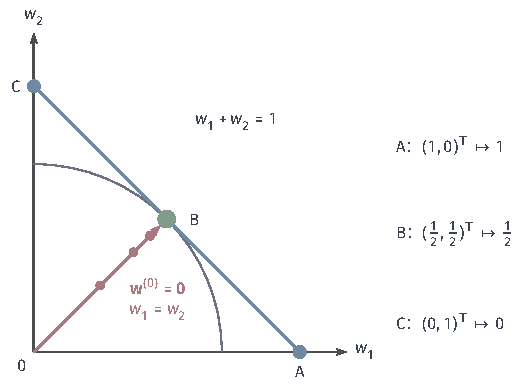
\includegraphics[width=88.805mm]{figures/06-foundations/02-learning-theory/tikz/learning-theory-minimum-norm/figure.pdf}
  \caption{一个训练观测对应多个插值参数。直线上的A、B、C都使输入$(1,1)^\top$的预测为1，右侧列出它们对同一个新输入$\bm x_{\mathrm{new}}=(1,0)^\top$的预测。对半平方损失从零初始化，图中以步长$1/4$画出前三次更新，轨迹趋向B；细弧表示经过B的欧氏范数等值线，说明B是插值直线上距离原点最近的点。这个教学例子解释选解规则，不给出新输入的真实标签或泛化保证。}
  \label{fig:learning-minimum-norm}
\end{figure}

\begin{figure}[htbp]
  \centering
  % 欠定线性回归中初始化的零空间分量被梯度下降原样保留。
% 一个训练观测 x=(1,1)^T、y=1，半平方损失 (w1+w2-1)^2/2，步长 eta=1/4。
% 残差 r=w1+w2-1 每步乘 1-2eta=1/2；更新 w <- w - eta r (1,1)^T。
% 零初始化：0 -> (.25,.25) -> (.375,.375) -> (.4375,.4375) -> B=(.5,.5)。
% 初值 w0=(-0.6,0)：行空间分量 (-0.3,-0.3)，零空间分量 v=(-0.3,0.3)；
%   迭代 (-0.2,0.4) -> (0,0.6) -> (0.1,0.7) -> 极限 B+v=(0.2,0.8)。
% 坐标：x=1mm,y=1mm，参数每单位 40 mm。
\begingroup
\begin{tikzpicture}[figure picture,x=1mm,y=1mm]
  \def\s{40}
  % 坐标轴
  \draw[-{Stealth[length=1.6mm]},FigureStroke,line width=.6pt] (-0.85*\s,0)--(1.3*\s,0) node[right]{$w_1$};
  \draw[-{Stealth[length=1.6mm]},FigureStroke,line width=.6pt] (0,-0.25*\s)--(0,1.3*\s) node[above]{$w_2$};
  \node[figure note,anchor=north east] at (0,0) {$0$};
  % 行空间方向 w1=w2 与零空间方向 w1=-w2
  \draw[FigureMuted,line width=.4pt,dash pattern=on 1.5pt off 1.5pt] (-0.2*\s,-0.2*\s)--(1.15*\s,1.15*\s);
  \node[figure note,anchor=west] at (1.0*\s,1.12*\s) {行空间 $w_1=w_2$};
  \draw[FigureMuted,line width=.4pt,dash pattern=on 1.5pt off 1.5pt] (0.2*\s,-0.2*\s)--(-0.62*\s,0.62*\s);
  \node[figure note,anchor=east] at (-0.62*\s,0.66*\s) {零空间 $w_1=-w_2$};
  % 插值直线
  \draw[FigureBlue,line width=1.1pt] (-0.25*\s,1.25*\s)--(1.25*\s,-0.25*\s);
  \node[font=\figurefont\footnotesize,text=FigureBlue,anchor=west] at (1.04*\s,-0.06*\s) {插值解 $w_1+w_2=1$};
  % 零初始化轨迹
  \draw[FigureRed,line width=.9pt,-{Stealth[length=1.5mm]}] (0,0)--(0.25*\s,0.25*\s);
  \draw[FigureRed,line width=.9pt,-{Stealth[length=1.5mm]}] (0.25*\s,0.25*\s)--(0.375*\s,0.375*\s);
  \draw[FigureRed,line width=.9pt] (0.375*\s,0.375*\s)--(0.5*\s,0.5*\s);
  \foreach \p in {0.25,0.375,0.4375}{\fill[FigureRed] (\p*\s,\p*\s) circle (0.7);}
  \fill[FigureRed] (0.5*\s,0.5*\s) circle (1.3);
  \node[font=\figurefont\footnotesize,text=FigureRed,anchor=north west] at (0.56*\s,0.40*\s) {$\widehat{\bm w}=(0.5,0.5)$};
  % 非零初值轨迹
  \fill[FigureYellow] (-0.6*\s,0) circle (1.1);
  \node[font=\figurefont\footnotesize,anchor=north] at (-0.6*\s,-1.5) {$\bm w^{(0)}=(-0.6,0)$};
  \draw[FigureYellow!80!black,line width=.9pt,-{Stealth[length=1.5mm]}] (-0.6*\s,0)--(-0.2*\s,0.4*\s);
  \draw[FigureYellow!80!black,line width=.9pt,-{Stealth[length=1.5mm]}] (-0.2*\s,0.4*\s)--(0,0.6*\s);
  \draw[FigureYellow!80!black,line width=.9pt] (0,0.6*\s)--(0.2*\s,0.8*\s);
  \foreach \a/\b in {-0.2/0.4,0/0.6,0.1/0.7}{\fill[FigureYellow!80!black] (\a*\s,\b*\s) circle (0.7);}
  \fill[FigureYellow!80!black] (0.2*\s,0.8*\s) circle (1.3);
  \node[font=\figurefont\footnotesize,anchor=south west] at (0.22*\s,0.82*\s) {$\widehat{\bm w}+\bm v=(0.2,0.8)$};
  % 零空间分量 v
  \draw[FigureInk,line width=.6pt,-{Stealth[length=1.5mm]}] (0.5*\s,0.5*\s)--(0.2*\s,0.8*\s);
  \node[figure edge label] at (0.38*\s,0.62*\s) {$\bm v$};
  \draw[FigureInk,line width=.6pt,-{Stealth[length=1.5mm]}] (0,0)--(-0.3*\s,0.3*\s);
  \node[figure edge label,anchor=north east] at (-0.15*\s,0.13*\s) {$\bm v$};
\end{tikzpicture}
\endgroup

  \caption{初始化的零空间分量被梯度下降原样保留。训练观测与步长同图~\ref{fig:learning-minimum-norm}。红色轨迹从原点出发，沿行空间方向$w_1=w_2$趋于最小范数解$\widehat{\bm w}$；黄色轨迹从$\bm w^{(0)}=(-0.6,0)^\top$出发，各步与红色轨迹平行，趋于$\widehat{\bm w}+\bm v$。两段黑色箭头都是零空间分量$\bm v=(-0.3,0.3)^\top$：它在初值中存在，在极限中原样保留。}
  \label{fig:min-norm-initialization}
\end{figure}

选解规则确定以后，还要回答它在新输入上误差有多大。同一个最小范数解在不同数据分布下的表现可以很不相同：真实关系落在训练样本张成的方向上时误差小，主要落在训练样本看不到的方向上时误差大。因此要在明确的数据生成模型下逐项计算误差。设存在真实参数$\bm w_\star$，测试标签$y=\bm x^\top\bm w_\star+\xi$，$\mathbb E[\xi\mid\bm x]=0$且$\mathbb E\xi^2<\infty$；记输入的未中心化二阶矩矩阵$\bm\Sigma=\mathbb E[\bm x\bm x^\top]$，它记录输入在各方向上的平方规模。风险用完整平方损失$R(\bm w)=\mathbb E[(\bm x^\top\bm w-y)^2]$；它与优化用的半平方损失只差常数因子，不改变极限。由$\bm x^\top\bm w-y=\bm x^\top(\bm w-\bm w_\star)-\xi$，平方后交叉项因条件零均值而消失，得到
\[
 R(\bm w)-R(\bm w_\star)=\|\bm w-\bm w_\star\|_{\bm\Sigma}^2,
 \qquad\|\bm v\|_{\bm\Sigma}^2=\bm v^\top\bm\Sigma\bm v.
\]
回归超额风险等于参数误差按输入二阶矩加权的长度：参数在输入很少出现的方向上偏差再大，对预测的影响也很小。

\begin{theorem}[基于最小范数的回归期望风险]
\label{thm:minimum-norm-risk-decomposition}
设测试输入$\bm x\in\mathbb R^d$满足$\mathbb E\|\bm x\|_2^2<\infty$，$\bm\Sigma=\mathbb E[\bm x\bm x^\top]$，测试标签$y=\bm x^\top\bm w_\star+\xi$，$\mathbb E[\xi\mid\bm x]=0$，$\mathbb E\xi^2<\infty$。固定满行秩设计矩阵$\bm X\in\mathbb R^{n\times d}$，$n<d$，训练标签$\bm y=\bm X\bm w_\star+\bm\xi$，其中$\mathbb E[\bm\xi\mid\bm X]=\bm 0$、$\mathbb E[\bm\xi\bm\xi^\top\mid\bm X]=\sigma^2\bm I_n$，$\sigma^2\geq0$。令$\widehat{\bm w}=\bm X^\top(\bm X\bm X^\top)^{-1}\bm y$。则
\begin{equation}
 \mathbb E_{\bm\xi\mid\bm X}[R(\widehat{\bm w})-R(\bm w_\star)]
 =\|(\bm I-\bm P_X)\bm w_\star\|_{\bm\Sigma}^2
 +\sigma^2\operatorname{tr}\left[\bm\Sigma\bm X^\top(\bm X\bm X^\top)^{-2}\bm X\right].
 \label{eq:minimum-norm-prediction-risk}
\end{equation}
\end{theorem}
\begin{proof}
把$\bm y=\bm X\bm w_\star+\bm\xi$代入$\widehat{\bm w}$，记$\bm M=\bm X^\top(\bm X\bm X^\top)^{-1}$，得$\widehat{\bm w}=\bm P_X\bm w_\star+\bm M\bm\xi$，于是
\[
 \widehat{\bm w}-\bm w_\star=-(\bm I-\bm P_X)\bm w_\star+\bm M\bm\xi.
\]
第一项与噪声无关，只由真实参数和训练样本覆盖的方向决定；第二项是训练标签中的噪声被写进参数的部分。在$\bm\Sigma$半范数下展开平方，交叉项因$\mathbb E[\bm\xi\mid\bm X]=\bm 0$而期望为零。噪声项$\mathbb E\|\bm M\bm\xi\|_{\bm\Sigma}^2=\mathbb E\operatorname{tr}(\bm\Sigma\bm M\bm\xi\bm\xi^\top\bm M^\top)=\sigma^2\operatorname{tr}(\bm\Sigma\bm M\bm M^\top)$，而$\bm M\bm M^\top=\bm X^\top(\bm X\bm X^\top)^{-2}\bm X$，即得迹表达式。
\end{proof}

两项误差各有直观含义。第一项来自训练样本没有覆盖的方向：$(\bm I-\bm P_X)\bm w_\star$是真实参数在训练样本完全看不到的那部分，零初始化不会凭空补出它，最小范数解在这些方向上取零。二维例子中若$\bm w_\star=(1,0)^\top$，训练样本只看到它在$(1,1)$方向的投影，学到$(1/2,1/2)^\top$，在$(1,-1)$方向丢失了$(1/2,-1/2)^\top$。第二项来自拟合训练噪声：训练输入接近线性相关时，$(\bm X\bm X^\top)^{-1}$在相应方向上很大，会把噪声放大后写进参数。若设计矩阵也随机且右侧可积，再对$\bm X$平均即得随机设计下的平均风险。

一个精确算例取无噪声、各向同性输入：$\bm x_i\sim\mathcal N(\bm 0,\bm I_d)$，$\sigma=0$，$\bm\Sigma=\bm I_d$。随机$n$维行空间具有旋转对称性，期望投影只能是单位矩阵的倍数；由$\operatorname{tr}(\bm P_X)=n$知$\mathbb E\bm P_X=(n/d)\bm I_d$，于是
\begin{equation}
 \mathbb E_S[R(\widehat{\bm w})-R(\bm w_\star)]
 =\left(1-\frac nd\right)\|\bm w_\star\|_2^2,
 \qquad n<d.
 \label{eq:isotropic-minimum-norm-risk}
\end{equation}
$\|\bm w_\star\|_2=1$、$d=100$、$n=10$时，经验风险为零，平均超额风险却为0.9；要使它不超过$\varepsilon<1$，需要$n\geq d(1-\varepsilon)$。最小范数本身不保证低风险。

\paragraph{良性过拟合}
\phantomsection\label{sec:benign-overfitting}

上面的各向同性算例中，插值失败的原因是偏差项：样本只覆盖了$d$个方向中的$n$个。若训练标签含噪声，完全插值又要把噪声写进参数。按经典的直觉，含噪样本被完全拟合时，测试风险不会好。Bartlett、Long、Lugosi与Tsigler研究了一个问题：线性回归中的最小范数插值能否一边完全拟合含噪样本，一边保持很小的超额风险\scite{bartlett2020benign}？若能，就称为\term{良性过拟合}（benign overfitting）。

他们的设定是：输入$\bm x=\bm\Sigma^{1/2}\bm u$，$\bm u$的分量独立且次高斯；标签$y=\bm x^\top\bm w_\star+\xi$，噪声条件均值为零、方差为$\sigma^2$；估计量是式~\eqref{eq:learning-minimum-norm-interpolator}的最小范数插值，风险是对新观测的超额平方风险。把$\bm\Sigma$的特征值从大到小记为$\lambda_1\geq\lambda_2\geq\cdots$，定义两种有效秩
\[
 r_k(\bm\Sigma)=\frac{\sum_{i>k}\lambda_i}{\lambda_{k+1}},
 \qquad
 R_k(\bm\Sigma)=\frac{(\sum_{i>k}\lambda_i)^2}{\sum_{i>k}\lambda_i^2}.
\]
它们都衡量第$k$个之后的“尾部”方向有多少个分量规模相当：尾部特征值全相等时，二者都等于尾部的维数。记$k^*$为使$r_k(\bm\Sigma)$不小于某个常数倍$n$的最小$k$。他们证明，以高概率（对训练输入），超额风险的上界由三部分组成：与$\|\bm w_\star\|_2^2\|\bm\Sigma\|$及$\sqrt{r_0(\bm\Sigma)/n}$相关的偏差项，以及与$\sigma^2(k^*/n+n/R_{k^*}(\bm\Sigma))$相关的噪声项；噪声项还有同阶的下界。由此得到的刻画是：插值是良性的，大致需要$r_0(\bm\Sigma)/n$、$k^*/n$与$n/R_{k^*}(\bm\Sigma)$都趋于零。准确的常数与概率条件以原文为准。

这一刻画的读法是把谱分成两部分。前$k^*$个大方向像普通的低维回归，噪声代价约为$k^*/n$，需要$k^*$远小于$n$；其余的尾部方向数量很多、各自很小，噪声被分散到这些方向上，每个方向只吸收一点，代价约为$n/R_{k^*}$，需要尾部的有效维数远大于$n$。用前面的各向同性例子对照：$\bm\Sigma=\bm I_d$时$r_0=d$，$d\gg n$使$r_0/n$很大，偏差项不小，正与式~\eqref{eq:isotropic-minimum-norm-risk}的0.9一致。若改为前10个方向特征值为1、其余$10^6$个方向特征值为$10^{-5}$、$n=1000$，则尾部特征值之和为10，$r_0\approx20$，$r_0/n\approx0.02$；尾部有效秩约$10^6$，$n/R\approx10^{-3}$；大方向的代价$k/n\approx0.01$。三个比值都小，属于良性的范围，前提是真实参数主要落在前10个方向上。

结论有几处要说准确。第一，良性过拟合依赖协方差谱，不由“参数量超过样本量”单独决定：各向同性的$d\gg n$恰好不是良性的。第二，原文的上界针对随机训练输入，以高概率成立；式~\eqref{eq:minimum-norm-prediction-risk}则是固定设计下对噪声的条件期望，二者对象不同，前者还需要对设计矩阵的集中性论证。第三，这是线性模型、平方损失和最小范数插值的结论，换成别的插值解、别的损失或非线性模型，要重新检查。

\paragraph{可分逻辑回归的最大间隔方向}

逻辑分类与平方回归的参数极限不同。对线性可分数据，把参数沿正确分类的方向不断放大，每个样本的$y\bm w^\top\bm x$都变大，$\log(1+e^{-y\bm w^\top\bm x})$持续下降。经验风险的下确界为零，却没有有限参数能达到它，梯度下降会让参数范数一直增长。参数本身不收敛，有意义的问题是归一化方向$\bm w/\|\bm w\|_2$趋于哪里；分类结果只取决于方向，这也正是“最终得到哪条判定边界”。

取$y_i\in\{-1,1\}$，单位方向$\bm u$的最小经验间隔为$\min_iy_i\bm u^\top\bm x_i$，即离判定边界最近的训练样本到边界的距离。把未归一化间隔固定为至少1再最小化范数，等价于最大化单位方向的这个最小距离，得到硬间隔支持向量机的几何目标：在所有能分开训练样本的边界中，选离两类最近样本都最远的那一条。

\begin{theorem}[逻辑回归梯度下降的最大间隔方向]
\label{thm:max-margin-direction}
\label{thm:logistic-max-margin-direction}
设$n,d\geq1$，$\bm x_i\in\mathbb R^d$、$y_i\in\{-1,+1\}$，且存在$\bm w$使$y_i\bm w^\top\bm x_i>0$对所有$i$成立。令$\bm X\in\mathbb R^{n\times d}$以$\bm x_i^\top$为第$i$行，定义
\[
 \hat R_S(\bm w)=\frac1n\sum_{i=1}^{n}\log(1+e^{-y_i\bm w^\top\bm x_i}),
 \qquad
 \bm w^{(t+1)}=\bm w^{(t)}-\eta\nabla\hat R_S(\bm w^{(t)}).
\]
从任意$\bm w^{(0)}$出发，取$0<\eta<n/\|\bm X\|_2^2$。则$\|\bm w^{(t)}\|_2\to\infty$，且
\[
 \frac{\bm w^{(t)}}{\|\bm w^{(t)}\|_2}
 \longrightarrow\frac{\widehat{\bm w}_{\mathrm{svm}}}{\|\widehat{\bm w}_{\mathrm{svm}}\|_2},
\]
其中
\[
 \widehat{\bm w}_{\mathrm{svm}}
 =\argmin_{\bm w}\tfrac12\|\bm w\|_2^2
 \quad\text{满足}\quad y_i\bm w^\top\bm x_i\geq1\ (1\leq i\leq n).
\]
\end{theorem}
以下证明使用Soudry等对可分逻辑回归的渐近展开\scite{soudry2018implicit}。
\begin{proof}[证明（使用外部渐近结果）]
在上述步长条件下，所引结果给出
\[
 \bm w^{(t)}=\widehat{\bm w}_{\mathrm{svm}}\log t+\bm\rho^{(t)},
\]
其中$\|\bm\rho^{(t)}\|_2=O(\log\log t)$。由于$\log\log t/\log t\to0$，除以$\log t$后取极限得到$\widehat{\bm w}_{\mathrm{svm}}$。该向量非零，故参数范数发散，归一化方向收敛到所述方向。渐近展开本身是外部结果，这里只证明由它到方向收敛的推论。
\end{proof}

从每个样本对梯度的贡献可以理解这一选择：
\[
 -\nabla\hat R_S(\bm w)
 =\frac1n\sum_{i=1}^{n}\frac{y_i\bm x_i}{1+e^{y_i\bm w^\top\bm x_i}}.
\]
样本$i$的系数$1/(1+e^{y_i\bm w^\top\bm x_i})$随间隔快速衰减：间隔为0时为0.5，为1时约0.27，为5时只剩约0.0067。参数范数增长后，离边界远的样本间隔越来越大，对更新方向的影响迅速消失；离边界最近的样本衰减最慢，最终主导更新方向，梯度下降于是不断把方向调向使这些样本离边界更远的位置。这与支持向量机只由支持向量决定的性质相对应。即使全部训练样本都已分对，逻辑损失仍在推动方向变化。这段机制解释不能代替方向极限的证明。

图~\ref{fig:logistic-max-margin}在一个二维可分样本上运行这一过程。正类为$(1,0.25)$、$(2.5,2)$、$(0.4,1.6)$、$(3,0.6)$、$(1.8,1.1)$，负类为它们的相反数，从零初始化，步长$\eta=0.9n/\|\bm X\|_2^2\approx0.179$。最大间隔方向与$x_1$轴夹约$24.0^\circ$，最小归一化间隔$\gamma_{\mathrm{svm}}\approx1.015$，支持向量为$(1,0.25)$、$(0.4,1.6)$及其相反数。参数范数在$t=10^2,10^4,10^6$时约为2.24、6.30、10.79，大致随$\log t$线性增长；方向与最大间隔方向的夹角先从$t=1$时的$8.6^\circ$升到$t=100$时的$13.6^\circ$，再缓慢下降到$t=10^6$时的$6.7^\circ$；最小归一化间隔相应地先从0.978降到0.945，再升到0.988，仍低于$\gamma_{\mathrm{svm}}$。方向收敛是渐近结论，速率只有$1/\log t$量级，也不保证每一步间隔都改善。

\begin{figure*}[htbp]
  \centering
  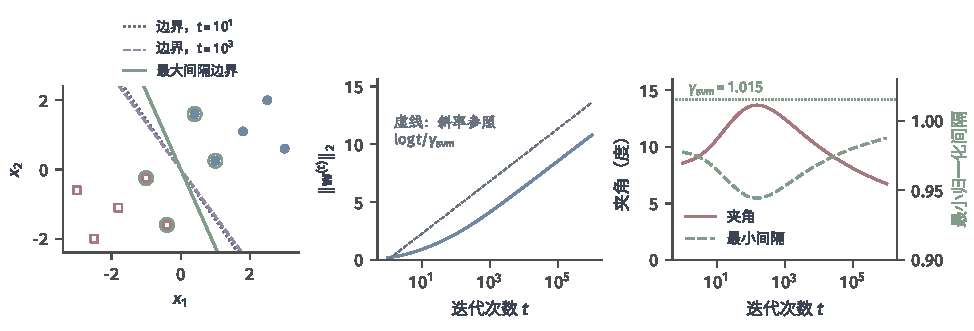
\includegraphics[width=165mm]{figures/06-foundations/02-learning-theory/matplotlib/lt7b-logistic-max-margin/figure.pdf}
  \caption{可分逻辑回归上的梯度下降。左：十个训练点（实心为正类，空心为负类），绿线为最大间隔边界，圆圈为支持向量，灰点线与紫虚线为$t=10$与$t=10^3$时由$\bm w^{(t)}$确定的边界。中：参数范数随迭代次数（对数横轴）增长，虚线是斜率参照$\log t/\gamma_{\mathrm{svm}}$。右：方向与最大间隔方向的夹角（实线，左纵轴）和最小归一化间隔（虚线，右纵轴）；点线为$\gamma_{\mathrm{svm}}$。全梯度下降，零初始化，$\eta\approx0.179$，记录到$t=10^6$。}
  \label{fig:logistic-max-margin}
\end{figure*}

方向的选择可以接到第~\ref{sec:rademacher-complexity}节的线性间隔风险界（定理~\ref{thm:linear-margin-risk}）：对事先固定的阈值$\gamma>0$，单位范数线性分类器的零一风险不超过训练集上归一化间隔不大于$\gamma$的比例，加上与$r/(\gamma\sqrt n)$同阶的复杂度项及置信项，其中$r$为输入范数的上界。若训练数据的最大归一化间隔严格大于预定的$\gamma$，定理~\ref{thm:max-margin-direction}保证充分训练后的方向也超过这一阈值，经验项为零。以复杂度项$2r/(\gamma\sqrt n)$计，输入归一化为$r=1$、$\gamma=0.1$时，要把它降到0.05需要$n\geq1.6\times10^5$，与输入维数无关。

这一推论有三处边界。第一，进入风险的是归一化间隔：统一放大参数会同时放大原始间隔和范数，比值不变，只有方向变化才可能改善它。第二，方向收敛不给出有限步的保证：像图~\ref{fig:logistic-max-margin}那样，有限步时的最小间隔可能低于最大间隔，经验项需要按实际达到的间隔计算。第三，样本可分不保证随$n$增长仍有固定的正间隔；若有标签噪声，靠记住噪声样本得到的可分边界间隔可能很小，界也随之失效。

\paragraph{三项结论的关系}

选到结构简单的解，不等于替换一个样本后仍选到相近的解。取两个几乎平行的训练输入$\bm x_1=(1,0,0)^\top$、$\bm x_2=(1,\epsilon,0)^\top$，$\epsilon=10^{-3}$。标签为$(0,0)$时最小范数解为$\bm 0$；只把第二个标签改为0.01，插值要求$w_1=0$、$w_1+\epsilon w_2=0.01$，最小范数解变为$(0,10,0)^\top$。标签改变0.01，参数移动了10；在测试输入$(1,0.5,0)^\top$上，预测从0变为5。一般地，固定$\bm X$只改标签时，$\Delta\widehat{\bm w}=\bm X^\top(\bm X\bm X^\top)^{-1}\Delta\bm y$，$\|\Delta\widehat{\bm w}\|_2\leq\|\Delta\bm y\|_2/\sigma_{\min}(\bm X)$，$\sigma_{\min}(\bm X)$为最小非零奇异值，这里约为$\epsilon/\sqrt2$。这只是标签改变的情形；完整的样本替换连$\bm X$也会改变，这个例子帮助定位敏感方向，不直接给出替换稳定性的界。

至此可以分清三项结论各回答什么。优化误差衡量求解质量：经验目标离它的下确界还有多远。样本稳定性比较样本扰动：两份相邻样本上的输出相差多少。隐式偏置描述所选函数的结构：在许多低经验风险的解中，算法落到哪一个。结构可以接入复杂度界（最大间隔方向接到线性间隔风险界）或直接计算风险（最小范数解的风险分解），也可以继续检查它的稳定性；三者不能互相替代。最小范数解在近共线输入上可以很不稳定，稳定的算法可能停在高经验风险处，经验风险为零的解也可能风险很高。标签噪声、优化器或参数化改变后，三项条件都要重新核对；深层网络中这些问题的具体形态见第~\ref{sec:deep-training-dynamics}节。

\section{本章小结}
\label{sec:general-learning-summary}

本章从第4章的风险目标出发，把分类中的组合计数推广到一般损失。整个损失类的一致收敛可以保证学习，却不总是必要条件：第~\ref{sec:real-valued-classes}节的反例中，经验风险最优的算法可以学习，而整类的统一估计失败。为此第~\ref{sec:generalization-tools}节从四个对象控制统计代价。Rademacher复杂度控制整个函数类对随机符号的拟合能力；类复杂度之外，样本压缩、信息依赖与算法稳定性分别考察输出的可重构性、透露的样本信息和对样本扰动的敏感性。三者之间有已证明的联系：压缩可通过描述计数控制条件互信息，共同子采样构造同时给出小的条件互信息与均匀稳定性，期望泛化差也可由信息量或平均稳定性控制。这些联系不使三种性质等价：均值估计稳定却透露精确信息，“全1才输出1”的规则可压缩、信息量小却不稳定。每种工具都附带各自的损失有界性、抽样方式、输出类型和概率形式（期望或高概率）的条件，使用时必须保留。

第~\ref{sec:learning-algorithm-guarantees}节把这些工具用到四种操作上，并说明算法怎样满足它们的条件。模型选择把各空间的偏差界按失败预算合成同时有效的事件，得到与理想空间选择相比只多出$2p_k$与求解容差的预言机不等式。集成学习先用统一风险比较把经验拟合与共同偏差分开，再分别用投票类的生长函数与凸包的Rademacher复杂度控制偏差；间隔界不显含成员数，AdaBoost的乘积界则把统一的弱优势变成训练错误的指数下降，二者合起来给出弱到强的PAC保证。正则化通过强凸性把相邻样本的两个最优解限制在$2L/(\lambda n)$以内，代价是$\lambda\Omega(w)$，二者在$\lambda\propto1/\sqrt n$处折中；弱凸情形下补偿负曲率所需的正则强度可能不消失。梯度下降内部再分三项：优化误差、样本稳定性与隐式偏置；凸光滑SGD的稳定性随总步长增长，逐观测强凸时有界，仅光滑时可能按指数放大，PL条件只解决优化一侧；线性模型中，零初始化选到最小范数插值，可分逻辑回归的方向趋于最大间隔。统一风险比较把经验求解与统计保证连接起来，任何一项单独都不能替代完整的学习保证。

本章提供通用的分析工具和条件受控的算法实例。第~\ref{chap:deep-learning-theory}章研究神经网络：它的参数化、训练动力学与特征变化使本章的哪些条件仍能核对，哪些情形需要新的分析。

\paragraph{扩展阅读}
关于分析工具：Shalev-Shwartz等比较了一般损失下的可学习性、稳定性与一致收敛，阅读时可检查必要性证明为何允许重新构造算法\scite{shalevshwartz2010learnability}；Bartlett与Mendelson系统建立了Rademacher与高斯复杂度的风险界及运算性质\scite{bartlettmendelson2002}；Steinke与Zakynthinou的条件互信息分析把学习、样本压缩和信息量联系起来，可以对照写出真实联合分布与重新抽取选择变量的参照分布\scite{steinke2020conditional}；Bousquet与Elisseeff讨论了稳定性怎样进入风险与集中不等式\scite{bousquetelisseeff2002}。

关于算法保证：Schapire等用间隔分布解释提升为何在训练错误为零后继续改善\scite{schapire1998margin}，可与本章不含成员数的间隔界对照；Hardt、Recht与Singer分析了SGD的稳定性，阅读时可追踪同一条观测的更新是否收缩、替换观测怎样引入扰动\scite{hardt2016sgd}；Soudry等给出可分逻辑回归方向收敛的完整证明\scite{soudry2018implicit}；Bartlett等的良性过拟合分析给出最小范数插值风险的谱条件\scite{bartlett2020benign}。
